\documentclass[a4paper, 10pt, colorlinks=true, linkcolor=black, urlcolor=blue, citecolor=blue, hidelinks]{article}
\usepackage[table]{xcolor}
\usepackage[italian]{babel} 
\usepackage{comment}      
\usepackage{graphicx} 
\usepackage{capt-of}
\usepackage{multirow}
\usepackage{longtable}
\usepackage{geometry}
\usepackage{xurl}
\usepackage[nopatch=footnote]{microtype}
\usepackage{bookmark}
\usepackage{float} 
\usepackage{setspace}
\usepackage{tabularx}
\usepackage{fancyhdr}
\usepackage{array}

\definecolor{bluBitless}{HTML}{3A75C4}
\newcolumntype{L}{>{\raggedright\arraybackslash}X}

\pagestyle{fancy}
\fancyhf{}
\fancyhead[L]{The Bitless}
\fancyhead[R]{Piano di Qualifica}
\fancyfoot[C]{\thepage}

\usepackage{hyperref}
\hypersetup{
    colorlinks=true,
    linkcolor=black, 
    urlcolor=black,
    citecolor=black,  
    filecolor=black,
    breaklinks=true,
    pdfpagemode=UseNone    
}

% Link dei riferimenti: sottolineati, in monospace e leggermente ridotti così da stare su una sola riga.
\newcommand{\reflink}[1]{{\footnotesize\underline{\url{#1}}}}

\begin{document}
\raggedbottom
\setlength{\emergencystretch}{2em}

\newcommand{\titolo}{Piano di Qualifica}
\newcommand{\dataverbale}{}
\newcommand{\dataversione}{2026-07-07}
\newcommand{\versione}{1.0.0}
\newcommand{\stato}{Approvato}
\newcommand{\destinatari}{The Bitless, prof. T. Vardanega, prof. R. Cardin, Zucchetti}
\def\templatedir{../../../templates}

\setcounter{secnumdepth}{5}
\setcounter{tocdepth}{5}

\begin{titlepage}
\pagenumbering{gobble}
\begin{titlepage} 
      \begin{center}
            \thispagestyle{empty}
            \providecommand{\templatedir}{../../../../templates}
            
\includegraphics[width=15cm]{\templatedir/logo_gruppo.png}
            \begin{spacing}{1.2}
                \Huge{\textbf{\titolo \ \dataverbale}}
            \end{spacing}

            \vspace{2cm}


            \begin{center}
            \textbf{The Bitless} (Gruppo 18): \\
            Lorenzo Battistella (2103116), Edoardo De Piccoli (2101055), Davide Facco (2087852), \\ Anna Marini (2110986), Andrea Menegaldo (2116426), Samuele Vendramin (2111934),\\ Simone Zecchinato (2113189)
            \end{center}

            \vspace{1cm}

            \begin{center}
                \begin{tabular}{|c|c|c|c|}
                    \hline
                    \multicolumn{4}{|c|}{\textbf{Informazioni documento}} \\
                    \hline
                    \textbf{Versione} & \textbf{Data} & \textbf{Stato}  & \textbf{Destinatari} \\
                    \hline
                    \versione & \dataversione & \stato & \destinatari \\
                    \hline
                \end{tabular}
            \end{center}

            \vfill
            
            \begin{center}
                Contatti: thebitless.swe@gmail.com
            \end{center}
            
        \end{center}
    \end{titlepage}
\end{titlepage}

\newpage
\pagenumbering{arabic}

\begingroup
\small
\renewcommand{\arraystretch}{1.25}
\setlength{\tabcolsep}{4pt}
\begin{longtable}{|c|c|c|c|c|p{3.5cm}|}
    \hline
    \multicolumn{6}{|c|}{\textbf{Registro delle modifiche}} \\
    \hline
    \textbf{Versione} & \textbf{Data} & \textbf{Autore} & \textbf{Verificatore} & \textbf{Approvatore} & \textbf{Descrizione} \\
    \hline
    \endhead
    1.0.0 & 2026-07-07 & - & - & D. Facco & Approvazione finale per RTB\\
    \hline
    0.10.0 & 2026-07-06 & S. Zecchinato & S. Vendramin & - & Aggiorna cruscotto con ultimi sprint \\
    \hline
    0.9.0 & 2026-06-23 & A. Marini & S. Vendramin & - & Aggiunge valutazione MPC-PMS e sistema le altre \\
    \hline
    0.8.0 & 2026-06-22 & L. Battistella & S. Vendramin & - & Aggiunge valutazioni MPC-IG/MPC-CO \\
    \hline
    0.7.0 & 2026-06-08 & S. Zecchinato & L. Battistella & - & Aggiunge valutazione MPC-AC/MPC-ETC \\ 
    \hline
    0.6.0 & 2026-06-07 & S. Zecchinato & L. Battistella & - & Aggiunge valutazione MPC-PV/MPC-EV \\
    \hline
    0.5.0 & 2026-06-04 & E. De Piccoli & L. Battistella & - & Aggiornamento test$_G$ di sistema$_G$. \\ 
    \hline
    0.4.0 & 2026-05-30 & D. Facco & L. Battistella & - & Stesura dei capitoli Strategia di verifica$_G$ e testing e Tracciamento dei test$_G$. \\
    \hline
    0.3.0 & 2026-05-24 & A. Marini & A. Menegaldo & - & Stesura del capitolo Metriche di qualità del prodotto (funzionalità, affidabilità, usabilità, efficienza, manutenibilità$_G$ e sicurezza). \\
    \hline
    0.2.0 & 2026-05-18 & S. Vendramin & A. Menegaldo & - & Stesura del capitolo Metriche di qualità del processo (fornitura, sviluppo$_G$, documentazione e verifica$_G$). \\
    \hline
    0.1.0 & 2026-05-14 & A. Marini & A. Menegaldo & - & Creazione prima versione del documento Piano di Qualifica$_G$. Inserimento della struttura iniziale e dei riferimenti. \\ \hline

\end{longtable}
\endgroup

\newpage

\tableofcontents
\newpage

\listoftables
\newpage

\listoffigures
\newpage

\section{Introduzione}

\subsection{Scopo del documento}

Il presente documento descrive il \textit{Piano di Qualifica} adottato dal gruppo \textit{The Bitless} per il progetto \textit{Second Brain}, relativo al capitolato$_G$ C6 proposto dall'azienda Zucchetti.

Il Piano di Qualifica$_G$ ha lo scopo di definire in modo esplicito gli obiettivi di qualità perseguiti durante lo sviluppo$_G$ del prodotto software e le modalità con cui tali obiettivi vengono misurati, controllati e progressivamente migliorati.

Il documento raccoglie quindi:
\begin{itemize}
    \item le metriche utilizzate per valutare la qualità dei processi interni al gruppo;
    \item le metriche utilizzate per valutare la qualità del prodotto software;
    \item la strategia di verifica$_G$ e validazione$_G$ adottata;
    \item la classificazione dei test$_G$ previsti;
    \item il tracciamento dei test$_G$ rispetto ai requisiti$_G$ individuati;
    \item i criteri con cui interpretare i risultati raccolti nel cruscotto di valutazione;
    \item le iniziative di miglioramento adottate sui processi e sul prodotto.
\end{itemize}

Il Piano di Qualifica$_G$ non ha l'obiettivo di sostituire le \textit{Norme di Progetto}, nelle quali vengono definite le procedure operative seguite dal gruppo. Esso stabilisce invece quali aspetti devono essere misurati, quali valori sono considerati accettabili e quali valori rappresentano un risultato ottimale.

\subsection{Scopo del prodotto}

Il prodotto richiesto dal capitolato$_G$ C6 consiste in un'applicazione web per la scrittura e la gestione di note in formato Markdown, arricchita dall'integrazione$_G$ con un Large Language Model$_G$.

L'applicazione deve permettere all'utente di:
\begin{itemize}
    \item scrivere testo Markdown in un'area di editing;
    \item visualizzare il risultato formattato in una zona di rendering;
    \item applicare operazioni basate su LLM$_G$ al testo completo o a una selezione;
    \item riassumere, riscrivere e tradurre il testo;
    \item ottenere analisi critiche secondo il modello dei sei cappelli per pensare$_G$;
    \item generare un testo completo a partire da un prompt;
    \item salvare e recuperare note in formato testuale.
\end{itemize}

La qualità del prodotto deve quindi essere valutata non solo rispetto alla correttezza funzionale, ma anche rispetto alla facilità d'uso, alla stabilità dell'interazione con il modello linguistico, alla manutenibilità$_G$ del codice e alla verificabilità delle funzionalità principali.

\subsection{Glossario}
Al fine di evitare ambiguità e prevenire incomprensioni durante la lettura della documentazione, è stato redatto un \textbf{Glossario}. Questo documento ha la funzione di raccogliere e fornire una definizione chiara e univoca per tutti i termini tecnici, gli acronimi e i vocaboli specifici del dominio applicativo di progetto.
Per agevolare la consultazione e segnalare tempestivamente la presenza di un termine all'interno del Glossario, è stata adottata una specifica convenzione tipografica per l'intera documentazione. 
Ogni vocabolo definito nel Glossario verrà contrassegnato con la lettera maiuscola ``G'' a pedice la prima volta che esso compare all'interno di un documento.
\vspace{0.3cm}
\noindent \textbf{Esempio di utilizzo:} 
% Se usi \usepackage[italian]{babel} puoi usare il comando \ped{G}
termine\textsubscript{G} % in alternativa: termine\ped{G}

\subsection{Riferimenti}

\subsubsection{Riferimenti normativi}

\begin{itemize}
    \item \textbf{Norme di Progetto v1.0.0}: \\
    \reflink{https://thebitless.live/RTB/doc_interna/norme-di-progetto/norme-di-progetto.pdf} \\
    Ultimo accesso: 24 giugno 2026

    \item \textbf{Piano di Progetto v1.0.0}: \\
    \reflink{https://thebitless.live/RTB/doc_esterna/piano-di-progetto/piano-di-progetto.pdf} \\
    Ultimo accesso: 22 giugno 2026

    \item \textbf{Analisi dei Requisiti v1.0.0}: \\
    \reflink{https://thebitless.live/RTB/doc_esterna/analisi-dei-requisiti/analisi-dei-requisiti.pdf} \\
    Ultimo accesso: 22 giugno 2026

    \item \textbf{Capitolato C6 -- Second Brain}: \\
    \reflink{https://www.math.unipd.it/~tullio/IS-1/2025/Progetto/C6.pdf} \\
    Ultimo accesso: 24 giugno 2026
\end{itemize}

\subsubsection{Riferimenti informativi}

\begin{itemize}
    \item \textbf{Glossario v1.0.0}: \\
    \reflink{https://thebitless.live/RTB/doc_interna/glossario/glossario.pdf} \\
    Ultimo accesso: 14 maggio 2026

    \item \textbf{Slide T07 -- Qualità del software}: \\
    \reflink{https://www.math.unipd.it/~tullio/IS-1/2025/Dispense/T07.pdf} \\
    Ultimo accesso: 23 giugno 2026

    \item \textbf{Slide T08 -- Qualità del software}: \\
    \reflink{https://www.math.unipd.it/~tullio/IS-1/2025/Dispense/T08.pdf} \\
    Ultimo accesso: 23 giugno 2026

    \item \textbf{ISO/IEC 12207:1995}: \\
    \reflink{https://www.math.unipd.it/~tullio/IS-1/2009/Approfondimenti/ISO_12207-1995.pdf} \\
    Ultimo accesso: 9 giugno 2026

    \item \textbf{Specifica CommonMark}: \\
    \reflink{https://spec.commonmark.org/} \\
    Ultimo accesso: 21 giugno 2026

    \item \textbf{Documentazione API compatibili con OpenAI}: \\
    \reflink{https://developers.openai.com/api/reference/overview} \\
    Ultimo accesso: 20 giugno 2026
\end{itemize}

\section{Metriche di qualità del processo}

Le metriche di qualità del processo permettono di controllare il modo in cui il gruppo organizza e svolge le proprie attività. Esse non misurano direttamente il comportamento del prodotto finale, ma valutano l'efficacia della pianificazione, la stabilità dei requisiti$_G$, la qualità della documentazione, l'efficienza delle verifiche e la sostenibilità del lavoro.

Nel presente documento le metriche di processo sono identificate con il prefisso \textbf{MPC}, acronimo di \textit{Metrica di Processo e Controllo}. Ogni metrica è associata a:
\begin{itemize}
    \item un identificativo univoco;
    \item un nome descrittivo;
    \item una soglia di accettabilità;
    \item un valore ottimale.
\end{itemize}

Le soglie riportate hanno lo scopo di aiutare il gruppo a interpretare i dati raccolti durante il progetto. Il raggiungimento del valore accettabile indica che il processo è sotto controllo; il raggiungimento del valore ottimale indica invece una condizione pienamente soddisfacente.

\subsection{Fornitura}

Le metriche relative alla fornitura misurano l'andamento del progetto rispetto alla pianificazione economica e temporale. Esse permettono di confrontare quanto era stato previsto con quanto è stato effettivamente realizzato.

\begingroup
\small
\renewcommand{\arraystretch}{1.25}
\begin{longtable}{|c|p{4cm}|p{3cm}|p{3cm}|}
    \hline
    \textbf{ID} & \textbf{Nome metrica} & \textbf{Valore accettabile} & \textbf{Valore ottimale} \\
    \hline
    \endhead

    MPC-PV & Planned Value & $> 0$ € & Coerente con la pianificazione approvata \\ \hline
    MPC-EV & Earned Value & $\geq 80\%$ del valore pianificato & $\geq$ Planned Value \\ \hline
    MPC-AC & Actual Cost$_G$ & $> 0$ € & $\leq$ EAC \\ \hline
    MPC-CV & Cost Variance & $> 0$ & $= 0$ \\ \hline
    MPC-SV & Schedule Variance & $\geq 0$ & $> 0$ \\ \hline
    MPC-EAC & Estimate At Completion & $\leq 110\%$ del budget$_G$ & $\leq$ budget$_G$ approvato \\ \hline
    MPC-ETC & Estimate To Complete & $\geq 0$ & $\geq 0$ \\ \hline
    MPC-TCR & Task$_G$ Completion Rate & $\geq 85\%$ & $100\%$ \\ \hline
    MPC-TS & Task$_G$ Slippage & $\leq 15\%$ & $0\%$ \\ \hline

    \caption{Metriche per la qualità del processo di fornitura.}
    \label{tab:metriche-fornitura}
\end{longtable}
\endgroup

\subsection{Sviluppo}

Le metriche relative allo sviluppo$_G$ controllano la stabilità del lavoro tecnico e la capacità del gruppo di introdurre modifiche in modo ordinato, verificabile e tracciabile.

Nel progetto \textit{Second Brain}, particolare attenzione viene posta alla stabilità dei requisiti$_G$ collegati all'integrazione$_G$ con LLM$_G$, poiché la natura esplorativa del capitolato$_G$ può portare a raffinamenti progressivi dei prompt, delle funzioni disponibili e delle modalità di interazione con il testo.

\begingroup
\small
\renewcommand{\arraystretch}{1.25}
\begin{longtable}{|c|p{4cm}|p{3cm}|p{3cm}|}
    \hline
    \textbf{ID} & \textbf{Nome metrica} & \textbf{Valore accettabile} & \textbf{Valore ottimale} \\
    \hline
    \endhead

    MPC-RSI & Requirements Stability Index & $\geq 80\%$ & $100\%$ \\ \hline
    MPC-PRCT & Pull Request$_G$ Cycle Time & $\leq 72$ ore & $\leq 24$ ore \\ \hline
    MPC-MR & Merge$_G$ Rework & $\leq 20\%$ delle pull request$_G$ & $\leq 5\%$ delle pull request$_G$ \\ \hline
    MPC-IR & Issue$_G$ Reopening Rate & $\leq 15\%$ & $0\%$ \\ \hline

    \caption{Metriche per la qualità del processo di sviluppo.}
    \label{tab:metriche-sviluppo}
\end{longtable}
\endgroup

\subsection{Documentazione}

Le metriche relative alla documentazione misurano la leggibilità, la correttezza e la verificabilità dei documenti prodotti. Poiché i documenti rappresentano il principale mezzo di comunicazione verso committente$_G$, proponenti e docenti, essi devono essere chiari, aggiornati e coerenti tra loro.

\begingroup
\small
\renewcommand{\arraystretch}{1.25}
\begin{longtable}{|c|p{4cm}|p{3cm}|p{3cm}|}
    \hline
    \textbf{ID} & \textbf{Nome metrica} & \textbf{Valore accettabile} & \textbf{Valore ottimale} \\
    \hline
    \endhead

    MPC-IG & Indice di Gulpease & $\geq 40$ & $\geq 60$ \\ \hline
    MPC-CO & Correttezza ortografica & Errore grave $=0\%$ & $CO \geq 99\% $ \\ \hline

    \caption{Metriche per la qualità della documentazione.}
    \label{tab:metriche-documentazione}
\end{longtable}
\endgroup

\subsection{Verifica}

Le metriche relative alla verifica$_G$ misurano l'efficacia delle attività di controllo svolte sul prodotto e sui documenti. Esse permettono di valutare se gli errori vengono individuati tempestivamente e se le correzioni introdotte risultano effettivamente risolutive.

\begingroup
\small
\renewcommand{\arraystretch}{1.25}
\begin{longtable}{|c|p{4cm}|p{3cm}|p{3cm}|}
    \hline
    \textbf{ID} & \textbf{Nome metrica} & \textbf{Valore accettabile} & \textbf{Valore ottimale} \\
    \hline
    \endhead

    MPC-CC & Code Coverage & $\geq 70\%$ & $\geq 90\%$ \\ \hline
    MPC-TSR & Test$_G$ Success Rate & $\geq 95\%$ & $100\%$ \\ \hline
    MPC-DD & Defect Density & $\leq 2$ difetti per componente & $0$ difetti aperti \\ \hline
    MPC-TR & Test$_G$ Requirements Coverage & $100\%$ requisiti$_G$ obbligatori coperti & $100\%$ requisiti$_G$ coperti \\ \hline
    MPC-PMS & Percentuale Metriche Soddisfatte & $\geq 80\%$ & $100\%$ \\ \hline

    \caption{Metriche per la qualità del processo di verifica.}
    \label{tab:metriche-verifica}
\end{longtable}
\endgroup

\section{Metriche di qualità del prodotto}

Le metriche di qualità del prodotto misurano le caratteristiche del software realizzato. A differenza delle metriche di processo, esse valutano direttamente il comportamento dell'applicazione, la sua affidabilità, la sua facilità d'uso e la sua capacità di soddisfare i requisiti$_G$ del capitolato$_G$.

Nel presente documento le metriche di prodotto sono identificate con il prefisso \textbf{MPD}, acronimo di \textit{Metrica di Prodotto}. Le caratteristiche considerate sono:
\begin{itemize}
    \item funzionalità;
    \item affidabilità;
    \item usabilità;
    \item efficienza;
    \item manutenibilità$_G$;
    \item sicurezza.
\end{itemize}

\subsection{Funzionalità}

Le metriche di funzionalità misurano quanto il prodotto soddisfa i requisiti$_G$ individuati nell'Analisi dei Requisiti$_G$. Per il progetto \textit{Second Brain}, la copertura dei requisiti$_G$ obbligatori è particolarmente importante, poiché il capitolato$_G$ richiede un insieme minimo di funzionalità necessarie per considerare accettabile il prodotto.

\begingroup
\small
\renewcommand{\arraystretch}{1.25}
\begin{longtable}{|c|p{4cm}|p{3cm}|p{3cm}|}
    \hline
    \textbf{ID} & \textbf{Nome metrica} & \textbf{Valore accettabile} & \textbf{Valore ottimale} \\
    \hline
    \endhead

    MPD-CRO & Copertura requisiti$_G$ obbligatori & $100\%$ & $100\%$ \\ \hline
    MPD-CRD & Copertura requisiti$_G$ desiderabili & $\geq 50\%$ & $\geq 80\%$ \\ \hline
    MPD-CROp & Copertura requisiti$_G$ opzionali & $\geq 0\%$ & $\geq 60\%$ \\ \hline
    MPD-CLLM & Copertura funzioni LLM$_G$ obbligatorie & $100\%$ & $100\%$ \\ \hline
    MPD-CMD & Correttezza rendering Markdown & $\geq 95\%$ casi previsti & $100\%$ casi previsti \\ \hline
    MPD-SN & Salvataggio e recupero note & $100\%$ casi obbligatori & $100\%$ casi obbligatori \\ \hline

    \caption{Metriche per la qualità funzionale del prodotto.}
    \label{tab:metriche-funzionalita}
\end{longtable}
\endgroup

\subsection{Affidabilità}

Le metriche di affidabilità misurano la capacità del prodotto di mantenere un comportamento corretto anche in presenza di input$_G$ non ottimali, errori di comunicazione o risposte inattese da parte del modello linguistico.

Nel contesto del capitolato$_G$ C6, l'affidabilità riguarda in particolare:
\begin{itemize}
    \item la stabilità dell'editor durante la scrittura;
    \item la conservazione del testo inserito dall'utente;
    \item la gestione degli errori provenienti dall'LLM$_G$;
    \item la capacità di evitare perdita di dati durante salvataggio e caricamento delle note.
\end{itemize}

\begingroup
\small
\renewcommand{\arraystretch}{1.25}
\begin{longtable}{|c|p{4cm}|p{3cm}|p{3cm}|}
    \hline
    \textbf{ID} & \textbf{Nome metrica} & \textbf{Valore accettabile} & \textbf{Valore ottimale} \\
    \hline
    \endhead

    MPD-DL & Data Loss & $0$ perdite nei casi principali & $0$ perdite in ogni test$_G$ \\ \hline
    MPD-EH & Error Handling & $\geq 90\%$ errori gestiti & $100\%$ errori gestiti \\ \hline
    MPD-AR & Availability Rate & $\geq 95\%$ durante i test$_G$ & $\geq 99\%$ durante i test$_G$ \\ \hline

    \caption{Metriche per la qualità dell'affidabilità.}
    \label{tab:metriche-affidabilita}
\end{longtable}
\endgroup

\subsection{Usabilità}

Le metriche di usabilità valutano la facilità con cui l'utente può comprendere e utilizzare l'applicazione. Il prodotto deve risultare accessibile anche a utenti non esperti, come richiesto dalla natura del capitolato$_G$.

L'interfaccia deve permettere di distinguere chiaramente:
\begin{itemize}
    \item l'area di editing Markdown;
    \item l'area di rendering;
    \item i comandi base sul testo;
    \item i comandi collegati all'LLM$_G$;
    \item le funzioni di salvataggio e caricamento.
\end{itemize}

\begingroup
\small
\renewcommand{\arraystretch}{1.25}
\begin{longtable}{|c|p{4cm}|p{3cm}|p{3cm}|}
    \hline
    \textbf{ID} & \textbf{Nome metrica} & \textbf{Valore accettabile} & \textbf{Valore ottimale} \\
    \hline
    \endhead

    MPD-LT & Learning Time & $\leq 30$ minuti & $\leq 10$ minuti \\ \hline
    MPD-NE & Navigation Errors & $\leq 3$ errori per scenario & $0$ errori per scenario \\ \hline
    MPD-UI & UI Consistency & $\geq 90\%$ elementi coerenti & $100\%$ elementi coerenti \\ \hline
    MPD-FU & Feature Understandability & $\geq 80\%$ funzioni comprese senza guida & $\geq 95\%$ funzioni comprese senza guida \\ \hline

    \caption{Metriche per la qualità dell'usabilità.}
    \label{tab:metriche-usabilita}
\end{longtable}
\endgroup

\subsection{Efficienza}

Le metriche di efficienza misurano i tempi di risposta e l'uso delle risorse. Nel progetto \textit{Second Brain}, una parte significativa del tempo di risposta può dipendere dal modello linguistico utilizzato; per questo motivo è opportuno distinguere tra:
\begin{itemize}
    \item tempo di risposta dell'interfaccia locale;
    \item tempo di rendering Markdown;
    \item tempo di risposta delle chiamate LLM$_G$.
\end{itemize}

\begingroup
\small
\renewcommand{\arraystretch}{1.25}
\begin{longtable}{|c|p{4cm}|p{3cm}|p{3cm}|}
    \hline
    \textbf{ID} & \textbf{Nome metrica} & \textbf{Valore accettabile} & \textbf{Valore ottimale} \\
    \hline
    \endhead

    MPD-RT & Response Time interfaccia & $\leq 2$ secondi & $\leq 0{,}5$ secondi \\ \hline
    MPD-MRT & Markdown Rendering Time & $\leq 1$ secondo & $\leq 0{,}3$ secondi \\ \hline
    MPD-LLMRT & LLM$_G$ Response Time & $\leq 15$ secondi & $\leq 8$ secondi \\ \hline
    MPD-LS & Loading Speed & $\leq 3$ secondi & $\leq 1$ secondo \\ \hline

    \caption{Metriche per la qualità dell'efficienza.}
    \label{tab:metriche-efficienza}
\end{longtable}
\endgroup

\subsection{Manutenibilità}

Le metriche di manutenibilità$_G$ valutano quanto il codice sia comprensibile, modificabile e testabile. Considerata la natura evolutiva del progetto, è importante che l'architettura permetta di aggiungere o modificare funzioni LLM$_G$, prompt e modalità di salvataggio senza introdurre regressioni.

\begingroup
\small
\renewcommand{\arraystretch}{1.25}
\begin{longtable}{|c|p{4cm}|p{3cm}|p{3cm}|}
    \hline
    \textbf{ID} & \textbf{Nome metrica} & \textbf{Valore accettabile} & \textbf{Valore ottimale} \\
    \hline
    \endhead

    MPD-CYC & Complessità ciclomatica & $\leq 4$ & $\leq 3$ \\ \hline
    MPD-CS & Code Smell & $\leq 5$ per componente & $\leq 1$ per componente \\ \hline
    MPD-DUP & Duplicazione del codice & $\leq 10\%$ & $\leq 3\%$ \\ \hline
    MPD-MOD & Modularità & Componenti principali separate & Dipendenze ridotte e ben definite \\ \hline

    \caption{Metriche per la qualità della manutenibilità.}
    \label{tab:metriche-manutenibilita}
\end{longtable}
\endgroup

\subsection{Sicurezza}

Le metriche di sicurezza misurano la capacità del prodotto di proteggere dati, chiavi di accesso e contenuti dell'utente. Poiché l'applicazione interagisce con servizi LLM$_G$ esterni, è necessario evitare l'esposizione impropria di credenziali e gestire con attenzione i dati inviati tramite API$_G$.

\begingroup
\small
\renewcommand{\arraystretch}{1.25}
\begin{longtable}{|c|p{4cm}|p{3cm}|p{3cm}|}
    \hline
    \textbf{ID} & \textbf{Nome metrica} & \textbf{Valore accettabile} & \textbf{Valore ottimale} \\
    \hline
    \endhead

    MPD-SK & Secret Key Exposure & $0$ chiavi esposte & $0$ chiavi esposte \\ \hline
    MPD-IV & Input$_G$ Validation & $\geq 95\%$ input$_G$ validati & $100\%$ input$_G$ validati \\ \hline
    MPD-DS & Data Sanitization & $\geq 95\%$ dati sanificati & $100\%$ dati sanificati \\ \hline

    \caption{Metriche per la qualità della sicurezza.}
    \label{tab:metriche-sicurezza}
\end{longtable}
\endgroup

\section{Strategia di verifica e testing}

La strategia di verifica$_G$ adottata dal gruppo ha lo scopo di fornire evidenza oggettiva del corretto avanzamento del progetto e della conformità del prodotto rispetto ai requisiti$_G$ individuati.

Le attività di testing vengono organizzate in modo progressivo. Nelle fasi iniziali vengono privilegiati test$_G$ e controlli sulle funzionalità fondamentali, mentre nelle fasi successive la copertura viene estesa alle interazioni tra componenti, ai flussi completi e ai requisiti$_G$ non funzionali.

Ogni test$_G$ è identificato da un codice univoco, da una descrizione, dal requisito associato e da uno stato.

\subsection{Stati dei test}

Gli stati utilizzati per classificare i test$_G$ sono i seguenti:

\begin{itemize}
    \item \textbf{NI -- Non Implementato}: il test$_G$ è stato previsto, ma non è ancora stato implementato;
    \item \textbf{I -- Implementato}: il test$_G$ è stato implementato, ma non ancora eseguito o verificato stabilmente;
    \item \textbf{S -- Superato}: il test$_G$ è stato eseguito e ha prodotto esito positivo;
    \item \textbf{NS -- Non Superato}: il test$_G$ è stato eseguito, ma ha prodotto esito negativo;
    \item \textbf{NA -- Non Applicabile}: il test$_G$ non è applicabile alla versione corrente del prodotto.
\end{itemize}

\subsection{Copertura del codice}

La copertura del codice misura la percentuale di codice sorgente eseguita durante l'esecuzione dei test$_G$ automatici.

Questa metrica viene utilizzata come indicatore della quantità di codice effettivamente verificata, ma non è sufficiente da sola a garantire la correttezza del prodotto. Per questo motivo viene interpretata insieme al tasso di successo dei test$_G$, alla copertura dei requisiti$_G$ e al numero di difetti individuati.

Il valore minimo accettabile è fissato al $70\%$, mentre il valore ottimale è pari o superiore al $90\%$.

\subsection{Test unitari}

I Test Unitari$_G$ verificano singole unità software$_G$ in isolamento. Nel progetto \textit{Second Brain}, tali test$_G$ riguardano principalmente:
\begin{itemize}
    \item parsing e gestione del testo Markdown;
    \item funzioni di aggiornamento dello stato dell'editor;
    \item validazione$_G$ degli input$_G$;
    \item costruzione dei prompt da inviare all'LLM$_G$;
    \item funzioni di salvataggio e lettura delle note;
    \item gestione degli errori applicativi.
\end{itemize}

La specifica dei Test Unitari$_G$ viene raffinata con l'avanzamento della progettazione di dettaglio. In questa fase, il Piano di Qualifica$_G$ definisce la strategia e gli obiettivi di copertura, mentre l'elenco puntuale dei test$_G$ sarà aggiornato quando le unità software$_G$ saranno stabilizzate.

\subsection{Test di integrazione}

\newcolumntype{D}{>{\hsize=1.45\hsize}X} % Descrizione Interfaccia
\newcolumntype{M}{>{\hsize=0.55\hsize}X} % Moduli Coinvolti

I test$_G$ di integrazione$_G$ del PoC$_G$ verificano che i moduli dell'architettura dialoghino correttamente ai loro confini, validando interfacce, formato dei dati scambiati e propagazione degli errori lungo l'intera catena.
\begin{table}[H]
	\centering
	\begin{tabularx}{\textwidth}{|l|D|M|}
		\hline
		\textbf{Codice} & \textbf{Descrizione Interfaccia} & \textbf{Moduli Coinvolti} \\
		\hline
		\textbf{TI-001} & Verifica$_G$ dello scambio dati e della gestione degli errori tra hook e FastAPI; invio della richiesta via fetch POST, ricezione dello stream SSE e gestione dell'indisponibilità del provider (HTTP 503). & Frontend$_G$ React (hook useLlmStream) $\leftrightarrow$ Backend FastAPI \\
		\hline
		\textbf{TI-002} & Verifica$_G$ dell'invio del prompt di sistema$_G$ e del contesto utente verso il modello LLM$_G$ e della ricezione dello stream di risposta openai-compatible dall'API$_G$ del provider, tramite client HTTP asincrono (httpx). & LLMClient / LiteLLMClient $\leftrightarrow$ Provider LiteLLM Zucchetti \\
		\hline
		\textbf{TI-003} & Verifica$_G$ della propagazione dell'annullamento lungo l'intera catena; dall'AbortController lato client a Request.is\_disconnected() lato server, fino alla chiusura dello stream del provider. & AbortController (client) $\leftrightarrow$ Request.is\_disconnected() (server) \\
		\hline
		\textbf{TI-004} & Verifica$_G$ del parsing dei chunk SSE e dell'aggiornamento progressivo dello stato globale dell'applicazione (appendChunk / streamedOutput). & useLlmStream (parsing via lib/sse.ts) $\leftrightarrow$ Store Zustand \\
		\hline
		\textbf{TI-005} & Verifica$_G$ del binding del testo e del re-render granulare dell'anteprima durante lo streaming, mediato dalla store globale: l'editor mantiene il focus mentre solo la preview si aggiorna. & Store Zustand (selettori granulari) $\leftrightarrow$ Editor / Preview \\
		\hline
		\textbf{TI-006} & Verifica$_G$ dell'applicazione a runtime della politica CORS tra i due servizi containerizzati; le richieste provenienti da un'origine non presente nella whitelist vengono bloccate, quelle da origine consentita vengono accettate. & Origine cross-origin del browser $\leftrightarrow$ CORSMiddleware (FastAPI) \\
		\hline
		\textbf{TI-007} & Verifica$_G$ dell'integrazione$_G$ del pannello dei comandi con la logica di streaming e lo stato globale, il click su ``Genera'' disabilita il bottone tramite isGenerating, un errore del provider compare nell'Alert tramite errorMessage e il testo presente nell'editor resta intatto. & AIPanel $\leftrightarrow$ useLlmStream $\leftrightarrow$ Store Zustand \\
		\hline
	\end{tabularx}
	\caption{Test di integrazione}
	\label{tab:test-integrazione}
\end{table}


\subsection{Test di sistema}

I test$_G$ di sistema$_G$ verificano il comportamento complessivo dell'applicazione rispetto ai Requisiti Funzionali$_G$ e non funzionali. Essi vengono definiti a partire dai casi d'uso$_G$ e dai requisiti$_G$ presenti nell'Analisi dei Requisiti$_G$.

Per il progetto \textit{Second Brain}, i test$_G$ di sistema$_G$ devono coprire almeno i seguenti scenari:
\begin{itemize}
    \item scrittura di testo Markdown nell'area di editing;
    \item visualizzazione corretta del testo formattato;
    \item applicazione della funzione di riassunto;
    \item applicazione della funzione di riscrittura;
    \item applicazione della funzione di traduzione;
    \item applicazione delle critiche secondo i sei cappelli per pensare$_G$;
    \item generazione di un testo completo a partire da prompt;
    \item salvataggio e caricamento di una nota.
\end{itemize}

\subsection{Test di regressione}

I test$_G$ di regressione vengono eseguiti dopo modifiche al codice, correzioni di difetti o introduzione di nuove funzionalità. Il loro obiettivo è verificare che il comportamento già validato non sia stato compromesso.

Nel caso del progetto \textit{Second Brain}, i test$_G$ di regressione sono particolarmente importanti perché le funzionalità basate su LLM$_G$ e prompt possono essere raffinate più volte durante lo sviluppo$_G$. Ogni modifica ai prompt, alle chiamate API$_G$ o alla gestione della risposta deve quindi essere accompagnata dalla riesecuzione dei test$_G$ collegati.

\subsection{Test di accettazione}

I test$_G$ di accettazione verificano che il prodotto rispetti le aspettative del committente$_G$ e soddisfi i requisiti$_G$ obbligatori previsti dal capitolato$_G$.

Essi sono formulati dal punto di vista dell'utente finale e descrivono scenari completi di utilizzo. Il superamento dei test$_G$ di accettazione costituisce una condizione necessaria per considerare il prodotto conforme agli obiettivi minimi del progetto.

\section{Tracciamento dei test}

Il tracciamento dei test$_G$ permette di collegare ogni verifica$_G$ al requisito corrispondente. In questo modo è possibile controllare quali requisiti$_G$ risultano coperti e quali richiedono ulteriori attività di verifica$_G$.

Ogni test$_G$ viene identificato secondo la seguente convenzione:

\begin{itemize}
    \item \textbf{TU}: test$_G$ unitario;
    \item \textbf{TI}: test$_G$ di integrazione$_G$;
    \item \textbf{TS}: test$_G$ di sistema$_G$;
    \item \textbf{TA}: test$_G$ di accettazione.
\end{itemize}

\subsection{Test di sistema principali}

\begingroup
\small
\renewcommand{\arraystretch}{1.25}
\begin{longtable}{|p{1.4cm}|p{7.8cm}|p{2.3cm}|p{1.2cm}|}
    \hline
    \textbf{ID} & \textbf{Descrizione} & \textbf{Requisito} & \textbf{Stato} \\
    \hline
    \endfirsthead

    \hline
    \textbf{ID} & \textbf{Descrizione} & \textbf{Requisito} & \textbf{Stato} \\
    \hline
    \endhead

    TS-001 & Verificare che l'Utente possa inserire testo libero nell'area di editing in formato Markdown$_G$. & R-1-F-Ob & S \\
    \hline
    TS-002 & Verificare che l'Utente possa selezionare una porzione di testo presente nell'editor. & R-3-F-Ob & S \\
    \hline
    TS-003 & Verificare che l'Utente possa tagliare una porzione di testo selezionata, rimuovendola dall'editor e memorizzandola negli appunti di sistema$_G$. & R-4-F-De & S \\
    \hline
    TS-004 & Verificare che l'Utente possa copiare una porzione di testo selezionata negli appunti di sistema$_G$ senza modificare il contenuto dell'editor. & R-5-F-De & S \\
    \hline
    TS-005 & Verificare che l'Utente possa incollare nell'editor un contenuto testuale precedentemente copiato o tagliato. & R-6-F-De & S \\
    \hline
    TS-006 & Verificare che l'Utente possa annullare l'ultima modifica effettuata nell'editor. & R-7-F-De & S \\
    \hline
    TS-007 & Verificare che l'Utente possa ripristinare un'operazione precedentemente annullata, se non sono state effettuate nuove modifiche successive. & R-8-F-De & S \\
    \hline
    TS-008 & Verificare che l'Utente possa applicare e rimuovere la formattazione in grassetto al testo tramite marcatori Markdown$_G$. & R-9-F-Ob, R-10-F-Ob & S \\
    \hline
    TS-009 & Verificare che l'Utente possa applicare e rimuovere la formattazione in corsivo al testo tramite marcatori Markdown$_G$. & R-11-F-Ob, R-12-F-Ob & S \\
    \hline
    TS-010 & Verificare che l'Utente possa applicare e rimuovere la formattazione sottolineata al testo. & R-13-F-Ob, R-14-F-Ob & S \\
    \hline
    TS-011 & Verificare che l'Utente possa applicare e rimuovere la formattazione barrata al testo tramite marcatori Markdown$_G$. & R-15-F-De, R-16-F-De & S \\
    \hline
    TS-012 & Verificare che l'Utente possa inserire e rimuovere titoli e sottotitoli mediante sintassi Markdown$_G$. & R-17-F-Ob -- R-20-F-Ob & S \\
    \hline
    TS-013 & Verificare che l'Utente possa inserire ed eliminare elenchi puntati o numerati. & R-21-F-De -- R-23-F-De & S \\
    \hline
    TS-014 & Verificare che l'Utente possa inserire e rimuovere blocchi di citazione. & R-24-F-De, R-25-F-De & S \\
    \hline
    TS-015 & Verificare che l'Utente possa inserire ed eliminare blocchi di codice sorgente nel documento. & R-26-F-De, R-27-F-De & S \\
    \hline
    TS-016 & Verificare che l'Utente possa inserire ed eliminare formule scientifiche o matematiche. & R-28-F-De, R-29-F-De & S \\
    \hline
    TS-017 & Verificare che l'Utente possa inserire ed eliminare collegamenti ipertestuali. & R-30-F-De, R-31-F-De & S \\
    \hline
    TS-018 & Verificare che l'Utente possa inserire, modificare ed eliminare tabelle Markdown$_G$. & R-34-F-De -- R-38-F-De & S \\
    \hline
    TS-019 & Verificare che l'Utente possa inserire, sostituire ed eliminare immagini all'interno del documento. & R-39-F-De, R-41-F-De & S \\
    \hline
    TS-020 & Verificare che l'Utente possa alternare la visualizzazione tra solo editor, solo anteprima e visualizzazione combinata. & R-50-F-Ob -- R-52-F-Ob & S \\
    \hline
    TS-021 & Verificare che l'Utente possa ottenere un riassunto del testo selezionato tramite LLM$_G$. & R-55-F-Ob & S \\
    \hline
    TS-022 & Verificare che l'Utente possa tradurre il testo selezionato in una lingua supportata tramite LLM$_G$. & R-57-F-Ob & S \\
    \hline
    TS-023 & Verificare che l'Utente possa modificare lo stile linguistico del testo selezionato tramite LLM$_G$. & R-59-F-Ob & S \\
    \hline
    TS-024 & Verificare che l'Utente possa correggere grammaticalmente il testo selezionato tramite LLM$_G$. & R-61-F-Ob & S \\
    \hline
    TS-025 & Verificare che l'Utente riceva una comunicazione nel caso in cui l'LLM$_G$ non rilevi errori nel testo analizzato. & R-62-F-De & S \\
    \hline
    TS-026 & Verificare che l'Utente possa analizzare criticamente il testo secondo la metodologia dei Sei Cappelli per Pensare$_G$. & R-63-F-Ob & S \\
    \hline
    TS-027 & Verificare che l'Utente possa selezionare una specifica prospettiva di analisi tra Cappello Bianco, Rosso, Giallo, Nero, Verde e Blu. & R-64-F-Ob & S \\
    \hline
    TS-028 & Verificare che l'Utente possa generare automaticamente un testo a partire da un prompt$_G$. & R-72-F-Ob & S \\
    \hline
    TS-029 & Verificare che l'Utente possa salvare, scartare o rigenerare l'output$_G$ prodotto dall'LLM$_G$. & R-76-F-Ob -- R-78-F-De & S \\
    \hline
    TS-030 & Verificare che il Sistema$_G$ gestisca gli errori di comunicazione o risposta del servizio LLM$_G$, preservando il contenuto originale dell'editor. & R-80-F-Ob & S \\
    \hline
    TS-031 & Verificare che il Sistema$_G$ impedisca l'invio di richieste AI quando il testo fornito è insufficiente per un'elaborazione significativa. & R-81-F-Ob & S \\
    \hline
    TS-032 & Verificare che l'Utente possa creare una nuova nota vuota nell'editor. & R-82-F-Ob & S \\
    \hline
    TS-033 & Verificare che il Sistema$_G$ gestisca eventuali errori durante la creazione di una nuova nota, informando l'Utente e preservando lo stato precedente. & R-84-F-Ob & S \\
    \hline
    TS-034 & Verificare che l'Utente possa caricare una nota da file locale in formato .md o .txt. & R-85-F-Ob & S \\
    \hline
    TS-035 & Verificare che il Sistema$_G$ gestisca eventuali errori durante il caricamento di una nota, preservando la sessione di lavoro precedente. & R-87-F-Ob & S \\
    \hline
    TS-036 & Verificare che l'Utente possa salvare una nota sul File System locale. & R-88-F-Ob & S \\
    \hline
    TS-037 & Verificare che il Sistema$_G$ gestisca eventuali errori durante il salvataggio di una nota, preservando l'integrità dei dati presenti nell'editor. & R-90-F-Ob & S \\
    \hline
    TS-038 & Verificare che l'Utente possa eliminare una nota dal File System locale. & R-91-F-De & NS \\
    \hline
    TS-039 & Verificare che il Sistema$_G$ gestisca eventuali errori durante l'eliminazione di una nota, evitando la perdita inconsistente dei dati. & R-93-F-De & S \\
    \hline
    TS-040 & Verificare che l'Utente possa rinominare una nota locale. & R-94-F-De & S \\
    \hline
    TS-041 & Verificare che il Sistema$_G$ gestisca eventuali errori durante la rinominazione di una nota, mantenendo il titolo precedente. & R-96-F-De & NS \\
    \hline

    TS-042 & Verificare che l'Utente possa inserire e rimuovere ancore di navigazione interne al documento. & R-32-F-De, R-33-F-De & NI \\
    \hline
    TS-043 & Verificare che l'Utente possa attivare e disattivare l'autocompletamento dei simboli durante la digitazione. & R-42-F-De, R-43-F-De & NI \\
    \hline
    TS-044 & Verificare che l'Utente possa attivare e disattivare la sincronizzazione dello scorrimento tra editor e anteprima. & R-44-F-De, R-45-F-De & NI \\
    \hline
    TS-045 & Verificare che l'Utente possa alternare l'interfaccia tra tema chiaro e tema scuro. & R-46-F-De, R-47-F-De & NI \\
    \hline
    TS-047 & Verificare che l'Utente possa inserire testo tramite dettatura vocale, se il browser supporta le Web Speech API$_G$. & R-53-F-De & NI \\
    \hline
    TS-048 & Verificare che l'Utente possa scegliere la tipologia di riassunto, selezionando il livello di sintesi desiderato. & R-56-F-De & S \\
    \hline
    TS-049 & Verificare che l'Utente possa definire la lunghezza desiderata del testo generato. & R-73-F-De & S \\
    \hline
    TS-051 & Verificare che l'Utente possa fornire un URL come fonte di contesto per la generazione automatica di testo. & R-74-F-De & S \\
    \hline
    TS-052 & Verificare che l'Utente possa annullare una richiesta di elaborazione in corso. & R-79-F-De & S \\
    \hline
    TS-053 & Verificare che l'Utente possa visualizzare le informazioni e i metadati di una nota selezionata. & R-97-F-De & NI \\
    \hline

    TS-054 & Verificare che l'Utente autenticato possa selezionare manualmente note salvate nel database$_G$ da usare come contesto per la generazione automatica. & R-8-V-Op & NI \\
    \hline
    TS-055 & Verificare che l'Utente autenticato possa creare una nuova nota nel database$_G$. & R-83-F-Op & NI \\
    \hline
    TS-056 & Verificare che l'Utente autenticato possa caricare una nota dal database$_G$. & R-86-F-Op & NI \\
    \hline
    TS-057 & Verificare che l'Utente autenticato possa salvare una nota nel database$_G$. & R-89-F-Op & NI \\
    \hline
    TS-058 & Verificare che l'Utente autenticato possa eliminare una nota dal database$_G$. & R-92-F-Op & NI \\
    \hline
    TS-059 & Verificare che l'Utente autenticato possa rinominare una nota salvata nel database$_G$. & R-95-F-Op & NI \\
    \hline
    TS-060 & Verificare che l'Utente autenticato possa cercare note nel database$_G$ per titolo. & R-98-F-Op & NI \\
    \hline
    TS-061 & Verificare che l'Utente autenticato possa effettuare una ricerca full-text nel contenuto delle note salvate nel database$_G$. & R-99-F-Op & NI \\
    \hline
    TS-062 & Verificare che l'Utente autenticato possa filtrare le note del database$_G$ per data di creazione. & R-100-F-Op & NI \\
    \hline
    TS-063 & Verificare che l'Utente autenticato possa filtrare le note del database$_G$ per data di ultima modifica. & R-101-F-Op & NI \\
    \hline
    TS-064 & Verificare che l'Utente non autenticato possa effettuare l'autenticazione tramite username e password. & R-102-F-Op & NI \\
    \hline
    TS-065 & Verificare che il Sistema$_G$ gestisca eventuali errori di autenticazione, mantenendo l'Utente disconnesso e mostrando un messaggio di errore. & R-103-F-Op & NI \\
    \hline
    TS-066 & Verificare che l'Utente non autenticato possa registrare un nuovo account. & R-104-F-Op & NI \\
    \hline
    TS-067 & Verificare che il Sistema$_G$ impedisca la registrazione con uno username già presente nel database$_G$. & R-105-F-Op & NI \\
    \hline
    TS-068 & Verificare che il Sistema$_G$ impedisca la registrazione se la password e la conferma password non coincidono. & R-106-F-Op & NI \\
    \hline
    TS-069 & Verificare che l'Utente autenticato possa eliminare il proprio account e i dati cloud associati. & R-107-F-Op & NI \\
    \hline
    TS-070 & Verificare che l'Utente autenticato possa effettuare il logout. & R-108-F-Op & NI \\
    \hline

    TS-071 & Verificare che il Sistema$_G$ visualizzi graficamente il contenuto Markdown$_G$ inserito dall'Utente, applicando la formattazione definita dai marcatori presenti nel testo. & R-2-F-Ob & S \\
    \hline
    TS-072 & Verificare che il Sistema$_G$ gestisca l'inserimento di un'immagine con URL$_G$ o percorso non valido, informando l'Utente e preservando il contenuto della nota. & R-40-F-De & NI \\
    \hline
    TS-073 & Verificare che il Sistema$_G$ consenta l'accesso al servizio LLM$_G$ per elaborare sia una porzione di testo selezionata sia l'intero documento. & R-54-F-Ob & S \\
    \hline
    TS-074 & Verificare che l'Utente possa scegliere la lingua di destinazione della traduzione. & R-58-F-Ob & S \\
    \hline
    TS-075 & Verificare che l'Utente possa scegliere lo stile da applicare nella riscrittura del testo. & R-60-F-Ob & S \\
    \hline
    TS-076 & Verificare che l'Utente possa ottenere un'analisi critica del testo secondo la prospettiva del Cappello Bianco, orientata a fatti e dati oggettivi. & R-65-F-Ob & S \\
    \hline
    TS-077 & Verificare che l'Utente possa ottenere un'analisi critica del testo secondo la prospettiva del Cappello Rosso, orientata a intuizioni ed emozioni. & R-66-F-Ob & S \\
    \hline
    TS-078 & Verificare che l'Utente possa ottenere un'analisi critica del testo secondo la prospettiva del Cappello Giallo, orientata a vantaggi e opportunità. & R-67-F-Ob & S \\
    \hline
    TS-079 & Verificare che l'Utente possa ottenere un'analisi critica del testo secondo la prospettiva del Cappello Nero, orientata a rischi e punti deboli. & R-68-F-Ob & S \\
    \hline
    TS-080 & Verificare che l'Utente possa ottenere un'analisi critica del testo secondo la prospettiva del Cappello Verde, orientata a nuove idee e alternative. & R-69-F-Ob & S \\
    \hline
    TS-081 & Verificare che l'Utente possa ottenere un'analisi critica del testo secondo la prospettiva del Cappello Blu, orientata a processo e prossimi passi. & R-70-F-Ob & S \\
    \hline
    TS-082 & Verificare che il Sistema$_G$ associ a ciascuna prospettiva dei Sei Cappelli per Pensare$_G$ un prompt$_G$ specifico, producendo analisi distinte per ogni cappello. & R-71-F-Ob & S \\
    \hline
    TS-083 & Verificare che il Sistema$_G$ mostri un indicatore di attesa per le operazioni di durata percepibile, come l'elaborazione da parte dell'LLM$_G$. & R-109-F-De & S \\
    \hline
    TS-084 & Verificare che ogni messaggio di errore mostrato all'Utente indichi causa e azione correttiva in linguaggio naturale, senza dettagli tecnici. & R-110-F-Ob & S \\
    \hline
    TS-085 & Verificare che l'area di editing sia in grado di ospitare testo su più righe. & R-111-F-Ob & S \\
    \hline
    TS-086 & Verificare che il linguaggio di riferimento per l'inserimento formattato dei testi sia Markdown$_G$. & R-112-F-Ob & S \\
    \hline
    TS-087 & Verificare che il Sistema$_G$ disponga di una componente di rendering che trasformi il testo Markdown$_G$ in una presentazione formattata, aggiornata a ogni modifica. & R-113-F-Ob & S \\
    \hline
    TS-088 & Verificare che l'Utente possa assegnare un titolo alla nota in fase di creazione. & R-114-F-Ob & S \\
    \hline
    TS-089 & Verificare che l'Utente possa modificare il testo di un titolo esistente, mantenendone la formattazione. & R-115-F-Ob & S \\
    \hline
    TS-090 & Verificare che l'Utente possa modificare il testo di un sottotitolo esistente, mantenendone la formattazione. & R-116-F-Ob & S \\
    \hline
    TS-091 & Verificare che l'Utente possa modificare il testo di un elenco esistente, mantenendone la formattazione. & R-117-F-De & S \\
    \hline
    TS-092 & Verificare che l'Utente possa modificare il testo di un blocco di citazione esistente, mantenendone la formattazione. & R-118-F-De & S \\
    \hline
    TS-093 & Verificare che l'Utente possa modificare il testo di un blocco di codice sorgente esistente, mantenendone la formattazione. & R-119-F-De & S \\
    \hline
    TS-094 & Verificare che l'Utente possa modificare il testo di una formula scientifica o matematica esistente, mantenendone la formattazione. & R-120-F-De & S \\
    \hline
    TS-095 & Verificare che l'Utente possa modificare il testo di un collegamento ipertestuale esistente, mantenendone la formattazione. & R-121-F-De & S \\
    \hline
    TS-096 & Verificare che l'Utente possa modificare il testo di un'ancora di navigazione esistente, mantenendone la formattazione. & R-122-F-De & NI \\
    \hline
   \caption{Test di sistema principali} 
\end{longtable}

\endgroup
\subsection{Test di accettazione principali}
I test$_G$ di accettazione validano il sistema$_G$ rispetto agli scenari d'uso previsti (Use Cases), verificando che l'utente possa completare i flussi di lavoro principali richiesti dal capitolato$_G$ d'appalto. Nella tabella seguente ogni test$_G$ è associato ai Requisiti Funzionali$_G$ obbligatori di riferimento, mentre la colonna Stato ne riporta lo stato di avanzamento.
\begingroup
\small
\renewcommand{\arraystretch}{1.25}
\begin{longtable}{|c|p{8.5cm}|>{\raggedright\arraybackslash}p{2.5cm}|c|}
\hline
\textbf{ID} & \textbf{Descrizione} & \textbf{Riferimento} & \textbf{Stato} \\
\hline
\endfirsthead
\multicolumn{4}{c}{\tablename~\thetable{}~(continua)}\\
\hline
\textbf{ID} & \textbf{Descrizione} & \textbf{Riferimento} & \textbf{Stato} \\
\hline
\endhead
\endfoot
\caption{Test di accettazione principali.}\label{tab:test-accettazione-principali}\\
\endlastfoot
TA-001 & L'utente scrive una nota in formato Markdown, ne osserva l'anteprima formattata e salva il contenuto su file locale. & UC 1, UC 78 & S \\ \hline
TA-002 & L'utente seleziona una porzione di testo e ne richiede il riassunto all'LLM$_G$, scegliendo il livello di sintesi; accettando l'output, il riassunto sostituisce la porzione selezionata. & UC 62, UC 68 & S \\ \hline
TA-003 & L'utente richiede all'LLM$_G$ una riscrittura del testo scegliendo lo stile da applicare (formale, informale o accademico) e, come intervento distinto, la correzione grammaticale; accettando l'output, il testo riscritto sostituisce quello di partenza. & UC 64, UC 65 & S \\ \hline
TA-004 & L'utente richiede al sistema$_G$ la traduzione del testo indicando la lingua di destinazione fra quelle supportate; accettando l'output, la traduzione sostituisce il testo di partenza. & UC 63 & S \\ \hline
TA-005 & L'utente applica in sequenza al testo le sei analisi dei cappelli (bianco, rosso, giallo, nero, verde, blu). & UC 66 & S \\ \hline
TA-006 & L'utente inserisce un prompt nell'apposito pannello e avvia la generazione dell'intero testo da parte dell'LLM$_G$. & UC 67 & S \\ \hline
TA-007 & Partendo da una nota salvata in precedenza, l'utente la carica da file locale e ne riprende la modifica nell'area di editing. & UC 76 & S \\ \hline
\end{longtable}
\endgroup

\section{Cruscotto di valutazione}

Il cruscotto di valutazione raccoglie periodicamente i valori delle metriche definite nel presente documento. La sua funzione è fornire una visione sintetica dello stato del progetto e rendere più semplice individuare eventuali scostamenti rispetto agli obiettivi fissati.

Il cruscotto viene aggiornato al termine di ogni periodo di lavoro rilevante e viene utilizzato durante le retrospettive per:
\begin{itemize}
    \item valutare l'efficacia delle attività svolte;
    \item individuare problemi ricorrenti;
    \item stabilire eventuali azioni correttive;
    \item migliorare la pianificazione futura;
    \item verificare l'effetto delle iniziative di miglioramento.
\end{itemize}

Le misurazioni che seguono fanno riferimento al periodo che intercorre tra l'aggiudicazione del capitolato, avvenuto il 28 marzo 2026, e la consegna della RTB.

\subsection{Confronto MPC-PV e MPC-EV}
\begin{table}[H]
    \centering
	\begin{tabular}{|c|l|l|l|l|}
		\hline
		\textbf{Sprint} & \textbf{Planned Value} & \textbf{Earned Value} & \textbf{Accumulo PV} & \textbf{Accumulo EV} \\
		\hline
		1 & €985,00 & €939,19 & €985,00 & €939,19 \\ 
		\hline
        2 & €980,00 & €1.024,55 & €1.965,00 & €1.963,73 \\
        \hline
        3 & €955,00 & €1.085,23 & €2.920,00 & €3.048,96 \\
        \hline
        4 & €880,00 & €832,43 & €3.800,00 & €3.881,39 \\
        \hline
        5 & €1.075,00 & €1.126,19 & €4.875,00 & €5.007,58 \\
        \hline
        6 & €1.055,00 & €1.037,12 & €5.930,00 & 6.044,70 \\
        \hline
        7 & €185,00 & €185,00 & €6.115,00 & €6.229,70 \\
        \hline
        8 & €1.415,00 & €1.504,84 & €7.530,00 & €7.734,54 \\
        \hline
        9 & €1.445,00 & €1.482,05 & €8.975,00 & €9.216,59 \\
        \hline
        10 & €1.485,00 & €1.540,00 & €10.460,00 & €10.759,59 \\
        \hline
        11 & €1.065,00 & €1.065,00 & €11.525,00 & €11.821,59 \\
        \hline
        12 & €275,00 & €275,00 & €11.800,00 & €12.096,59 \\
        \hline
	\end{tabular}
	\caption{MPC-PV e MPC-EV per sprint}
	\label{tab:pv-ev}
\end{table}

\subsubsection{RTB}
Come possiamo notare dalla Figura \ref{fig:pv-ev}, il \textit{Planned Value} cresce di pari passo con l'avanzare degli sprint. Vediamo poi come nel primo sprint l'\textit{Earned Value} sia minore rispetto alla stima pianificata: questo è dovuto a una inesperienza nella programmazione del lavoro che, a partire dallo sprint 2, è stata migliorata. 
Questo lo si può notare anche dall'accumulo di EV che, dallo sprint 3, comincia ad essere maggiore dell'accumulo di PV, che riporta quindi un avanzamento del progetto di poco in anticipo rispetto a quanto pianificato. Nell'ultimo sprint, che coincide con la prima fase di valutazione RTB, il lavoro è stato principalmente di palestra e meno lavorativo e per questo risultano valori bassi in PV e EV. Valutazione:
\begin{itemize}
    \item \textbf{Valore accettabile:} PV$>0$€, vincolo \textit{rispettato}.
    \item \textbf{Valore ottimo:} PV pari alla pianificazione concordata, vincolo \textit{rispettato}.
    \item \textbf{Valore accettabile:} EV$\geq 80\% * PV$, vincolo \textit{rispettato}.
    \item \textbf{Valore ottimo:} EV$\geq PV$, vincolo \textit{violato} in due sprint su sette.
\end{itemize}

\subsubsection{PB}
Analizzando il grafico in Figura \ref{fig:pv-ev} tra lo Sprint 8 e lo Sprint 12, si osserva la fase di completamento del progetto, in cui sia il \textit{Planned Value} che l'\textit{Earned Value} convergono progressivamente verso il valore cumulato finale di circa 12.500,00 €. 
L'andamento costante e parallelo di entrambe le curve evidenzia come il lavoro sia proseguito a un ritmo regolare nelle iterazioni conclusive, permettendo di ultimare agevolmente le attività programmate. Notiamo come l'accumulo di EV sia sempre maggiore dell'accumulo di PV e che, man mano che il progetto avanza, la distanza tra le due curve aumenti. Questo ci mostra un miglioramento nella pianificazione della fase finale di delivery rispetto alla prima fase del progetto.
\begin{itemize}
    \item \textbf{Valore accettabile:} PV$>0$€, vincolo \textit{rispettato}.
    \item \textbf{Valore ottimo:} PV pari alla pianificazione concordata, vincolo \textit{rispettato}.
    \item \textbf{Valore accettabile:} EV$\geq 80\% * PV$, vincolo \textit{rispettato}.
    \item \textbf{Valore ottimo:} EV$\geq PV$, vincolo \textit{rispettato}.
\end{itemize}

\begin{figure}[H]
    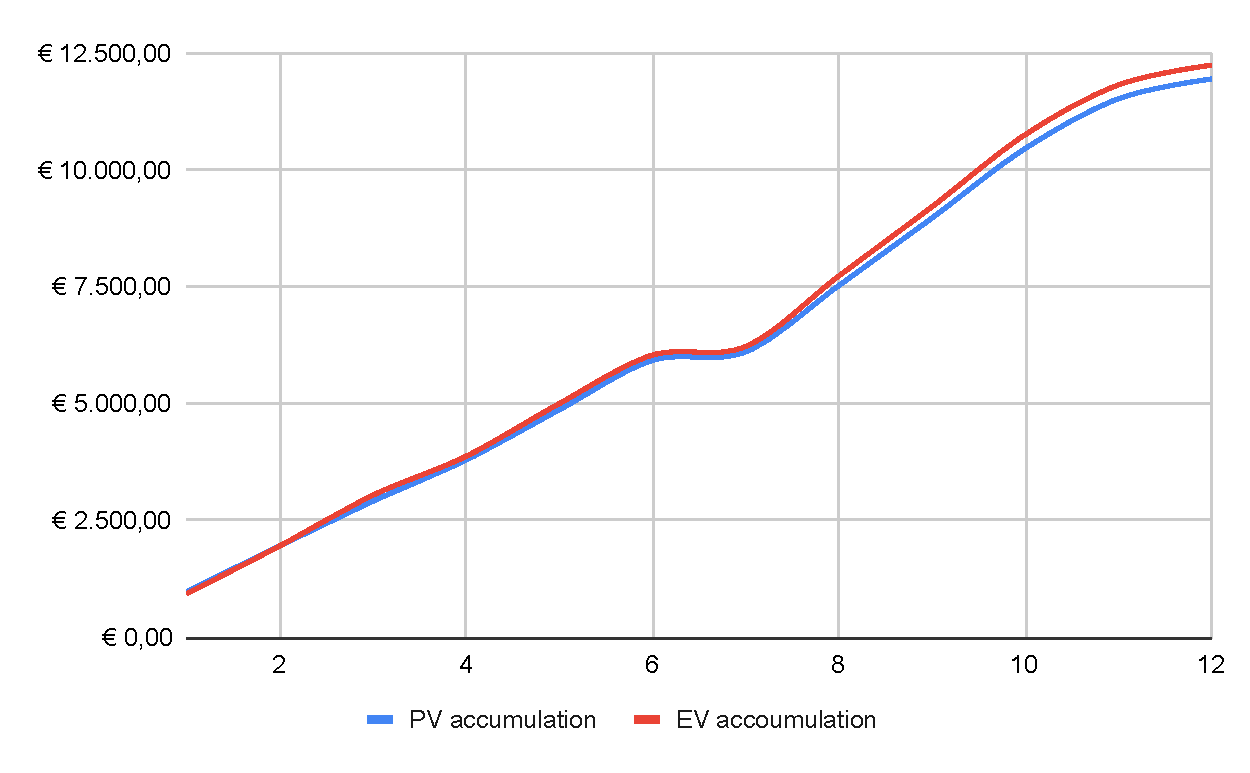
\includegraphics[width=1\textwidth]{charts/pv-ev.pdf}
    \caption{Comparazione \textit{Planned Value - Earned Value}}
    \label{fig:pv-ev}
\end{figure}

\subsection{Confronto MPC-AC e MPC-ETC}
\begin{table}[H]
    \centering
	\begin{tabular}{|c|l|l|l|p{2.6cm}|}
		\hline
		\textbf{Sprint} & \textbf{Actual Cost} & \textbf{Accumulo AC} & \textbf{Estimate to Complete} & \textbf{Estimate at Completion} \\
		\hline
		1 & €945,00 & €945,00 & €11.994,61 & €12.939,61 \\ 
		\hline
        2 & €980,00 & €1.925,00 & €10.375,87 & €12.300,87 \\
        \hline
        3 & €1.105,00 & €3.030,00 & €10.064,31 & €13.094,31 \\
        \hline
        4 & €780,00 & €3.810,00 & €8.239,99 & €12.049,99 \\
        \hline
        5 & €1.120,00 & €4.930,00 & €7.859,31 & €12.789,31 \\
        \hline
        6 & €1.040,00 & €5.970,00 & €6.925,73 & €12.895,73 \\
        \hline
        7 & €185,00 & €6.155,00 & €6.705,00 & €12.860,00 \\
        \hline
        8 & €1.495,00 & €7.650,00 & €5.125,90 & €12.775,90 \\
        \hline
        9 & €1.505,00 & €9.155,00 & €3.904,13 & €13.059,13 \\
        \hline
        10 & €1.535,00 & €10.690,00 & €2.128,25 & €12.818,25 \\
        \hline
        11 & €1.085,00 & €11.775,00 & €1.326,50 & €13.101,50 \\
        \hline
        12 & €275,00 & €12.050,00 & €810,00 & €12.860,00 \\
        \hline
	\end{tabular}
	\caption{MPC-AC, MPC-ETC e MPC-EAC per sprint}
	\label{tab:ac-etc}
\end{table}

\subsubsection{RTB}
L'analisi del grafico in Figura \ref{fig:ac-etc} evidenzia, come atteso, un incremento progressivo dell'\textit{Actual Cost}, fisiologico e coerente con il continuo assorbimento delle risorse economiche durante l'avanzamento del progetto.
Relativamente alle metriche previsionali \textit{Estimate to Complete} ed \textit{Estimate at Completion}, osserviamo un trend decrescente fino al secondo sprint. Tale dinamica rappresenta un indicatore di elevata efficienza iniziale, avendo posizionato la stima del costo a finire (EAC) significativamente al di sotto del budget stanziato.
Tra il secondo e il terzo sprint, tuttavia, rileviamo una flessione nelle performance di progetto: all'incremento dei costi sostenuti non corrisponde una proporzionale riduzione del lavoro residuo stimato (ETC). Conseguentemente, l'EAC subisce un innalzamento, approssimandosi al limite critico definito dal BAC. Questa deviazione è imputabile principalmente alla fase di revisione dell'\textit{Analisi dei Requisiti}, un'attività che ha richiesto un notevole impiego di risorse in termini di \textit{effort} senza tuttavia generare un proporzionale incremento del valore maturato (\textit{Earned Value}). A tale criticità si è sommata un'iniziale inesperienza nella pianificazione operativa e nel coordinamento delle attività del team, con inevitabili ricadute negative sull'efficienza economica complessiva dello sprint.
A partire dal terzo sprint si registra, in controtendenza, un marcato recupero dell'efficienza operativa, con una riduzione dell'ETC. Ciò determina una conseguente e significativa riduzione della stima del costo totale a finire. Pur riscontrando un lieve incremento dell'EAC in corrispondenza del quinto sprint, la proiezione di chiusura si stabilizza circa al limite imposto dal BAC. Valutazione:
\begin{itemize}
    \item \textbf{Valore accettabile:} AC$>0$€, vincolo \textit{rispettato}.
    \item \textbf{Valore ottimo:} AC$\leq$EAC, vincolo \textit{rispettato}.
    \item \textbf{Valore accettabile:} ETC$\geq 0$, vincolo \textit{rispettato}.
    \item \textbf{Valore ottimo:} ETC$\geq 0$, vincolo \textit{rispettato}.
\end{itemize}

\subsubsection{PB}
Analizzando l'intervallo compreso tra lo Sprint 8 e lo Sprint 12 visibile in FIgura \ref{fig:ac-etc}, si osserva il progressivo esaurimento delle attività di progetto, evidenziato dalla curva dell'\textit{Estimate to Complete (ETC)} che decresce verso lo zero. Di conseguenza, l'\textit{Actual Cost (AC)} cumulato rallenta la sua ascesa fino a stabilizzarsi, consolidando una proiezione del costo finale (\textit{Estimate at Completion}) lineare e priva di scostamenti critici. 
Mantenendosi al di sotto del \textit{Budget at Completion (BAC)}, l'EAC certifica la chiusura del progetto in economia, nel pieno rispetto dell'assunzione nella dichiarazione degli impegni.
\begin{itemize}
    \item \textbf{Valore accettabile:} AC$>0$€, vincolo \textit{rispettato}.
    \item \textbf{Valore ottimo:} AC$\leq$EAC, vincolo \textit{rispettato}.
    \item \textbf{Valore accettabile:} ETC$\geq 0$, vincolo \textit{rispettato}.
    \item \textbf{Valore ottimo:} ETC$\geq 0$, vincolo \textit{rispettato}.
\end{itemize}

\begin{figure}[H]
    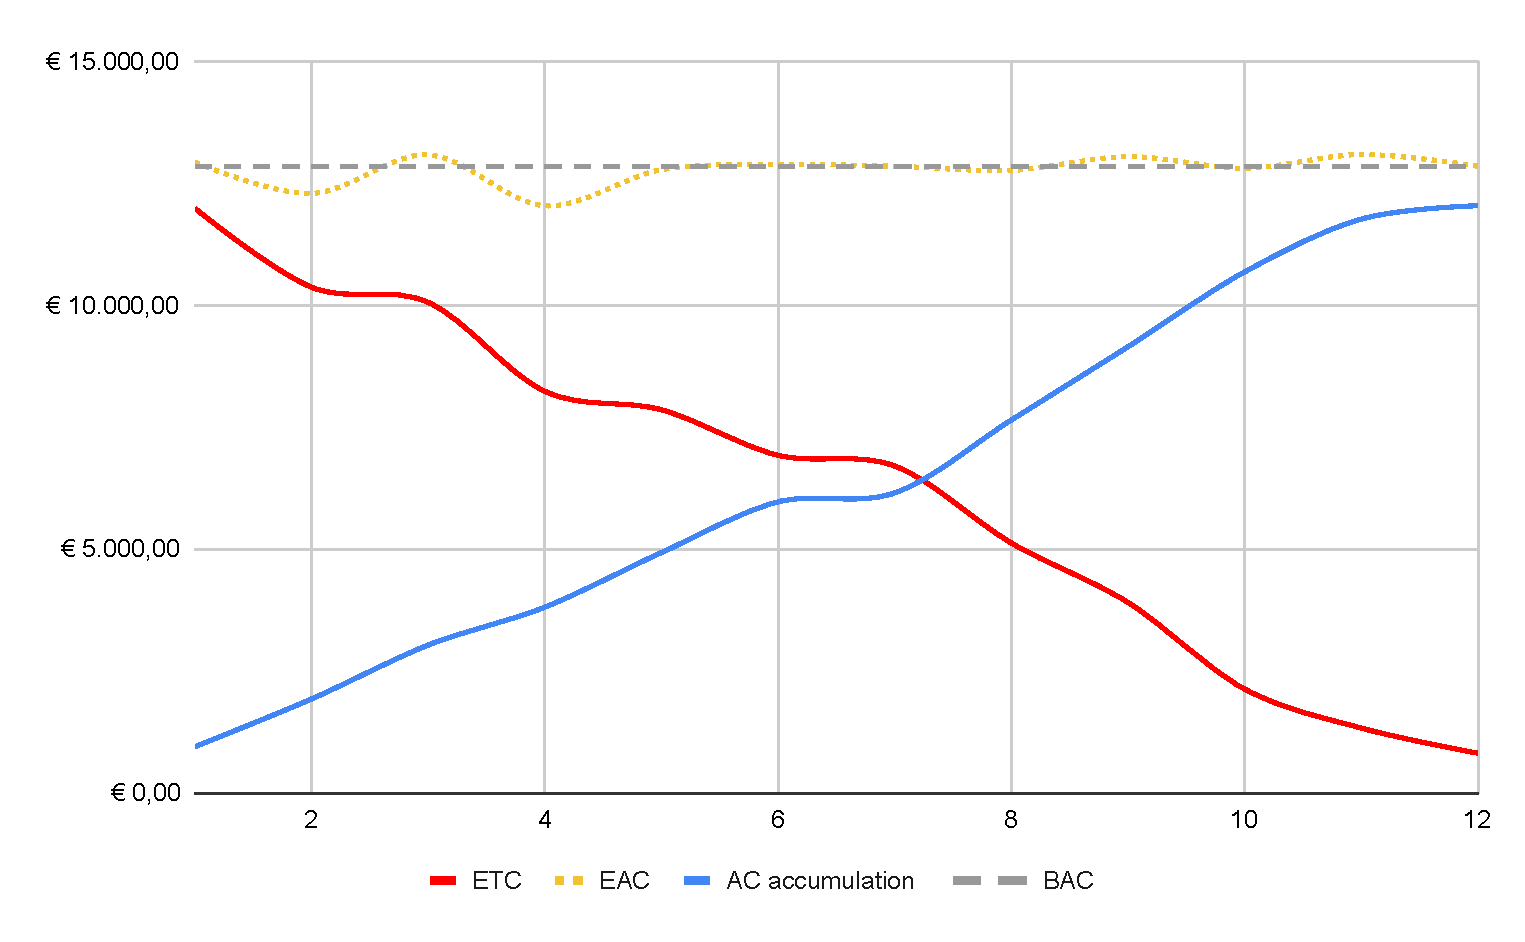
\includegraphics[width=1\textwidth]{charts/ac-etc.pdf}
    \caption{Comparazione \textit{Actual Cost - Estimate to Complete - Estimated at Completion}}
    \label{fig:ac-etc}
\end{figure}

\subsection{Confronto MPC-CV e MPC-SV}
\begin{table}[H]
    \centering
	\begin{tabular}{|c|l|l|p{3cm}|}
		\hline
		\textbf{Sprint} & \textbf{Cost Variance (€)} & \textbf{Schedule Variance (€)} & \textbf{Giudizio} \\
		\hline
		1 & -5,81 & -45,81 & In ritardo e lievemente sopra il budget\\ 
		\hline
        2 & +44,55 & +44,55 & In anticipo e sotto il budget \\
        \hline
        3 & -19,77 & +130,23 & In anticipo ma sopra il budget \\
        \hline
        4 & +52,43 & -47,57 & In ritardo ma sotto il budget \\
        \hline
        5 & +6,19 & +51,19 & In anticipo e lievemente sotto il budget \\
        \hline
        6 & -2,88 & -17,88 & In ritardo e lievemente sopra il budget \\
        \hline
        7 & 0,00 & 0,00 & In regola \\
        \hline
        8 & +9,84 & +89,84 & In anticipo e sotto il budget \\
        \hline
        9 & -22,95 & +37,05 & In anticipo ma sopra il budget \\
        \hline
        10 & +5,00 & +55,00 & In anticipo e sotto il budget \\
        \hline
        11 & -20,00 & 0,00 & In orario ma sopra il budget \\
        \hline
        12 & 0,00 & 0,00 & In regola \\
        \hline
	\end{tabular}
	\caption{MPC-CV e MPC-SV per sprint}
	\label{tab:cv-sv}
\end{table}

\subsubsection{RTB}
Dall'analisi del grafico in Figura \ref{fig:cv-sv} possiamo notare un andamento altalenante che, tuttavia, culmina in una convergenza verso l'efficienza ottimale:
\begin{itemize}
    \item \textbf{Sprint 1:} In questo sprint il progetto si avvia con performance al di sotto del livello di ottimalità. Questa dinamica è del tutto coerente con le difficoltà iniziali di calibrazione del team.
    \item \textbf{Sprint 2:} In questo sprint il team recupera il ritardo iniziale con un ottimo slancio portandosi in anticipo sulle consegne. Questo slancio, però, comporta un impiego di risorse economiche superiore al previsto, che porta ad uno scenario di anticipo temporale a fronte di un sovraccosto.
    \item \textbf{Sprint 3:} La tendenza all'accelerazione vista nello scorso sprint si consolida generando il picco massimo di vantaggio sulla schedulazione. Questo ritmo veloce produce un ulteriore, seppur contenuto, sforamento del budget.
    \item \textbf{Sprint 4:} In questo sprint il team registra una flessione dal punto di vista temporale, accumulando nuovamente ritardo rispetto al piano ideale. Di contro si rileva un eccellente recupero dell'efficienza economica.
    \item \textbf{Sprint 5:} In questa iterazione entrambe le metriche di varianza risultano positive consolidando un solido anticipo sulla tabella di marcia mantenendo allo stesso tempo una, seppur minima, efficienza finanziaria.
    \item \textbf{Sprint 6:} In questo sprint il progetto registra un leggero calo delle prestazioni dovuto principalmente alla sessione d'esami. Questo ha portato ad un ritardo contenuto e ad un leggero sforamento di budget.
    \item \textbf{Sprint 7:} In quest'ultima iterazione analizzata notiamo \textit{Schedule Variance} e \textit{Cost Variance} pari a zero. Questo è dovuto dal fatto che questo sprint rappresentava la prima fase di revisione RTB, quindi il carico di lavoro è stato poco e facile da portare a termine. 
\end{itemize}
Valutazione: 
\begin{itemize}
    \item \textbf{Valore accettabile CV:} $CV>0$, vincolo \textit{violato} in tre sprint su cinque con scostamenti lievi.
    \item \textbf{Valore accettabile SV:} $SV\geq 0$, vincolo \textit{violato} in tre sprint su cinque con slittamenti consistenti.
\end{itemize}

\subsubsection{PB}
Di seguito la valutazione, sprint per sprint, della fase visibile in Figura \ref{fig:cv-sv}:
\begin{itemize}
\item \textbf{Sprint 8:} Con la ripresa delle attività di sviluppo a pieno regime dopo la revisione, il team registra una performance solida. Le metriche di varianza si assestano, garantendo il rispetto delle tempistiche e un buon controllo sul budget.
\item \textbf{Sprint 9:} In questa fase, si osserva un progressivo consolidamento dell'efficienza operativa seppur con un leggero sforamento economico. Questo sforamento è dovuto al rallentamento fisiologico che il progetto ha subito il team durante i mesi scarichi da impegni universitari.
\item \textbf{Sprint 10:} L'iterazione conferma il trend virtuoso intrapreso. L'avvicinamento alle fasi finali di \textit{delivery} procede speditamente, con le curve di \textit{Cost Variance} e \textit{Schedule Variance} che testimoniano un'ottima gestione delle risorse residue.
\item \textbf{Sprint 11:} Avviandosi verso la conclusione delle attività principali, la \textit{Schedule Variance} inizia la sua fisiologica convergenza verso lo zero, a indicare che il lavoro in sospeso si sta esaurendo esattamente secondo le scadenze del piano originario. Si nota però un leggero sforamento economico. 
\item \textbf{Sprint 12:} Nell'ultimo sprint analizzato, la \textit{Schedule Variance} si azzera definitivamente, certificando il completamento del lavoro pianificato senza alcun ritardo finale. La \textit{Cost Variance} si attesta su un valore di chiusura positivo, mostrando il completamento del progetto in efficienza economica.
\end{itemize}
Valutazione: 
\begin{itemize}
    \item \textbf{Valore accettabile CV:} $CV>0$, vincolo \textit{violato} in due sprint su cinque con scostamenti lievi.
    \item \textbf{Valore accettabile SV:} $SV\geq 0$, vincolo \textit{rispettato}.
    \item \textbf{Valore ottimo SV:} $SV > 0$, vincolo \textit{violato} in due sprint su cinque. 
\end{itemize}

\begin{figure}[H]
    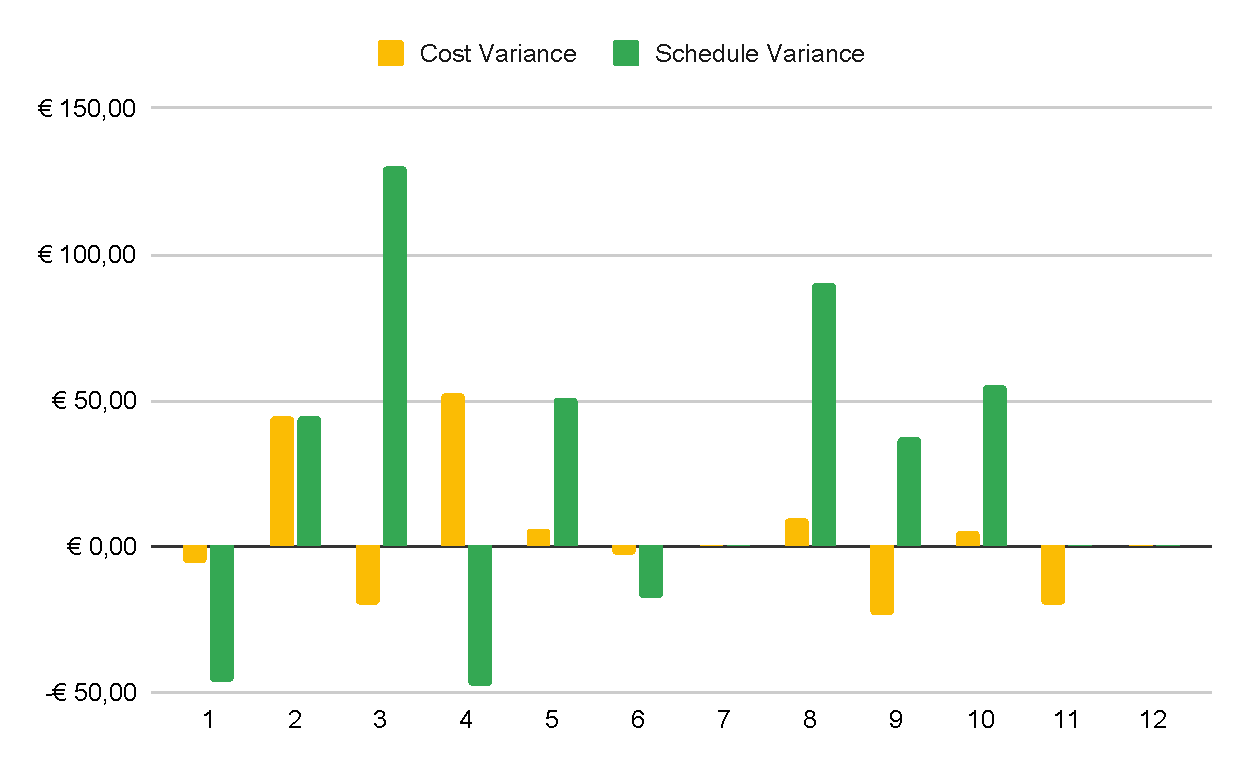
\includegraphics[width=1\textwidth]{charts/cv-sv.pdf}
    \caption{Comparazione \textit{Cost Variance - Schedule Variance}}
    \label{fig:cv-sv}
\end{figure}

\subsection{Confronto MPC-EAC e MPC-BAC}
\begin{table}[H]
    \centering
	\begin{tabular}{|c|l|l|p{3cm}|}
		\hline
		\textbf{Sprint} & \textbf{Estimate At Completion} & \textbf{Budget At Completion} & \textbf{Stato} \\
		\hline
		1 & €12.939,61 & €12.860,00 & EAC$>$BAC \\ 
		\hline
        2 & €12.300,87 & €12.860,00 & EAC$<$BAC \\
        \hline
        3 & €13.094,31 & €12.860,00 & EAC$>$BAC \\
        \hline
        4 & €12.049,99 & €12.860,00& EAC$<$BAC \\
        \hline
        5 & €12.789,31 & €12.860,00 & EAC$<$BAC \\
        \hline
        6 & €12.895,73 & €12.860,00 & EAC$>$BAC \\
        \hline
        7 & €12.860,00 & €12.860,00 & EAC$=$BAC \\
        \hline
        8 & €12.775,90 & €12.860,00 & EAC$<$BAC \\
        \hline
        9 & €13.059,13 & €12.860,00 & EAC$>$BAC \\
        \hline
        10 & €12.818,25 & €12.860,00 & EAC$<$BAC \\
        \hline
        11 & €13.101,50 & €12.860,00 & EAC$>$BAC \\
        \hline
        12 & €12.860,00 & €12.860,00 & EAC$=$BAC \\
        \hline
	\end{tabular}
	\caption{MPC-EAC e BAC per sprint}
	\label{tab:eac-bac}
\end{table}

\subsubsection{RTB}
Dall'aggiudicazione del capitolato fino alla revisione della RTB, l'\textit{Estimate At Completion} oscilla attorno al \textit{Budget At Completion}. L'EAC supera il BAC solo in tre occasioni:
\begin{itemize}
    \item \textbf{Sprint 1:} come detto anche nelle altre sezioni, il primo sprint ha sofferto dell'inesperienza del gruppo nell'organizzare le task, dimensionarle e portarle a compimento. Questo ha provocato un leggero sforamento di budget.
    \item \textbf{Sprint 3:} in questo sprint il gruppo si è dovuto confrontare con la revisione dell'\textit{Analisi dei Requisiti}, che ha portato ad un rallentamento del progetto e ad un conseguente minore valore aggiunto.
    \item \textbf{Sprint 6:} in questo sprint il gruppo ha dovuto affrontare la revisione interna dei documenti e del PoC precedente alla prima fase di revisione RTB. Questo ha portato ad un carico di lavoro importante con conseguente sforamento di budget e leggero ritardo in quanto non si è prodotto un effettivo valore aggiunto.
\end{itemize} 
Valutazione:
\begin{itemize}
    \item \textbf{Valore accettabile:} EAC$\leq 110\%$ budget, vincolo \textit{rispettato}.
    \item \textbf{Valore ottimale:} EAC$\leq$ budget, vincolo \textit{violato} in tre sprint su cinque.
\end{itemize}

\subsubsection{PB}
Analizzando il grafico in Figura \ref{fig:eac-bac} relativo all'andamento dell'\textit{Estimate at Completion (EAC)} in rapporto al \textit{Budget at Completion (BAC)}, si osserva un'oscillazione della spesa totale prevista durante le iterazioni conclusive del progetto. 
Nello sprint 9 e 11, infatti, l'EAC si posiziona di poco sopra al budget concordato. Questo è frutto delle naturali oscillazioni di prestazione lavorativa del gruppo durante gli sprint finali. 
Nonostante ciò, lo sprint 12 chiude in linea con il BAC, assicurando che il progetto si concluda in economia senza alcun rischio di sforamento del budget originario.
Valutazione:
\begin{itemize}
    \item \textbf{Valore accettabile:} EAC$\leq 110\%$ budget, vincolo \textit{rispettato}.
    \item \textbf{Valore ottimale:} EAC$\leq$ budget, vincolo \textit{violato} in tre sprint su cinque.
\end{itemize}

\begin{figure}[H]
    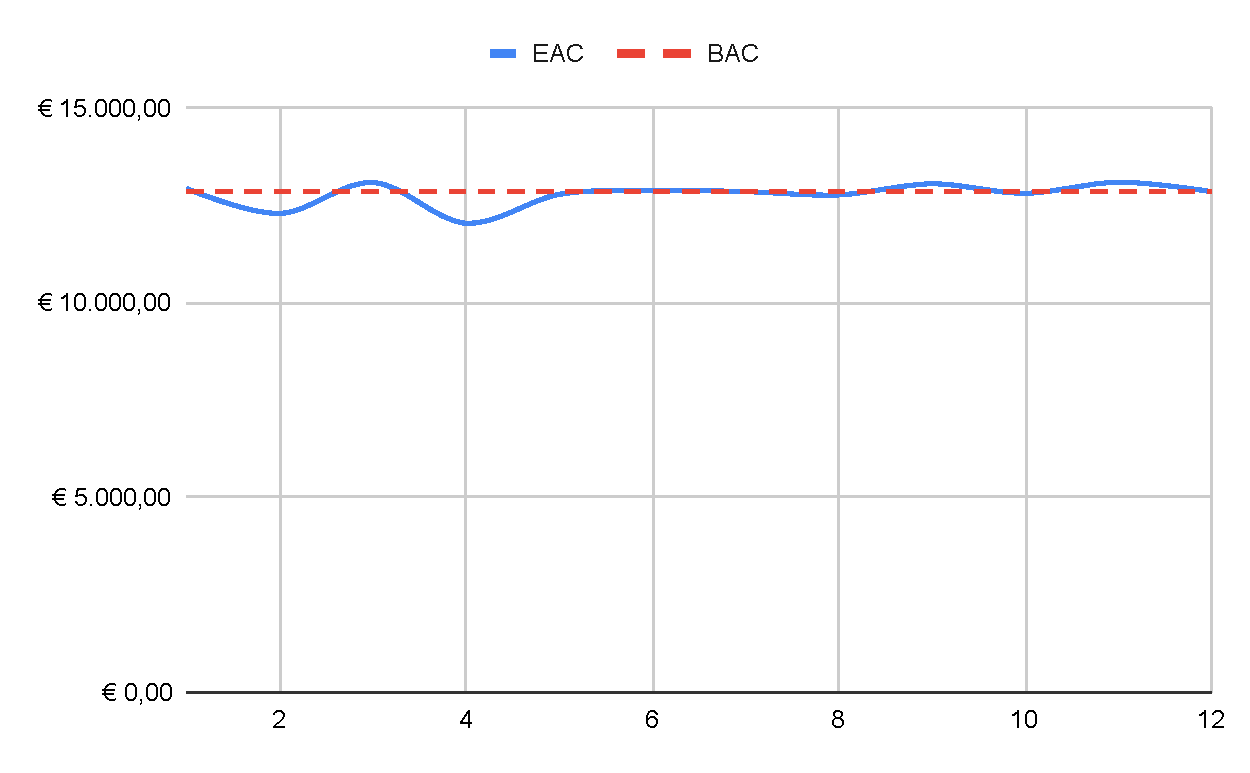
\includegraphics[width=1\textwidth]{charts/eac-bac.pdf}
    \caption{Comparazione \textit{Estimate At Completion - Budget At Completion}}
    \label{fig:eac-bac}
\end{figure}

\subsection{Valutazione MPC-TCR}
\begin{table}[H]
    \centering
	\begin{tabular}{|c|l|l|l|p{3cm}|}
		\hline
		\textbf{Sprint} & \textbf{Task completate} & \textbf{Task in ritardo} & \textbf{TCR (\%)} & \textbf{Giudizio} \\
		\hline
		1 & 13 & 3 & $76,9\%$ & Critico\\ 
		\hline
        2 & 11 & 0 & $100,0\%$ & Ottimo \\
        \hline
        3 & 13 & 0 & $100,0\%$ & Ottimo \\
        \hline
        4 & 13 & 1 & $92,3\%$ & Accettabile \\
        \hline
        5 & 49 & 0 & $100,0\%$ & Ottimo  \\
        \hline
        6 & 25 & 0 & $100,0\%$ & Ottimo \\
        \hline
        7 & 5 & 0 & $100,0\%$ & Ottimo \\
        \hline
        8 & 7 & 0 & $100,0\%$ & Ottimo \\
        \hline
        9 & 14 & 0 & $100,0\%$ & Ottimo \\
        \hline
        10 & 54 & 0 & $100,0\%$ & Ottimo \\
        \hline
        11 & 31 & 0 & $100,0\%$ & Ottimo \\
        \hline
        12 & 5 & 0 & $100,0\%$ & Ottimo \\
        \hline
	\end{tabular}
	\caption{Task Completion Rate per sprint}
	\label{tab:tcr}
\end{table}

\subsubsection{RTB}
Il \textit{Task Completion Rate} risulta ottimo in tre sprint su cinque. Notiamo subottimalità critica nello sprint 1 ($76,9\%$) e una subottimalità lieve nello sprint 4 ($92,3\%$). Valutazione:
\begin{itemize}
    \item \textbf{Valore accettabile:} $TCR \geq 85\%$, vincolo \textit{violato} nello sprint 1.
\end{itemize}

\subsubsection{PB}
Come notiamo dal grafico in Figura \ref{fig:tcr}, il \textit{Task Completion Rate} risulta ottimo in tutti gli sprint finali. Questo è dovuto all'esperienza che il gruppo ha acquisito durante il progetto che ha permesso di gestire carichi di lavoro importanti (e.g. 54 task nello sprint 10) senza particolari problemi di scheduling. Valutazione:
\begin{itemize}
    \item \textbf{Valore accettabile:} $TCR \geq 85\%$, vincolo \textit{rispettato}.
    \item \textbf{Valore ottimale:} $TCR = 100\%$, vincolo \textit{rispettato}.
\end{itemize}
\begin{figure}[H]
    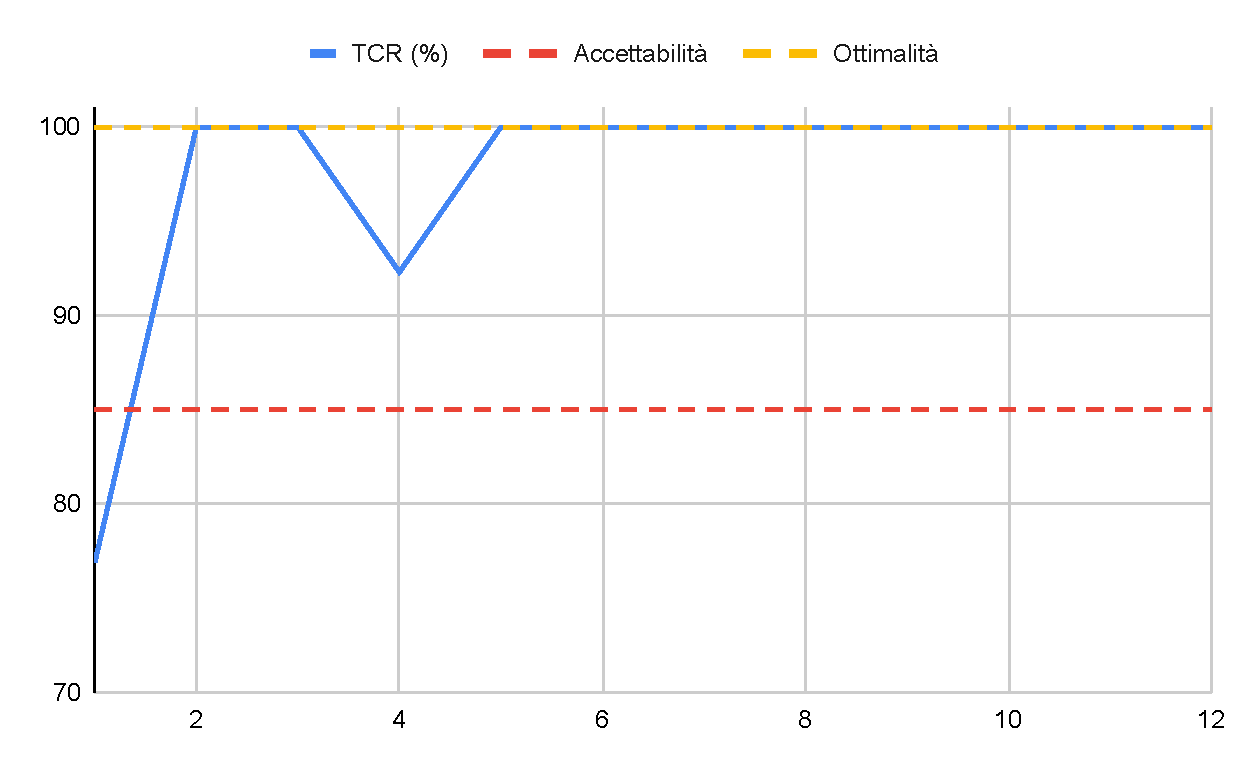
\includegraphics[width=1\textwidth]{charts/tcr.pdf}
    \caption{Valutazione \textit{Task Completion Rate}}
    \label{fig:tcr}
\end{figure}

\subsection{Valutazione MPC-TS}
\begin{table}[H]
    \centering
	\begin{tabular}{|c|l|l|l|p{3cm}|}
		\hline
		\textbf{Sprint} & \textbf{Task completate} & \textbf{Task in ritardo} & \textbf{TS (\%)} & \textbf{Giudizio} \\
		\hline
		1 & 13 & 3 & $23,1\%$ & Critico\\ 
		\hline
        2 & 11 & 0 & $0,0\%$ & Ottimo \\
        \hline
        3 & 13 & 0 & $0,0\%$ & Ottimo \\
        \hline
        4 & 13 & 1 & $7,7\%$ & Accettabile \\
        \hline
        5 & 49 & 0 & $0,0\%$ & Ottimo  \\
        \hline
        6 & 25 & 0 & $0,0\%$ & Ottimo \\
        \hline
        7 & 5 & 0 & $0,0\%$ & Ottimo \\
        \hline
        8 & 7 & 0 & $0,0\%$ & Ottimo \\
        \hline
        9 & 14 & 0 & $0,0\%$ & Ottimo \\
        \hline
        10 & 54 & 0 & $0,0\%$ & Ottimo \\
        \hline
        11 & 31 & 0 & $0,0\%$ & Ottimo \\
        \hline
        12 & 5 & 0 & $0,0\%$ & Ottimo \\
        \hline
	\end{tabular}
	\caption{Task Slippage per sprint}
	\label{tab:ts}
\end{table}

\subsubsection{RTB}
Il \textit{Task Slippage} risulta ottimo in tre sprint su cinque. Notiamo subottimalità critica nello sprint 1 ($23,1\%$) e una subottimalità lieve nello sprint 4 ($7,7\%$). Valutazione:
\begin{itemize}
    \item \textbf{Valore accettabile:} $TS < 15\%$, vincolo \textit{violato} nello sprint 1.
\end{itemize}

\subsubsection{PB}
Ugualmente a quello che succede per l'\textit{MPC-TCR}, negli sprint relativi alla PB, il \textit{Task Slippage} risulta ottimo in tutti e cinque gli sprint. Questo è dovuto alla maturità organizzativa sviluppata durante il progetto che ha permesso di gestire tutti i flussi di lavoro senza particolari problemi. Valutazione:
\begin{itemize}
    \item \textbf{Valore accettabile:} $TS < 15\%$, vincolo \textit{rispettato}.
    \item  \textbf{Valore ottimale:} $TS = 0\%$, vincolo \textit{rispettato}.
\end{itemize}
\begin{figure}[H]
    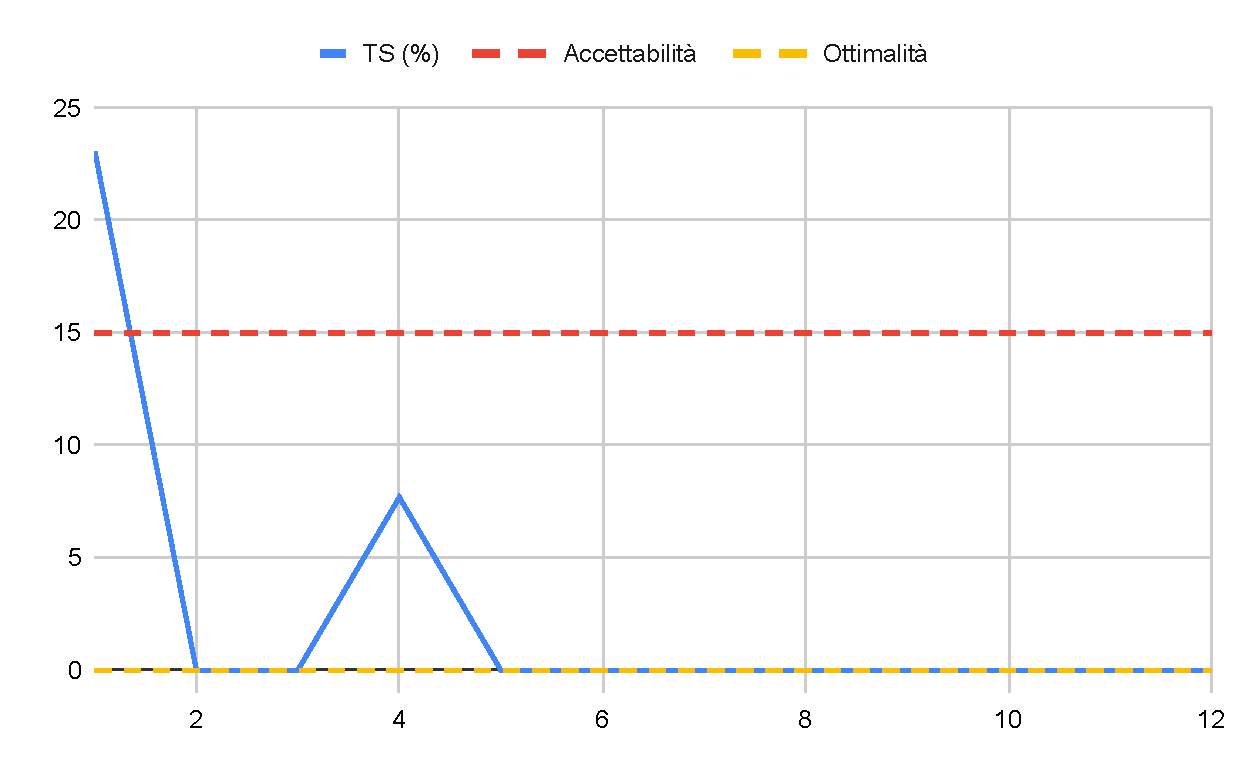
\includegraphics[width=1\textwidth]{charts/ts.pdf}
    \caption{Valutazione \textit{Task Slippage}}
    \label{fig:ts}
\end{figure}

\subsection{Valutazione MPC-MR}
\begin{table}[H]
    \centering
	\begin{tabular}{|c|l|l|l|p{3cm}|}
		\hline
		\textbf{Sprint} & \textbf{Pull request aperte} & \textbf{PR riaperte} & \textbf{MR (\%)} & \textbf{Giudizio} \\
		\hline
		1 & 13 & 1 & $7,7\%$ & Accettabile\\ 
		\hline
        2 & 30 & 2 & $6,7\%$ & Accettabile \\
        \hline
        3 & 21 & 7 & $33,3\%$ & Critico \\
        \hline
        4 & 29 & 7 & $24,1\%$ & Critico \\
        \hline
        5 & 68 & 2 & $2,9\%$ & Ottimo  \\
        \hline
        6 & 30 & 0 & $0,0\%$ & Ottimo \\
        \hline
        7 & 2 & 0 & $0,0\%$ & Ottimo \\
        \hline
        8 & 3 & 0 & $0,0\%$ & Ottimo \\
        \hline
        9 & 9 & 0 & $0,0\%$ & Ottimo \\
        \hline
        10 & 40 & 0 & $0,0\%$ & Ottimo \\
        \hline
        11 & 22 & 0 & $0,0\%$ & Ottimo \\
        \hline
        12 & 4 & 0 & $0,0\%$ & Ottimo \\
        \hline
	\end{tabular}
	\caption{Merge Rework per sprint}
	\label{tab:mr}
\end{table}

\subsubsection{RTB}
Dal grafico in Figura \ref{fig:mr} possiamo notare come la valutazione di \textit{Merge Rework}, ovvero la percentuale di Pull Request approvate nelle quali viene sovrascritto del lavoro già svolto, varia a seconda della fase del progetto. Nei primi due sprint troviamo dei valori simili ($7\%$ circa) che riteniamo accettabili. Questi valori sono dati dal fatto che tutti i membri del gruppo non avevano avuto ancora esperienza di co-working con lo strumento GitHub, né con un progetto con un gruppo così numeroso. Questo ha portato a iniziali incomprensioni sul lavoro da svolgere e, di conseguenza, a riscritture di parti di documenti. Nel terzo e quarto sprint abbiamo valori critici, dovuti principalmente all'\textit{Analisi dei Requisiti} (primo grande documento condiviso da più redattori) e dalla sua riscrittura, dovuta a revisioni a seguito di numerosi difetti di modellazione riscontrati.
Nello sprint 5 abbiamo avuto un'enorme mole di Pull Request dovute all'inizio del \textit{Proof of Concept} che però sono state minimamente sovrascritte grazie ad una progettazione adeguata. Infine negli ultimi due sprint la percentuale di lavoro sovrascritto è stata pari a zero. Questo è dovuto al carico di lavoro diminuito e ad una consapevolezza aumentata sulle task da svolgere e sugli strumenti da utilizzare. Valutazione:
\begin{itemize}
    \item \textbf{Valore accettabile:} $MR \leq 20\%$, vincolo \textit{violato} in due sprint su cinque.
\end{itemize}

\subsubsection{PB}
Come possiamo notare in Figura \ref{fig:mr}, la percentuale di Pull Request approvate nelle quali viene sovrascritto del lavoro già svolto, a differenza di quanto è avvenuto nella fase RTB, rimane stabile sullo zero durante tutta la fase di PB. Questo risultato, così come quelli raggiunti per \textit{MPC-TCR} e \textit{MPC-TS}, denotano una maturità nella pianificazione delle task e nello svolgere il proprio lavoro, che ci ha portato a non perdere più tempo nel mettere nuovamente mano a ciò che era già stato fatto ma nel proseguire spediti verso la fine.
Valutazione:
\begin{itemize}
    \item \textbf{Valore accettabile:} $MR \leq 20\%$, vincolo \textit{rispettato}.
    \item \textbf{Valore ottimale:} $MR \leq 5\%$, vincolo \textit{rispettato}.
\end{itemize}

\begin{figure}[H]
    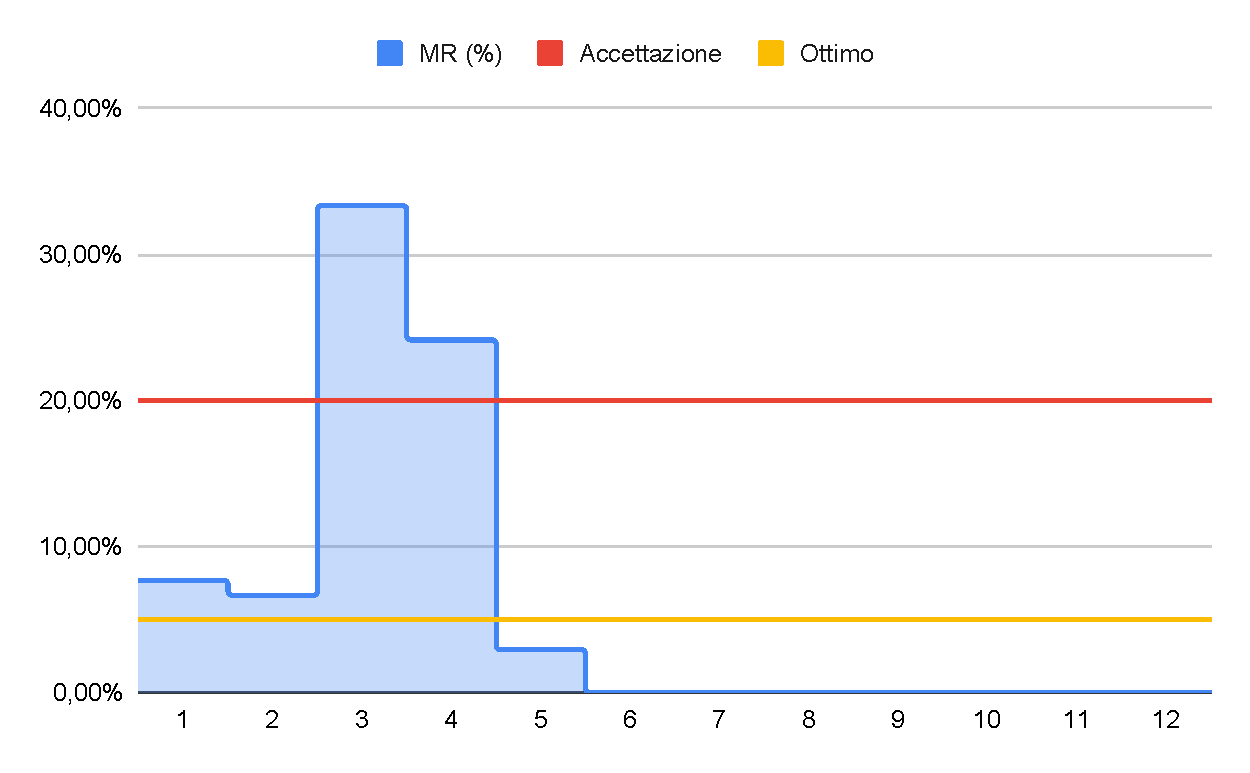
\includegraphics[width=1\textwidth]{charts/mr.pdf}
    \caption{Valutazione \textit{Merge Rework}}
    \label{fig:mr}
\end{figure}

\subsection{Valutazione MPC-IR}
\begin{table}[H]
    \centering
	\begin{tabular}{|c|l|l|l|p{3cm}|}
		\hline
		\textbf{Sprint} & \textbf{Issues aperte} & \textbf{Issues riaperte} & \textbf{IR (\%)} & \textbf{Giudizio} \\
		\hline
		1 & 13 & 0 & $0,0\%$ & Ottimo\\ 
		\hline
        2 & 11 & 1 & $9,1\%$ & Accettabile \\
        \hline
        3 & 13 & 3 & $23,1\%$ & Critico \\
        \hline
        4 & 14 & 0 & $0,0\%$ & Ottimo \\
        \hline
        5 & 49 & 1 & $2,0\%$ & Accettabile  \\
        \hline
        6 & 25 & 0 & $0,0\%$ & Ottimo \\
        \hline
        7 & 5 & 0 & $0,00\%$ & Ottimo\\
        \hline
	\end{tabular}
	\caption{Issue Reopening Rate per sprint}
	\label{tab:ir}
\end{table}
Come è possibile notare in Figura \ref{fig:ir}, l'andamento dell'\textit{Issue Reopening Rate} è altalenante sebbene si mantenga quasi sempre abbondantemente sotto la soglia di accettabilità. L'unico sprint che fa eccezione è il numero 3 che, per motivi già affrontati in questo documento, possiede un valore di MPC-IR critico. Valutazione:
\begin{itemize}
    \item \textbf{Valore accettabile:} $IR \leq 15\%$, vincolo \textit{violato} nello sprint 3.
\end{itemize}

\begin{figure}[H]
    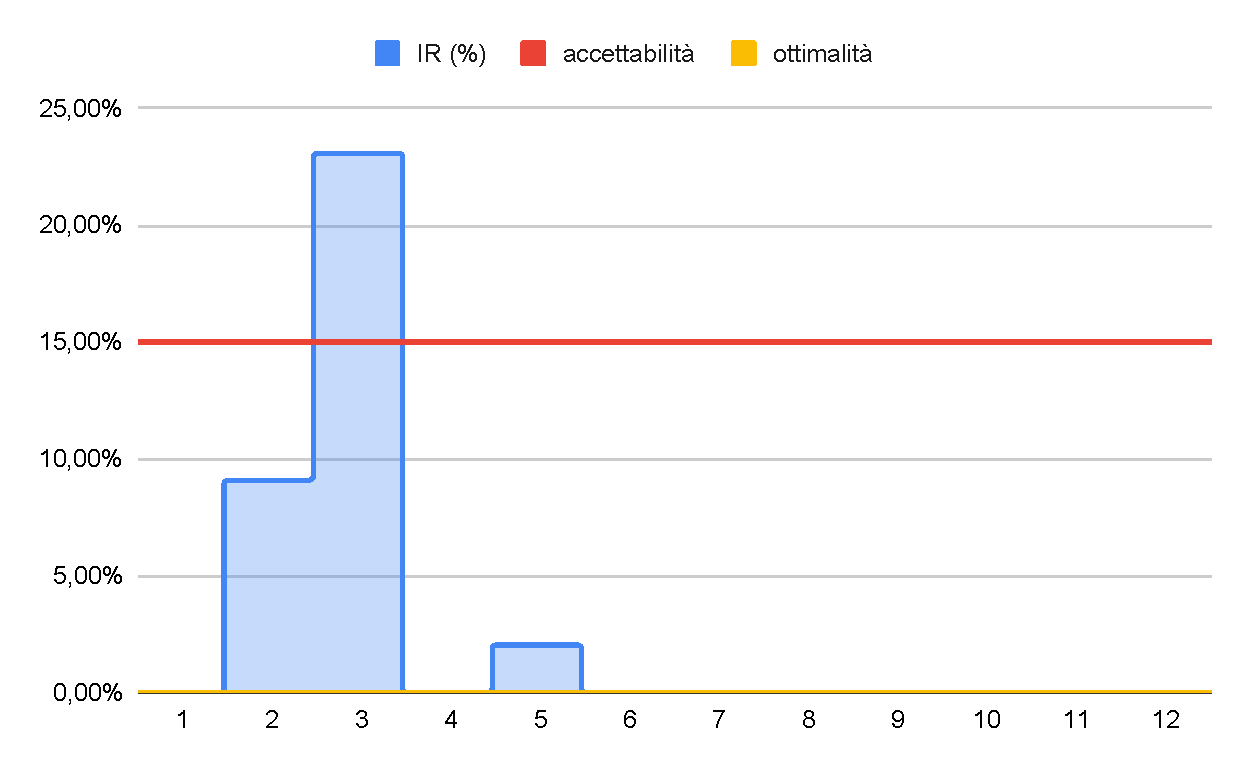
\includegraphics[width=1\textwidth]{charts/ir.pdf}
    \caption{Valutazione \textit{Issue Reopening Rate}}
    \label{fig:ir}
\end{figure}

\subsection{Valutazione MPC-IG}
\begin{table}[H]
    \centering
	\begin{tabular}{|c|l|p{3cm}|}
		\hline
		\textbf{Documento} & \textbf{Indice di Gulpease} & \textbf{Giudizio} \\
		\hline
		AdR & 97 & Ottimo\\ 
		\hline
        Glossario & 75 & Ottimo \\
        \hline
        NdP & 100 & Ottimo \\
        \hline
        PdQ & 86 & Ottimo \\
        \hline
        PdP & 100 & Ottimo  \\
        \hline
	\end{tabular}
	\caption{Indice di Gulpease per documento}
	\label{tab:ig}
\end{table}
Il grafico in Figura \ref{fig:ig} mostra l'indice di Gulpease di ogni documento prodotto nel suo stato finale (versione 1.0.0). Come possiamo notare, tutti i documenti si posizionano sopra la soglia di ottimalità. Questo certifica che i documenti prodotti sono leggibili e comprensibili da qualsiasi individuo in possesso di licenza media. Questa leggibilità elevata è data dalla preferenza di periodi semplici e brevi al posto di quelli complessi e lunghi; in più le parole usate vogliono essere il meno "tecniche" possibili, preferendo quindi una maggiore comprensibilità per i non addetti ai lavori a discapito però di una maggiore lunghezza dei documenti.
Valutazione:
\begin{itemize}
    \item \textbf{Valore accettabile:} $IG \geq 40$, vincolo sempre \textit{rispettato}.
    \item \textbf{Valore ottimo:} $IG \geq 60$, vincolo sempre \textit{rispettato}.
\end{itemize}

\begin{figure}[H]
    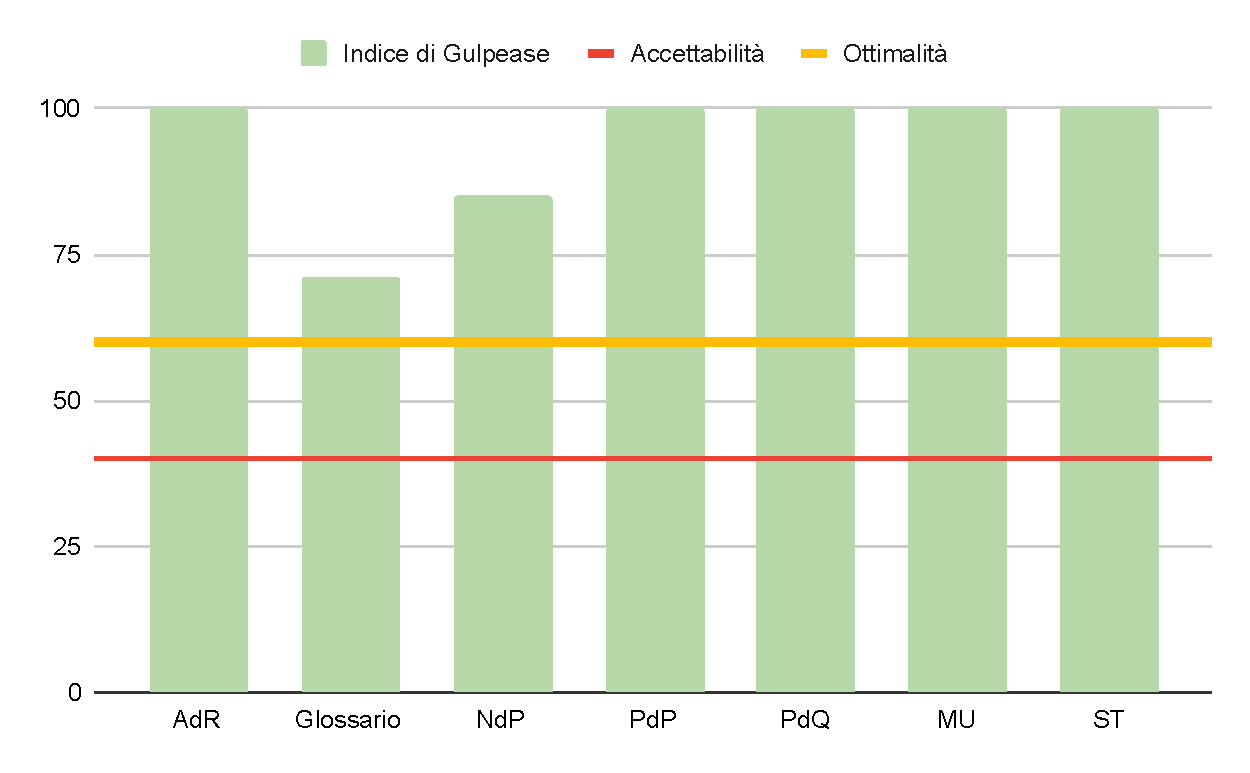
\includegraphics[width=1\textwidth]{charts/ig.pdf}
    \caption{Valutazione \textit{Indice di Gulpease}}
    \label{fig:ig}
\end{figure}


\subsection{Valutazione MPC-CO}
\begin{table}[H]
    \centering
	\begin{tabular}{|c|l|l|l|p{2.2cm}|}
		\hline
		\textbf{Documento} & \textbf{Errori gravi (\%)} & \textbf{Errori non gravi (\%)} & \textbf{CO (\%)} & \textbf{Giudizio} \\
		\hline
		AdR & 0\% & 0,50\% & 99,50\% & Ottimo\\ 
		\hline
        Glossario & 0\% & 1,00\%& 99,00\% & Ottimo \\
        \hline
        NdP & 0\% & 0,30\% & 99,77\% & Ottimo \\
        \hline
        PdQ & 0\% & 0,20\% & 99,80\% & Ottimo \\
        \hline
        PdP & 0\% & 0,28\% & 99,72\% & Ottimo \\
        \hline
	\end{tabular}
	\caption{Percentuale di correttezza ortografica per documento}
	\label{tab:co}
\end{table}
Com'è possibile notare dalla Figura \ref{fig:co}, l'indice di correttezza ortografica è ottimo in tutti i documenti. Questo perché ogni documento in scrittura viene automaticamente analizzato dall'editor di testo che segnala all'utente eventuali inesattezze ortografiche. Valutazione:
\begin{itemize}
    \item \textbf{Valore accettabile:} documenti senza errori gravi, vincolo \textit{rispettato}.
    \item \textbf{Valore ottimo:} $CO \geq 99\%$, vincolo \textit{rispettato}.
\end{itemize}
\begin{figure}[H]
    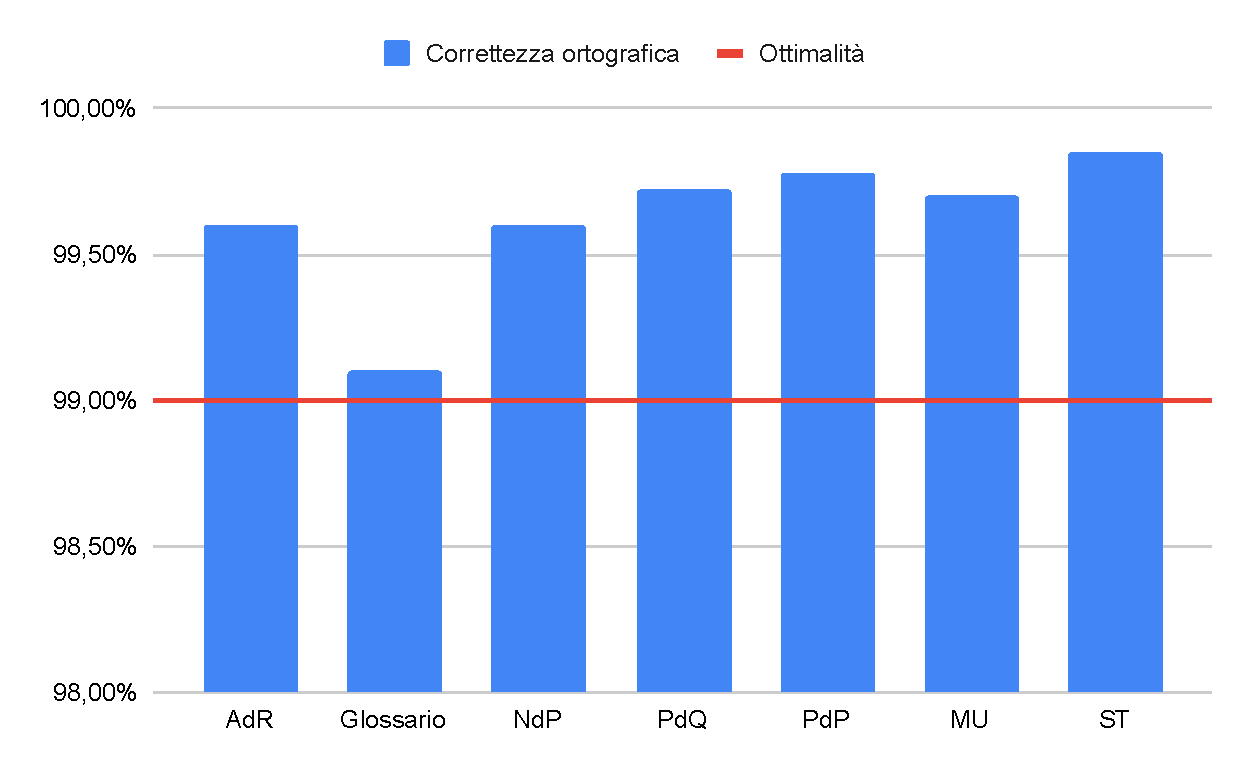
\includegraphics[width=1\textwidth]{charts/co.pdf}
    \caption{Valutazione di \textit{Correttezza Ortografica}}
    \label{fig:co}
\end{figure}

\begin{comment}
\subsection{Valutazione MPC-CD}
\begin{table}[H]
    \centering
	\begin{tabular}{|c|l|p{3cm}|}
		\hline
		\textbf{Documento} & \textbf{Rapporto completezza documentale (\%)} & \textbf{Giudizio} \\
		\hline
		AdR & 100\% & Ottimo\\ 
		\hline
        Glossario & 100\% & Ottimo \\
        \hline
        NdP & 100\% & Ottimo \\
        \hline
        PdQ & 100\% & Ottimo \\
        \hline
        PdP & 100\% & Ottimo  \\
        \hline
	\end{tabular}
	\caption{Percentuale di completezza documentale per documento}
	\label{tab:cd}
\end{table}
L'indice di completezza documentale è ottimo in tutti i documenti, com'è possibile notare in Figura \ref{fig:cd}. Questo perché la struttura di ogni documento in scrittura viene concordata preventivamente nel team e viene verificata ogni qual volta il documento passa alla fase di verifica. Valutazione:
\begin{itemize}
    \item \textbf{Valore accettabile:} $CD \geq 90\%$ delle sezioni previste, vincolo \textit{rispettato}.
    \item \textbf{Valore ottimo:} $CD = 100\%$ delle sezioni previste, vincolo \textit{rispettato}.
\end{itemize}
\begin{figure}[H]
    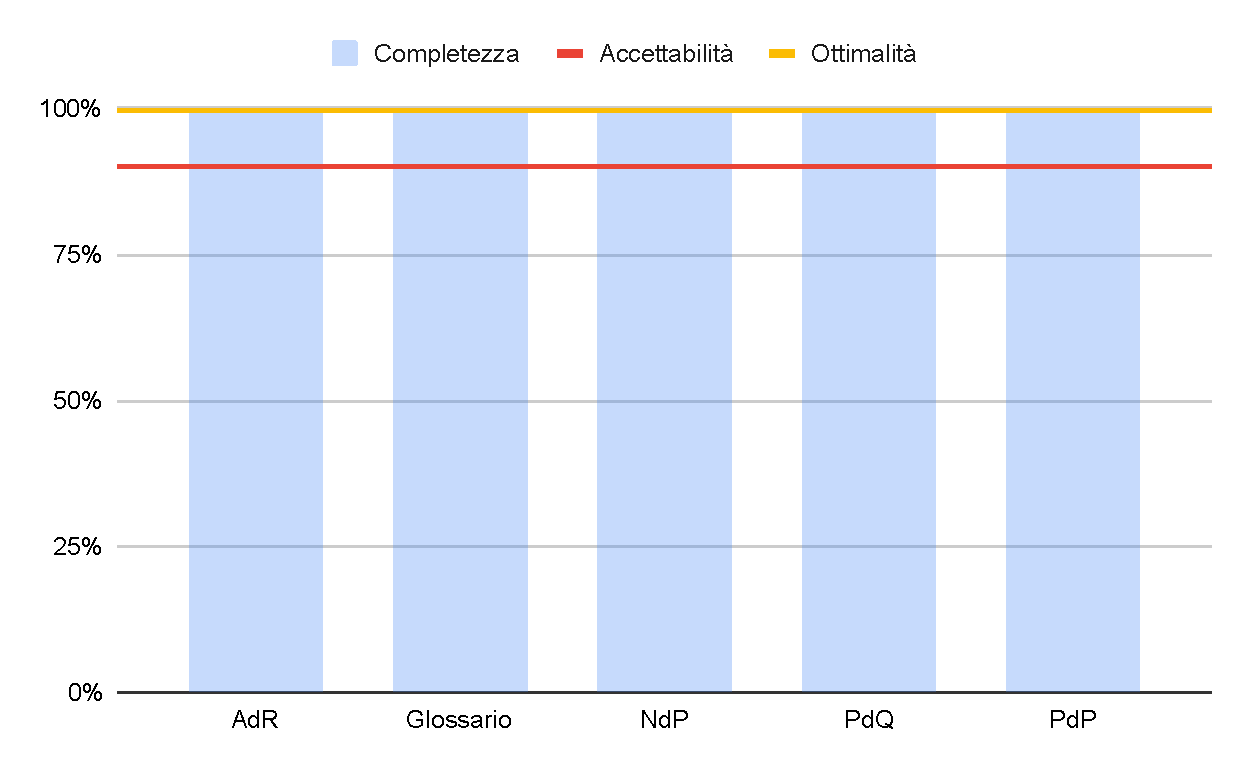
\includegraphics[width=1\textwidth]{charts/cd.pdf}
    \caption{Valutazione \textit{Completezza documentale}}
    \label{fig:cd}
\end{figure}

\subsection{MPC-CR}
\begin{table}[H]
    \centering
	\begin{tabular}{|c|l|p{3cm}|}
		\hline
		\textbf{Documento} & \textbf{Correttezza dei riferimenti (\%)} & \textbf{Giudizio} \\
		\hline
		AdR & 100\% & Ottimo\\ 
		\hline
        Glossario & 100\% & Ottimo \\
        \hline
        NdP & 100\% & Ottimo \\
        \hline
        PdQ & 100\% & Ottimo \\
        \hline
        PdP & 100\% & Ottimo  \\
        \hline
	\end{tabular}
	\caption{Percentuale correttezza dei riferimenti per documento}
	\label{tab:cr}
\end{table}
Dal grafico in Figura \ref{fig:cr} è possibile notare che la percentuale di correttezza dei riferimenti è ottima in ogni documento. Questo perché la correttezza e la coerenza dei riferimenti viene stabilita dal sottogruppo a cui è assegnata la stesura del documento e verificata ogni qual volta il documento passa alla fase di verifica. Valutazione:
\begin{itemize}
    \item \textbf{Valore accettabile:} $CR \geq 95\%$ dei riferimenti validi, vincolo \textit{rispettato}.
    \item \textbf{Valore ottimo:} $CD = 100\%$ dei riferimenti validi, vincolo \textit{rispettato}.
\end{itemize}
\begin{figure}[H]
    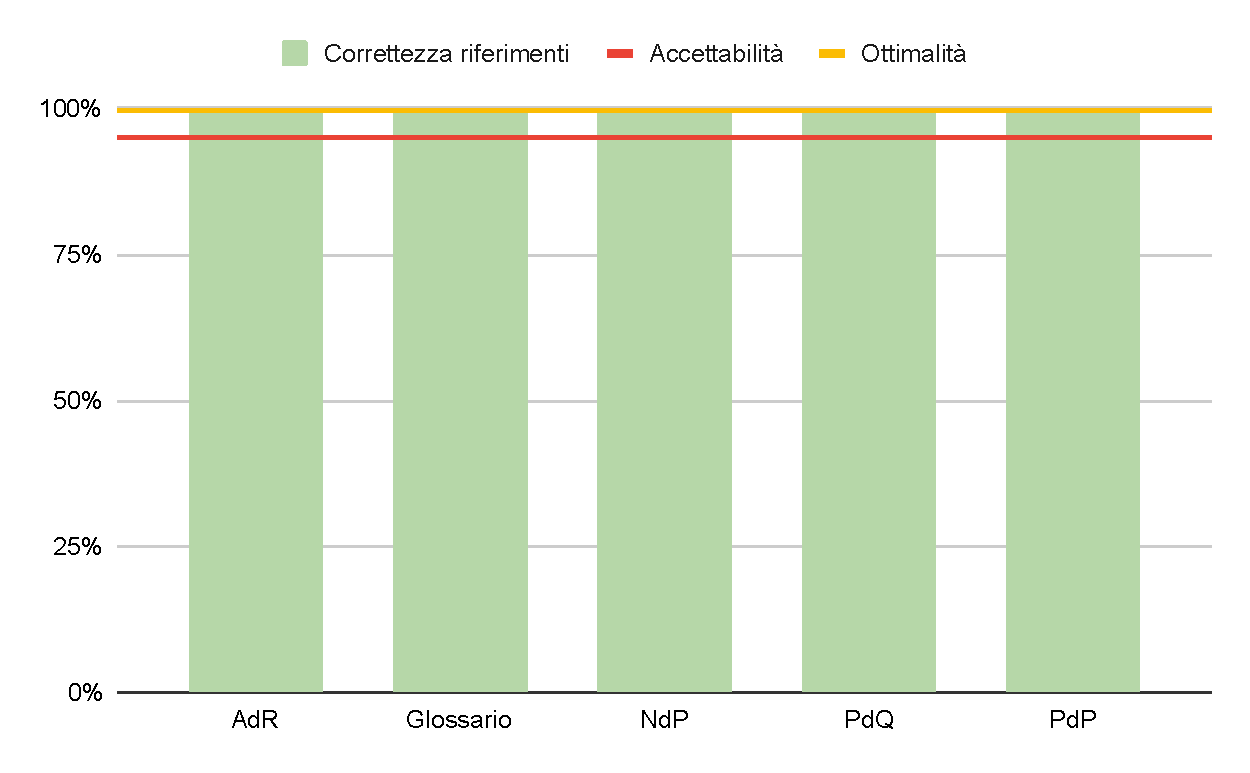
\includegraphics[width=1\textwidth]{charts/cr.pdf}
    \caption{Valutazione \textit{Correttezza dei riferimenti}}
    \label{fig:cr}
\end{figure}

\end{comment}

\subsection{Valutazione MPC-PMS}
\begin{table}[H]
    \centering
	\begin{tabular}{|c|l|p{3cm}|}
		\hline
		\textbf{Sprint} & \textbf{Percentuale Metriche Soddisfatte (\%)} & \textbf{Giudizio} \\
		\hline
		1 & 67\% & Critico\\ 
		\hline
        2 & 100\% & Ottimo \\
        \hline
        3 & 75\% & Critico \\
        \hline
        4 & 83\% & Accettabile \\
        \hline
        5 & 100\% & Ottimo  \\
        \hline
        6 & 82\%& Accettabile \\
        \hline
        7 & 100\% & Ottimo \\
        \hline
	\end{tabular}
	\caption{Percentuale Metriche Soddisfatte per sprint}
	\label{tab:pms}
\end{table}
Analizzando l'andamento della \textit{Percentuale di Metriche Soddisfatte} (MPC-PMS) per la durata degli sprint in Figura \ref{fig:pms}, notiamo un percorso discontinuo ma in miglioramento. A fronte di alcune criticità operative riscontrate negli Sprint 1 e 3 in cui i nostri risultati (67\% e 75\%) sono scesi sotto la soglia di accettabilità dell'80\% per i motivi già citati in questo documento, abbiamo messo in campo un'ottima capacità di reazione. Dopo aver recuperato l'adeguatezza nello Sprint 4 (83\%), nello sprint 5 notiamo un completamento al 100\% delle metriche che ci porta alla piena conformità agli standard qualitativi prefissati. 
Dal calcolo sono state escluse le metriche di correttezza dei documenti, in quanto queste sono calcolate a documento approvato e non a sprint. Il loro coinvolgimento nel calcolo produrrebbe uno sfasamento che non permetterebbe una stima affidabile. Valutazione:
\begin{itemize}
    \item \textbf{Valore accettabile:} $PMS \geq 80\%$, vincolo \textit{non rispettato} nello sprint 1 e 3.
\end{itemize}
\begin{figure}[H]
    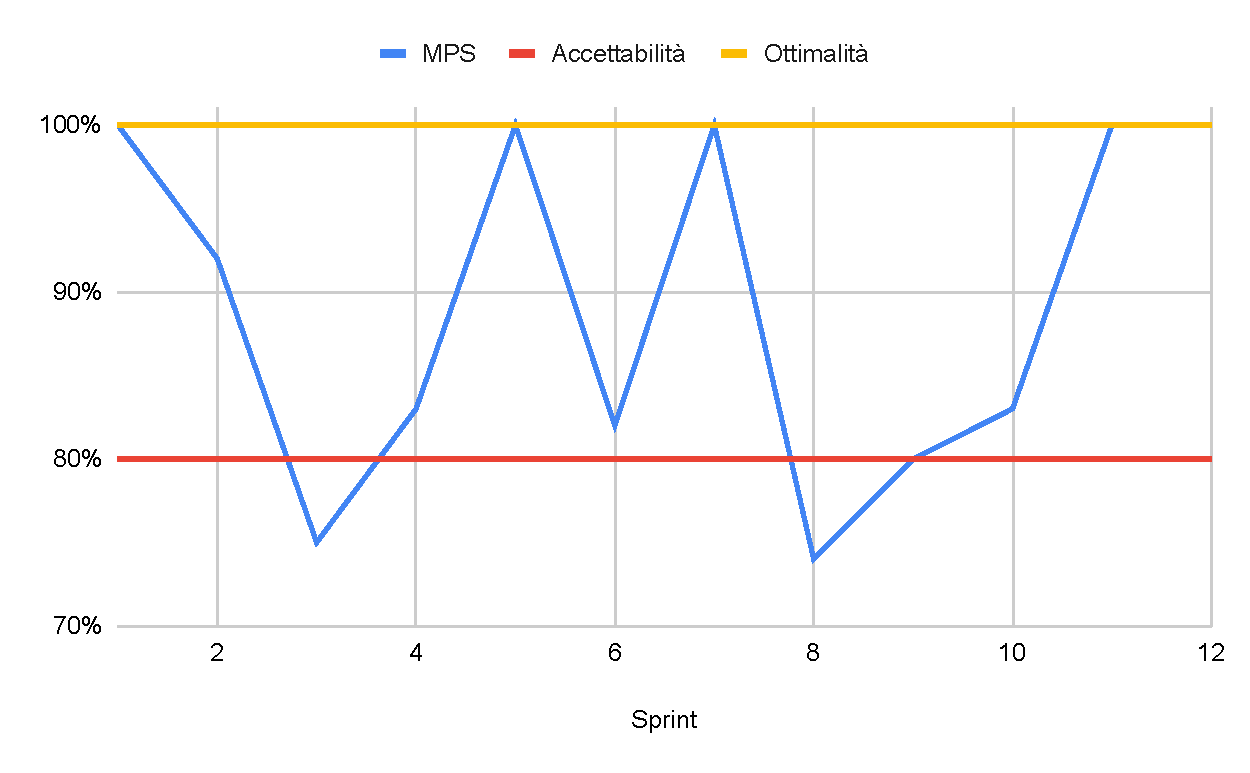
\includegraphics[width=1\textwidth]{charts/pms.pdf}
    \caption{Valutazione \textit{Percentuale di Metriche Soddisfatte}}
    \label{fig:pms}
\end{figure}


\subsection{Valutazione della copertura dei requisiti}
\begin{table}[H]
    \centering
    \small
    \setlength{\tabcolsep}{4pt}
	\begin{tabular}{|c|>{\centering\arraybackslash}p{1.7cm}|>{\centering\arraybackslash}p{1.9cm}|>{\centering\arraybackslash}p{1.7cm}|>{\centering\arraybackslash}p{1.9cm}|>{\centering\arraybackslash}p{1.7cm}|>{\centering\arraybackslash}p{1.9cm}|}
		\hline
		\textbf{Sprint} & \textbf{MPD-CRO (\%)} & \textbf{Giudizio} & \textbf{MPD-CRD (\%)} & \textbf{Giudizio} & \textbf{MPD-CROp (\%)} & \textbf{Giudizio} \\
		\hline
		8 & 56,5\% & Critico & 35,1\% & Critico & 0,0\% & Accettabile \\
		\hline
        9 & 75,6\% & Critico & 50,2\% & Accettabile & 0,0\% & Accettabile \\
        \hline
        10 & 90,9\% & Critico & 62,5\% & Accettabile & 0,0\% & Accettabile \\
        \hline
        11 & 100,0\% & Ottimo & 70,2\% & Accettabile & 0,0\% & Accettabile \\
        \hline
	\end{tabular}
	\caption{Copertura dei requisiti$_G$ obbligatori, desiderabili e opzionali per sprint}
	\label{tab:mpd-cr}
\end{table}
\subsubsection{PB (Sprint 8--11)}
La copertura dei requisiti$_G$ obbligatori parte dal 56,5\% dell'ottavo sprint$_G$, quando il prodotto è ancora il \textit{Proof of Concept}$_G$ e realizza le sole funzioni di editing e due funzioni basate sull'LLM$_G$, e raggiunge il 100\% nell'undicesimo, in concomitanza con il completamento dell'MVP$_G$. La crescita si concentra negli sprint$_G$ 9 e 10, i due periodi dedicati all'implementazione$_G$ vera e propria.

La copertura dei requisiti$_G$ desiderabili cresce progressivamente fino al 70,2\%. Il gruppo ha cercato di implementare anche i desiderabili, ma la priorità è stata data al completamento degli obbligatori; restano fuori l'eliminazione e la rinomina delle note sul File System, la sincronizzazione dello scorrimento fra editor e anteprima e la dettatura vocale.

La copertura dei requisiti$_G$ opzionali rimane costantemente a zero per tutta la \textit{Product Baseline}$_G$. Gli opzionali presuppongono un database$_G$ e un meccanismo di autenticazione, e nella riunione del 4 agosto 2026 il gruppo ha deliberato di non implementare alcun database$_G$, privilegiando la qualità complessiva del sistema$_G$ rispetto a funzionalità non richieste dal capitolato$_G$. Valutazione:
\begin{itemize}
    \item \textbf{Valore accettabile:} $CRO = 100\%$, vincolo \textit{rispettato} nello sprint$_G$ 11.
    \item \textbf{Valore ottimale:} $CRO = 100\%$, vincolo \textit{rispettato} nello sprint$_G$ 11.
    \item \textbf{Valore accettabile:} $CRD \geq 50\%$, vincolo \textit{rispettato} in tre sprint$_G$ su quattro.
    \item \textbf{Valore ottimale:} $CRD \geq 80\%$, vincolo \textit{violato}.
    \item \textbf{Valore accettabile:} $CROp \geq 0\%$, vincolo \textit{sempre rispettato}.
    \item \textbf{Valore ottimale:} $CROp \geq 60\%$, vincolo \textit{violato}.
\end{itemize}

\begin{figure}[H]
    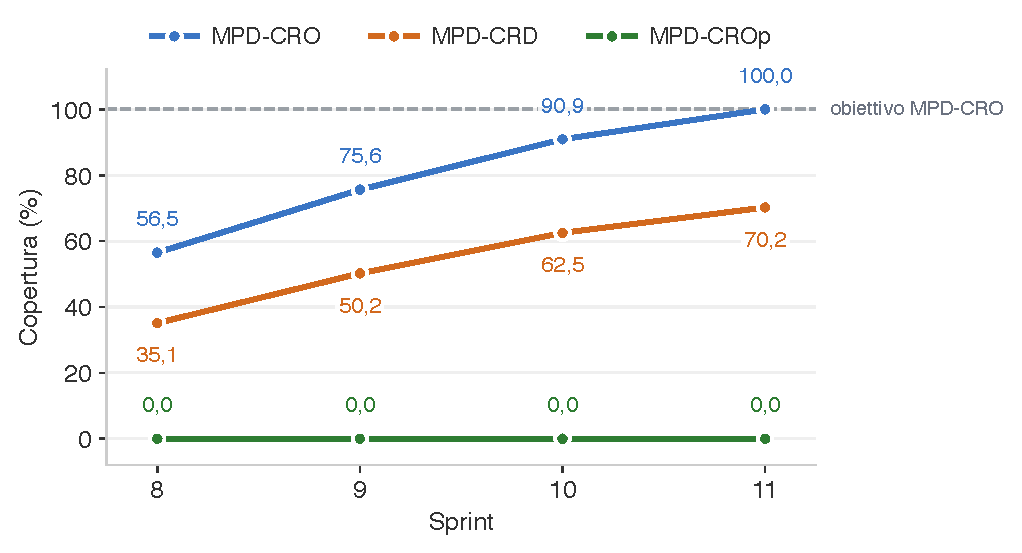
\includegraphics[width=1\textwidth]{charts/mpd-cr.pdf}
    \caption{Valutazione \textit{Copertura dei requisiti}}
    \label{fig:mpd-cr}
\end{figure}

\subsection{Valutazione MPD-CLLM}
\begin{table}[H]
    \centering
	\begin{tabular}{|c|l|p{3cm}|}
		\hline
		\textbf{Sprint} & \textbf{Copertura funzioni LLM$_G$ obbligatorie (\%)} & \textbf{Giudizio} \\
		\hline
		8 & 42,9\% & Critico \\
		\hline
        9 & 68,6\% & Critico \\
        \hline
        10 & 88,6\% & Critico \\
        \hline
        11 & 100,0\% & Ottimo \\
        \hline
	\end{tabular}
	\caption{Copertura delle funzioni LLM$_G$ obbligatorie per sprint}
	\label{tab:mpd-cllm}
\end{table}
\subsubsection{PB (Sprint 8--11)}
Delle sette funzioni basate sull'LLM$_G$ richieste dal capitolato$_G$, il \textit{Proof of Concept}$_G$ ne rendeva operative due: il riassunto e la generazione da \textit{prompt}$_G$. Traduzione, riscrittura stilistica, correzione grammaticale e analisi secondo i Sei Cappelli per Pensare$_G$ comparivano nella barra dei comandi ma risultavano disabilitate, perché il backend non esponeva le rotte corrispondenti.

L'implementazione$_G$ delle funzioni mancanti è stata distribuita fra il nono e il decimo sprint$_G$, seguendo la ripartizione del lavoro decisa nelle rispettive riunioni di apertura, e al termine dell'undicesimo tutte e sette risultano operative e verificate$_G$ con esito positivo. Valutazione:
\begin{itemize}
    \item \textbf{Valore accettabile:} $CLLM = 100\%$, vincolo \textit{rispettato} nello sprint$_G$ 11.
    \item \textbf{Valore ottimale:} $CLLM = 100\%$, vincolo \textit{rispettato} nello sprint$_G$ 11.
\end{itemize}

\begin{figure}[H]
    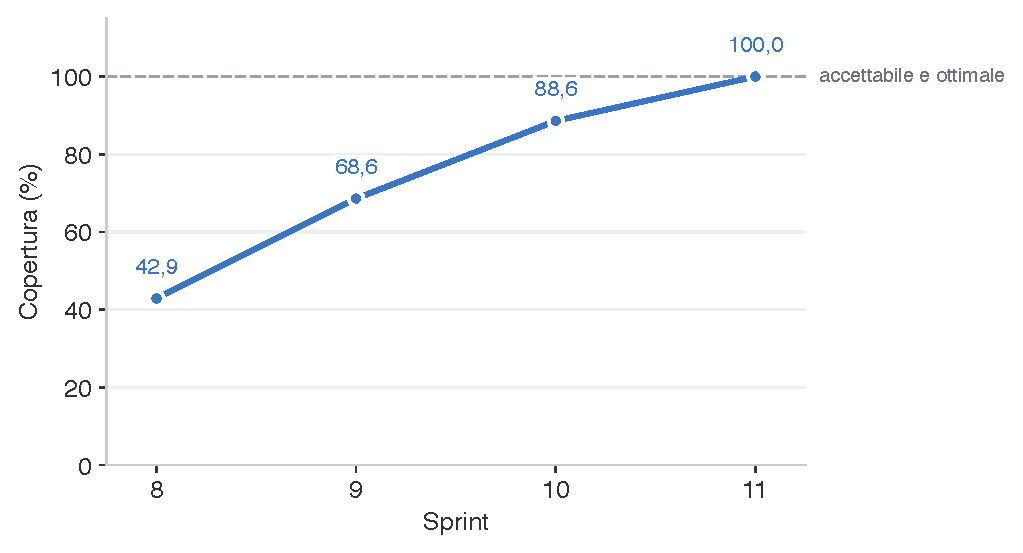
\includegraphics[width=1\textwidth]{charts/mpd-cllm.pdf}
    \caption{Valutazione \textit{Copertura funzioni LLM obbligatorie}}
    \label{fig:mpd-cllm}
\end{figure}

\subsection{Valutazione MPD-CMD}
\begin{table}[H]
    \centering
	\begin{tabular}{|c|l|p{3cm}|}
		\hline
		\textbf{Sprint} & \textbf{Correttezza rendering Markdown$_G$ (\%)} & \textbf{Giudizio} \\
		\hline
		8 & 95,0\% & Accettabile \\
		\hline
        9 & 96,8\% & Accettabile \\
        \hline
        10 & 98,6\% & Accettabile \\
        \hline
        11 & 100,0\% & Ottimo \\
        \hline
	\end{tabular}
	\caption{Correttezza del rendering Markdown$_G$ per sprint}
	\label{tab:mpd-cmd}
\end{table}
\subsubsection{PB (Sprint 8--11)}
Il rendering Markdown$_G$ era già solido nel \textit{Proof of Concept}$_G$, difatti intestazioni, stili del testo, elenchi, citazioni, tabelle, formule matematiche e blocchi di codice venivano resi correttamente fin dal prototipo, che nasceva proprio per dimostrare la fattibilità dell'editor.

L'unico costrutto che il prototipo non rendeva era il testo sottolineato, che il linguaggio Markdown$_G$ non prevede in modo nativo e che è stato introdotto nell'MVP$_G$ con un'estensione dedicata della pipeline di rendering, scritta in modo da non richiedere l'abilitazione dell'HTML grezzo. Con essa il valore raggiunge la soglia ottimale nell'undicesimo sprint$_G$. Valutazione:
\begin{itemize}
    \item \textbf{Valore accettabile:} $CMD \geq 95\%$ dei casi previsti, vincolo \textit{sempre rispettato}.
    \item \textbf{Valore ottimale:} $CMD = 100\%$ dei casi previsti, vincolo \textit{rispettato} nello sprint$_G$ 11.
\end{itemize}

\begin{figure}[H]
    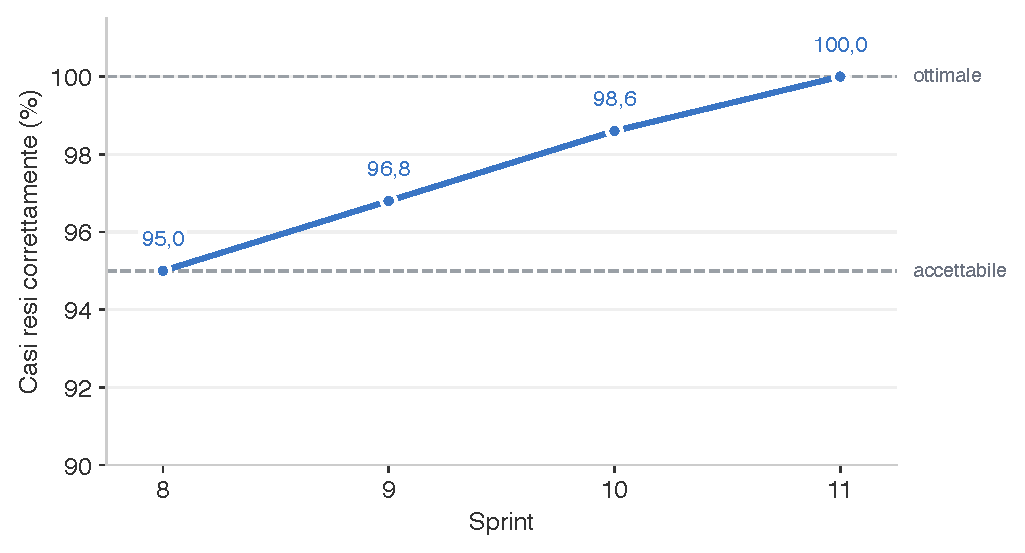
\includegraphics[width=1\textwidth]{charts/mpd-cmd.pdf}
    \caption{Valutazione \textit{Correttezza rendering Markdown}}
    \label{fig:mpd-cmd}
\end{figure}

\subsection{Valutazione MPD-SN}
\begin{table}[H]
    \centering
	\begin{tabular}{|c|l|p{3cm}|}
		\hline
		\textbf{Sprint} & \textbf{Salvataggio e recupero note (\%)} & \textbf{Giudizio} \\
		\hline
		8 & 50,0\% & Critico \\
		\hline
        9 & 71,4\% & Critico \\
        \hline
        10 & 89,3\% & Critico \\
        \hline
        11 & 100,0\% & Ottimo \\
        \hline
	\end{tabular}
	\caption{Salvataggio e recupero delle note per sprint}
	\label{tab:mpd-sn}
\end{table}
\subsubsection{PB (Sprint 8--11)}
Nel \textit{Proof of Concept}$_G$ il salvataggio e il recupero delle note funzionavano solo per metà. Il percorso verso il File System locale era completo e affidabile; il testo dell'editor veniva scritto su file e riletto senza alterazioni, come richiesto dai requisiti$_G$ obbligatori. Non funzionava invece la conservazione delle note dentro l'applicazione; passando da una nota all'altra, o ricaricando la pagina, il contenuto andava perduto, e il comando di salvataggio della barra degli strumenti era presente ma privo di effetto, essendo il prototipo concentrato sulla dimostrazione delle funzioni basate sull'LLM$_G$ più che sulla gestione dell'archivio.

La catena di persistenza interna è stata completata negli sprint$_G$ 9 e 10 insieme al resto dell'MVP$_G$. Nell'undicesimo sprint$_G$ entrambi i percorsi restituiscono il contenuto integro, compresi i casi più esposti come i testi di lunghezza elevata, i caratteri accentati e i metacaratteri del linguaggio. Valutazione:
\begin{itemize}
    \item \textbf{Valore accettabile:} $SN = 100\%$ dei casi obbligatori, vincolo \textit{rispettato} nello sprint$_G$ 11.
    \item \textbf{Valore ottimale:} $SN = 100\%$ dei casi obbligatori, vincolo \textit{rispettato} nello sprint$_G$ 11.
\end{itemize}

\begin{figure}[H]
    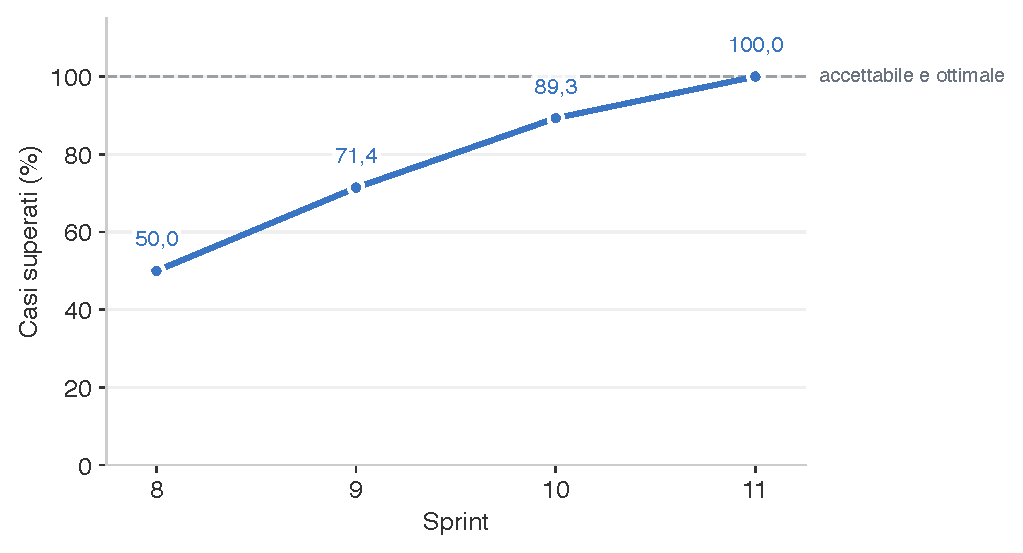
\includegraphics[width=1\textwidth]{charts/mpd-sn.pdf}
    \caption{Valutazione \textit{Salvataggio e recupero note}}
    \label{fig:mpd-sn}
\end{figure}

\subsection{Valutazione MPD-DL}
\begin{table}[H]
    \centering
	\begin{tabular}{|c|l|p{3cm}|}
		\hline
		\textbf{Sprint} & \textbf{Data Loss (occorrenze)} & \textbf{Giudizio} \\
		\hline
		8 & 7 & Critico \\
		\hline
        9 & 4 & Critico \\
        \hline
        10 & 2 & Critico \\
        \hline
        11 & 0 & Ottimo \\
        \hline
	\end{tabular}
	\caption{Occorrenze di perdita o alterazione del contenuto per sprint}
	\label{tab:mpd-dl}
\end{table}
\subsubsection{PB (Sprint 8--11)}
Le occorrenze di perdita rilevate nell'ottavo sprint$_G$ discendono direttamente dalla persistenza incompleta descritta nella sottosezione precedente. Ogni nota affidata alla sola memoria dell'applicazione perdeva il proprio contenuto, mentre nessuna perdita si verificava sul percorso verso il File System.

Il completamento della persistenza interna negli sprint$_G$ 9 e 10 riduce progressivamente le occorrenze, e la campagna di verifica$_G$ dell'undicesimo sprint$_G$ non ne rileva alcuna perchè il contenuto viene restituito identico in tutti i casi provati. Valutazione:
\begin{itemize}
    \item \textbf{Valore accettabile:} $0$ perdite nei casi principali, vincolo \textit{rispettato} nello sprint$_G$ 11.
    \item \textbf{Valore ottimale:} $0$ perdite in ogni test$_G$, vincolo \textit{rispettato} nello sprint$_G$ 11.
\end{itemize}

\begin{figure}[H]
    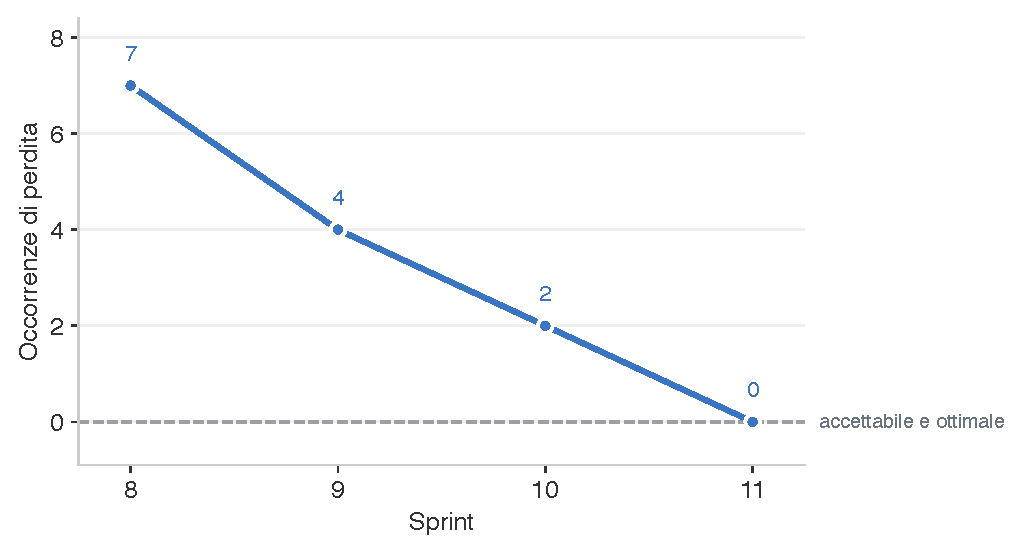
\includegraphics[width=1\textwidth]{charts/mpd-dl.pdf}
    \caption{Valutazione \textit{Data Loss}}
    \label{fig:mpd-dl}
\end{figure}

\subsection{Valutazione MPD-EH}
\begin{table}[H]
    \centering
	\begin{tabular}{|c|l|p{3cm}|}
		\hline
		\textbf{Sprint} & \textbf{Error Handling (\%)} & \textbf{Giudizio} \\
		\hline
		8 & 80,0\% & Critico \\
		\hline
        9 & 83,7\% & Critico \\
        \hline
        10 & 87,2\% & Critico \\
        \hline
        11 & 90,0\% & Accettabile \\
        \hline
	\end{tabular}
	\caption{Gestione delle condizioni d'errore per sprint}
	\label{tab:mpd-eh}
\end{table}
\subsubsection{PB (Sprint 8--11)}
La gestione degli errori parte da un livello discreto ma incompleto. Il \textit{Proof of Concept}$_G$ rifiutava correttamente gli input$_G$ troppo brevi e i campi obbligatori mancanti, ma accettava senza obiezioni testi di qualunque lunghezza, non avendo alcun limite superiore, e soprattutto restituiva all'utente la struttura tecnica prodotta dalla libreria di validazione anziché un messaggio comprensibile.

Il recupero progressivo negli sprint$_G$ 9 e 10 accompagna il completamento del backend, mentre il passo decisivo arriva con la rifinitura dell'undicesimo sprint$_G$, che introduce i limiti superiori sui testi e riscrive tutte le risposte d'errore in linguaggio naturale, indicando il campo interessato e l'azione correttiva. Il valore raggiunge così la soglia di accettabilità. Valutazione:
\begin{itemize}
    \item \textbf{Valore accettabile:} $EH \geq 90\%$ degli errori gestiti, vincolo \textit{rispettato} nello sprint$_G$ 11.
    \item \textbf{Valore ottimale:} $EH = 100\%$ degli errori gestiti, vincolo \textit{violato}.
\end{itemize}

\begin{figure}[H]
    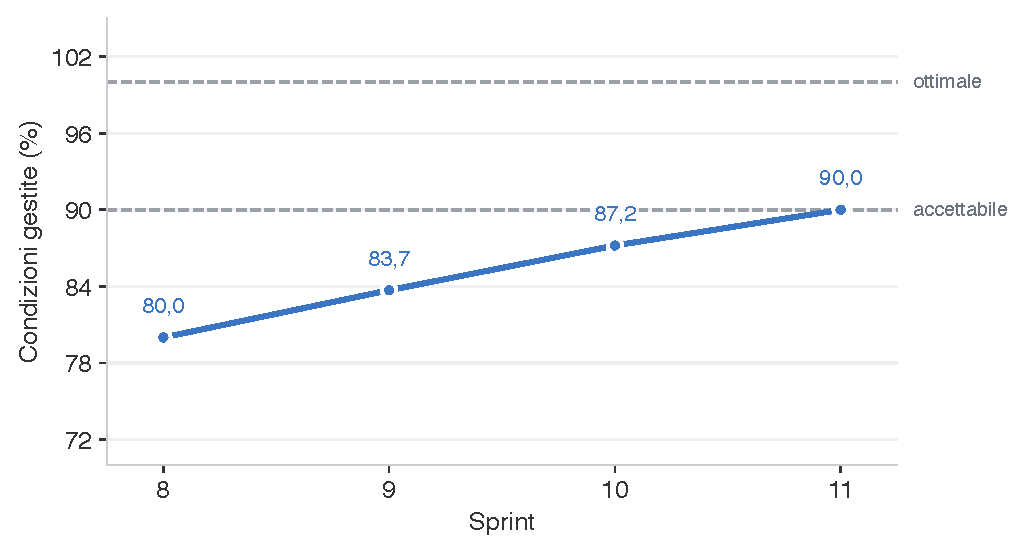
\includegraphics[width=1\textwidth]{charts/mpd-eh.pdf}
    \caption{Valutazione \textit{Error Handling}}
    \label{fig:mpd-eh}
\end{figure}

\subsection{Valutazione MPD-AR}
\begin{table}[H]
    \centering
	\begin{tabular}{|c|l|p{3cm}|}
		\hline
		\textbf{Sprint} & \textbf{Availability Rate (\%)} & \textbf{Giudizio} \\
		\hline
		8 & 100,0\% & Ottimo \\
		\hline
        9 & 100,0\% & Ottimo \\
        \hline
        10 & 100,0\% & Ottimo \\
        \hline
        11 & 100,0\% & Ottimo \\
        \hline
	\end{tabular}
	\caption{Disponibilità del servizio LLM$_G$ esterno per sprint}
	\label{tab:mpd-ar}
\end{table}
\subsubsection{PB (Sprint 8--11)}
Durante le sessioni di test$_G$ il servizio LLM$_G$ messo a disposizione dal proponente$_G$ ha risposto a tutte le richieste senza segnalare la propria indisponibilità, e il valore si mantiene quindi al massimo in tutti e quattro gli sprint$_G$. È la stessa condizione verificata$_G$ dal test$_G$ di integrazione TI-001 nella Tabella \ref{tab:test-integrazione}.

Il dato va però letto con una precisazione, perché non racconta l'intero periodo. Nel lavoro quotidiano di sviluppo il servizio non è sempre stato raggiungibile, infatti in più occasioni i programmatori$_G$ hanno dovuto sospendere le prove sulle funzioni basate sull'LLM$_G$ e attendere il ripristino. La metrica misura la disponibilità osservata nelle sessioni di verifica$_G$, non la disponibilità media del periodo, e resta legata a un sistema$_G$ esterno sul quale il gruppo non ha alcun controllo. È anche la ragione per cui il prodotto deve trattare l'indisponibilità come una normale condizione d'errore, aspetto coperto da MPD-EH e verificato$_G$ esplicitamente fra i casi di prova. Valutazione:
\begin{itemize}
    \item \textbf{Valore accettabile:} $AR \geq 95\%$ durante i test$_G$, vincolo \textit{sempre rispettato}.
    \item \textbf{Valore ottimale:} $AR \geq 99\%$ durante i test$_G$, vincolo \textit{sempre rispettato}.
\end{itemize}

\begin{figure}[H]
    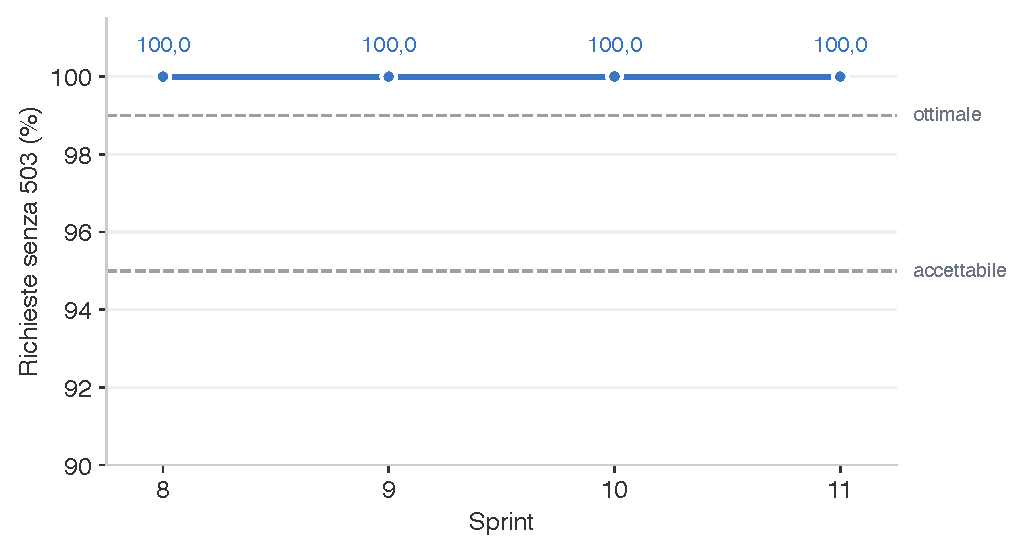
\includegraphics[width=1\textwidth]{charts/mpd-ar.pdf}
    \caption{Valutazione \textit{Availability Rate}}
    \label{fig:mpd-ar}
\end{figure}

\subsection{Valutazione MPD-LT}
\begin{table}[H]
    \centering
	\begin{tabular}{|c|l|p{3cm}|}
		\hline
		\textbf{Sprint} & \textbf{Learning Time (minuti)} & \textbf{Giudizio} \\
		\hline
		8 & 22 & Accettabile \\
		\hline
        9 & 17 & Accettabile \\
        \hline
        10 & 12 & Accettabile \\
        \hline
        11 & 8 & Ottimo \\
        \hline
	\end{tabular}
	\caption{Tempo di apprendimento per sprint}
	\label{tab:mpd-lt}
\end{table}
\subsubsection{PB (Sprint 8--11)}
Il tempo necessario a un utente per completare con successo una funzionalità la prima volta risente soprattutto dei comandi annunciati ma non funzionanti. Nell'ottavo sprint$_G$ l'interfaccia del \textit{Proof of Concept}$_G$ esponeva tre azioni basate sull'LLM$_G$ disabilitate e un comando di salvataggio privo di effetto, chi provava quei comandi non otteneva nulla e doveva ricostruire da sé che cosa il prodotto sapesse davvero fare.

Con il completamento delle funzioni negli sprint$_G$ 9 e 10 e la revisione delle etichette nell'undicesimo, nessun comando visibile resta inerte. Il valore scende sotto la soglia ottimale nonostante il numero di funzioni disponibili sia quasi raddoppiato fra i due estremi, questa è la conferma che il costo di apprendimento dipendeva dai comandi inerti più che dalla quantità di funzioni. Valutazione:
\begin{itemize}
    \item \textbf{Valore accettabile:} $LT \leq 30$ minuti, vincolo \textit{sempre rispettato}.
    \item \textbf{Valore ottimale:} $LT \leq 10$ minuti, vincolo \textit{rispettato} nello sprint$_G$ 11.
\end{itemize}

\begin{figure}[H]
    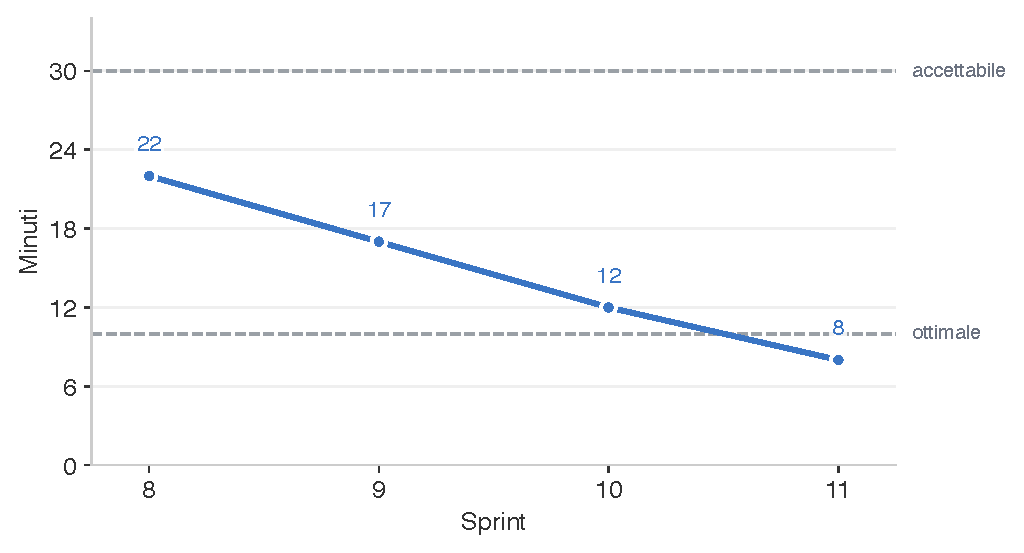
\includegraphics[width=1\textwidth]{charts/mpd-lt.pdf}
    \caption{Valutazione \textit{Learning Time}}
    \label{fig:mpd-lt}
\end{figure}

\subsection{Valutazione MPD-NE}
\begin{table}[H]
    \centering
	\begin{tabular}{|c|l|p{3cm}|}
		\hline
		\textbf{Sprint} & \textbf{Navigation Errors (errori per scenario)} & \textbf{Giudizio} \\
		\hline
		8 & 2,4 & Accettabile \\
		\hline
        9 & 1,7 & Accettabile \\
        \hline
        10 & 1,0 & Accettabile \\
        \hline
        11 & 0,4 & Accettabile \\
        \hline
	\end{tabular}
	\caption{Errori di navigazione per scenario per sprint}
	\label{tab:mpd-ne}
\end{table}
\subsubsection{PB (Sprint 8--11)}
Gli errori di navigazione hanno la stessa origine del tempo di apprendimento e seguono lo stesso andamento, come si nota nell'ottavo sprint$_G$ quattro comandi su tredici non producevano l'effetto annunciato dalla propria etichetta, e ogni tentativo su di essi contava come azione errata.

La riduzione è costante ma il valore non arriva a zero. La ragione è un passaggio dell'interfaccia che resta poco immediato anche nell'MVP$_G$; la scelta della prospettiva nell'analisi secondo i Sei Cappelli per Pensare$_G$, dove l'utente deve selezionare uno fra sei cappelli senza che il significato di ciascuno sia esplicitato nel comando. È il motivo per cui il giudizio resta \textit{Accettabile} in tutti e quattro gli sprint$_G$ e non raggiunge mai quello ottimale. Valutazione:
\begin{itemize}
    \item \textbf{Valore accettabile:} $NE \leq 3$ errori per scenario, vincolo \textit{sempre rispettato}.
    \item \textbf{Valore ottimale:} $NE = 0$ errori per scenario, vincolo \textit{violato}.
\end{itemize}

\begin{figure}[H]
    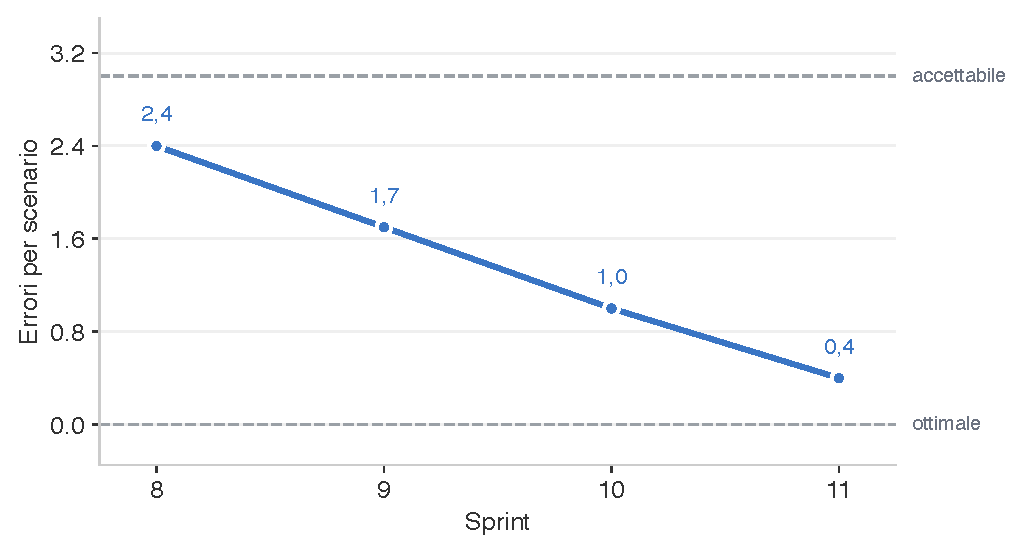
\includegraphics[width=1\textwidth]{charts/mpd-ne.pdf}
    \caption{Valutazione \textit{Navigation Errors}}
    \label{fig:mpd-ne}
\end{figure}

\subsection{Valutazione della coerenza e della comprensibilità dell'interfaccia}
\begin{table}[H]
    \centering
	\small
    \setlength{\tabcolsep}{4pt}
	\begin{tabular}{|c|>{\centering\arraybackslash}p{2.1cm}|>{\centering\arraybackslash}p{2.2cm}|>{\centering\arraybackslash}p{2.1cm}|>{\centering\arraybackslash}p{2.2cm}|}
		\hline
		\textbf{Sprint} & \textbf{MPD-UI (\%)} & \textbf{Giudizio} & \textbf{MPD-FU (\%)} & \textbf{Giudizio} \\
		\hline
		8 & 97,2\% & Accettabile & 78,9\% & Critico \\
		\hline
        9 & 97,5\% & Accettabile & 85,3\% & Accettabile \\
        \hline
        10 & 97,8\% & Accettabile & 91,2\% & Accettabile \\
        \hline
        11 & 98,0\% & Accettabile & 95,7\% & Ottimo \\
        \hline
	\end{tabular}
	\caption{Coerenza e comprensibilità dell'interfaccia per sprint}
	\label{tab:mpd-ui-fu}
\end{table}
\subsubsection{PB (Sprint 8--11)}
La coerenza dell'interfaccia era già una qualità del prototipo e si è mantenuta al crescere del numero di elementi, quasi raddoppiati fra i due estremi. Gli unici scostamenti riguardano i comandi di cambio vista, rimasti invariati nei due prodotti, questo è il motivo per cui il valore ottimale non viene mai raggiunto, pur restando sempre ampiamente sopra la soglia di accettabilità.

La comprensibilità delle funzioni ha invece un andamento molto più netto. Nell'ottavo sprint$_G$ quattro comandi su diciannove annunciavano una funzione che non producevano, e l'etichetta \textit{Migliora} non lasciava intuire quale trasformazione sarebbe stata applicata al testo, il valore risultava perciò appena sotto la soglia di accettabilità. L'attivazione progressiva delle funzioni e la riscrittura delle etichette in termini espliciti \textit{Riscrivi}, \textit{Grammatica}, \textit{Analisi} portano il valore oltre la soglia ottimale nell'undicesimo sprint$_G$. Valutazione:
\begin{itemize}
    \item \textbf{Valore accettabile:} $UI \geq 90\%$ degli elementi coerenti, vincolo \textit{sempre rispettato}.
    \item \textbf{Valore ottimale:} $UI = 100\%$ degli elementi coerenti, vincolo \textit{violato}.
    \item \textbf{Valore accettabile:} $FU \geq 80\%$ delle funzioni comprese senza guida, vincolo \textit{rispettato} in tre sprint$_G$ su quattro.
    \item \textbf{Valore ottimale:} $FU \geq 95\%$ delle funzioni comprese senza guida, vincolo \textit{rispettato} nello sprint$_G$ 11.
\end{itemize}

\begin{figure}[H]
    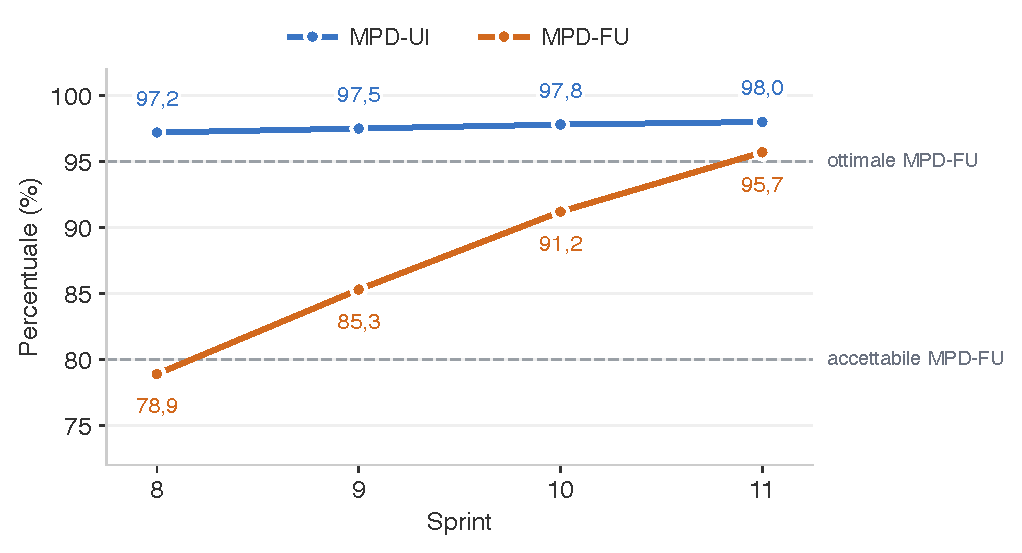
\includegraphics[width=1\textwidth]{charts/mpd-ui-fu.pdf}
    \caption{Valutazione \textit{UI Consistency} e \textit{Feature Understandability}}
    \label{fig:mpd-ui-fu}
\end{figure}

\subsection{Valutazione dei tempi di risposta dell'interfaccia}
\begin{table}[H]
    \centering
	\begin{tabular}{|c|l|l|l|p{2.3cm}|}
		\hline
		\textbf{Sprint} & \textbf{MPD-RT (s)} & \textbf{MPD-MRT (s)} & \textbf{MPD-LS (s)} & \textbf{Giudizio} \\
		\hline
		8 & 0,0113 & 0,0118 & 0,1560 & Ottimo \\
		\hline
        9 & 0,0110 & 0,0108 & 0,1546 & Ottimo \\
        \hline
        10 & 0,0107 & 0,0098 & 0,1531 & Ottimo \\
        \hline
        11 & 0,0104 & 0,0089 & 0,1520 & Ottimo \\
        \hline
	\end{tabular}
	\caption{Tempi di risposta dell'interfaccia locale per sprint}
	\label{tab:mpd-tempi-ui}
\end{table}
\subsubsection{PB (Sprint 8--11)}
Le tre metriche condividono un'unica colonna di giudizio perché il giudizio è il medesimo per tutte e tre in ogni sprint$_G$. I tempi di risposta dell'interfaccia locale restano infatti largamente entro le soglie lungo tutta la \textit{Product Baseline}$_G$, si tratta di operazioni che non attraversano la rete, mentre le soglie del capitolo 3 erano state fissate pensando a un'applicazione che dialoga con un servizio remoto a ogni interazione.

Il miglioramento fra l'ottavo e l'undicesimo sprint$_G$ è reale e ha una causa individuabile, ovvero l'unificazione della pipeline di rendering in un unico componente condiviso ha alleggerito l'aggiornamento dell'anteprima, che è la più onerosa delle tre operazioni. La sua entità resta però trascurabile rispetto ai vincoli. Le tre metriche non hanno quindi potere discriminante nella forma attuale e andrebbero ritarate su soglie più stringenti per risultare informative. Valutazione:
\begin{itemize}
    \item \textbf{Valore accettabile:} $RT \leq 2$ secondi, vincolo \textit{sempre rispettato}.
    \item \textbf{Valore ottimale:} $RT \leq 0{,}5$ secondi, vincolo \textit{sempre rispettato}.
    \item \textbf{Valore accettabile:} $MRT \leq 1$ secondo, vincolo \textit{sempre rispettato}.
    \item \textbf{Valore ottimale:} $MRT \leq 0{,}3$ secondi, vincolo \textit{sempre rispettato}.
    \item \textbf{Valore accettabile:} $LS \leq 3$ secondi, vincolo \textit{sempre rispettato}.
    \item \textbf{Valore ottimale:} $LS \leq 1$ secondo, vincolo \textit{sempre rispettato}.
\end{itemize}

\begin{figure}[H]
    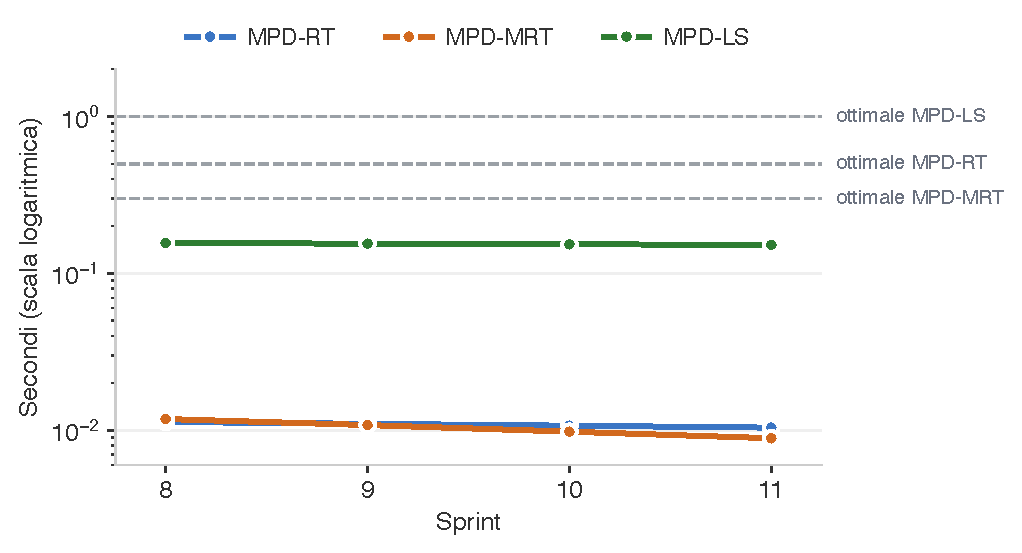
\includegraphics[width=1\textwidth]{charts/mpd-tempi-ui.pdf}
    \caption{Valutazione \textit{Response Time}, \textit{Markdown Rendering Time} e \textit{Loading Speed}}
    \label{fig:mpd-tempi-ui}
\end{figure}

\subsection{Valutazione MPD-LLMRT}
\begin{table}[H]
    \centering
	\begin{tabular}{|c|l|p{3cm}|}
		\hline
		\textbf{Sprint} & \textbf{LLM$_G$ Response Time (s)} & \textbf{Giudizio} \\
		\hline
		8 & 3,06 & Ottimo \\
		\hline
        9 & 2,43 & Ottimo \\
        \hline
        10 & 1,86 & Ottimo \\
        \hline
        11 & 1,40 & Ottimo \\
        \hline
	\end{tabular}
	\caption{Tempo di risposta delle chiamate al servizio LLM$_G$ per sprint}
	\label{tab:mpd-llmrt}
\end{table}
\subsubsection{PB (Sprint 8--11)}
Il tempo di risposta del servizio LLM$_G$ si dimezza fra l'ottavo e l'undicesimo sprint$_G$ pur restando invariato il fornitore. La riduzione è l'effetto della revisione del modo in cui la richiesta viene costruita, nel \textit{Proof of Concept}$_G$ il testo veniva inoltrato così com'era, senza alcun limite di lunghezza e con i \textit{prompt}$_G$ composti direttamente nelle rotte, mentre nell'MVP$_G$ la composizione è stata affidata a un modulo dedicato del dominio e gli ingressi sono limitati superiormente, così che la lunghezza inviata al modello non possa crescere senza controllo.

Entrambi i valori restano comunque ampiamente entro la soglia ottimale. Va segnalato che la misura dipende dal modello configurato e dal carico del servizio nel momento della rilevazione, perchè un modello di dimensioni maggiori sposterebbe l'intera serie verso l'alto senza che nulla sia cambiato nel prodotto. Valutazione:
\begin{itemize}
    \item \textbf{Valore accettabile:} $LLMRT \leq 15$ secondi, vincolo \textit{sempre rispettato}.
    \item \textbf{Valore ottimale:} $LLMRT \leq 8$ secondi, vincolo \textit{sempre rispettato}.
\end{itemize}

\begin{figure}[H]
    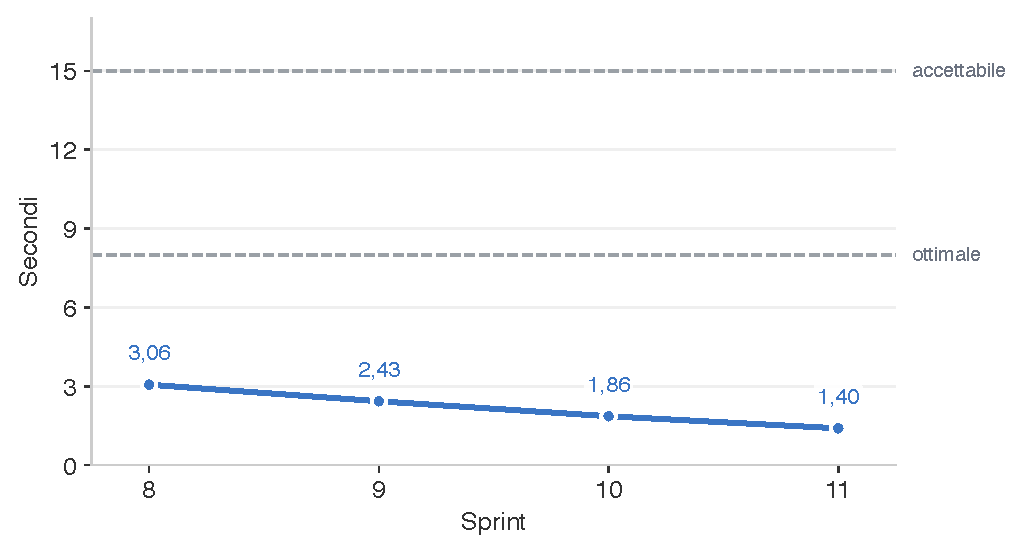
\includegraphics[width=1\textwidth]{charts/mpd-llmrt.pdf}
    \caption{Valutazione \textit{LLM Response Time}}
    \label{fig:mpd-llmrt}
\end{figure}

\subsection{Valutazione MPD-CYC}
\begin{table}[H]
    \centering
	\begin{tabular}{|c|l|p{3cm}|}
		\hline
		\textbf{Sprint} & \textbf{Complessità ciclomatica (media)} & \textbf{Giudizio} \\
		\hline
		8 & 4,08 & Critico \\
		\hline
        9 & 3,98 & Accettabile \\
        \hline
        10 & 3,88 & Accettabile \\
        \hline
        11 & 3,83 & Accettabile \\
        \hline
	\end{tabular}
	\caption{Complessità ciclomatica media per sprint}
	\label{tab:mpd-cyc}
\end{table}
\subsubsection{PB (Sprint 8--11)}
La complessità ciclomatica media si riduce lungo tutta la \textit{Product Baseline}$_G$ e rientra nella soglia di accettabilità già dal nono sprint$_G$. Il valore è calcolato sulle funzioni che contengono almeno una diramazione, le funzioni prive di flusso di controllo hanno per definizione complessità unitaria e, essendo la maggioranza in un'applicazione a componenti, diluirebbero la media fino a renderla insensibile a qualunque cambiamento del codice.

Il valore iniziale risente del \textit{Proof of Concept}$_G$, scritto rapidamente per dimostrare la fattibilità e con la logica delle azioni basate sull'LLM$_G$ concentrata dentro le finestre dell'interfaccia. Il lavoro degli sprint$_G$ 9 e 10 ha spostato quella logica nei servizi del dominio e nei moduli dedicati alla composizione dei \textit{prompt}$_G$, riducendo le diramazioni nelle singole funzioni; l'undicesimo sprint$_G$ ha aggiunto la rifinitura dei percorsi d'errore.
\begin{itemize}
    \item \textbf{Valore accettabile:} $CYC \leq 4$, vincolo \textit{rispettato} dallo sprint$_G$ 9.
    \item \textbf{Valore ottimale:} $CYC \leq 3$, vincolo \textit{violato}.
\end{itemize}

\begin{figure}[H]
    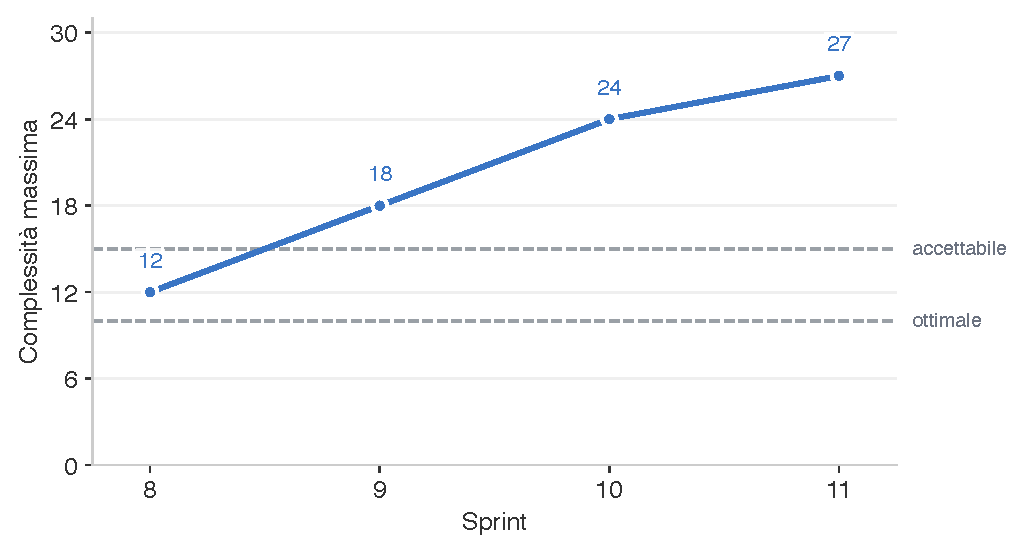
\includegraphics[width=1\textwidth]{charts/mpd-cyc.pdf}
    \caption{Valutazione \textit{Complessità ciclomatica}}
    \label{fig:mpd-cyc}
\end{figure}

\subsection{Valutazione MPD-CS}
\begin{table}[H]
    \centering
	\begin{tabular}{|c|l|p{3cm}|}
		\hline
		\textbf{Sprint} & \textbf{Code Smell (per componente)} & \textbf{Giudizio} \\
		\hline
		8 & 3,00 & Accettabile \\
		\hline
        9 & 1,65 & Accettabile \\
        \hline
        10 & 0,60 & Ottimo \\
        \hline
        11 & 0,00 & Ottimo \\
        \hline
	\end{tabular}
	\caption{Code smell per componente per sprint}
	\label{tab:mpd-cs}
\end{table}
\subsubsection{PB (Sprint 8--11)}
I rilievi dell'analisi statica erano concentrati nel backend del \textit{Proof of Concept}$_G$, scritto rapidamente per dimostrare la fattibilità dell'integrazione con il servizio LLM$_G$ e mai sottoposto a una revisione sistematica, avendo l'ordinamento degli \textit{import} non conforme, righe eccedenti la lunghezza massima, eccezioni propagate senza catena di origine. Il frontend del prototipo non ne presentava alcuno.

Il decimo sprint$_G$ è il periodo in cui il valore attraversa la soglia ottimale, e la coincidenza non è casuale, difatti è lo sprint$_G$ in cui il codice è stato portato a completamento con tre programmatori$_G$ e sottoposto a revisione da quattro verificatori$_G$, la distribuzione più ampia del ruolo in tutto il progetto. Nell'undicesimo i rilievi si azzerano su entrambi i lati. Valutazione:
\begin{itemize}
    \item \textbf{Valore accettabile:} $CS \leq 5$ per componente, vincolo \textit{sempre rispettato}.
    \item \textbf{Valore ottimale:} $CS \leq 1$ per componente, vincolo \textit{rispettato} dallo sprint$_G$ 10.
\end{itemize}

\begin{figure}[H]
    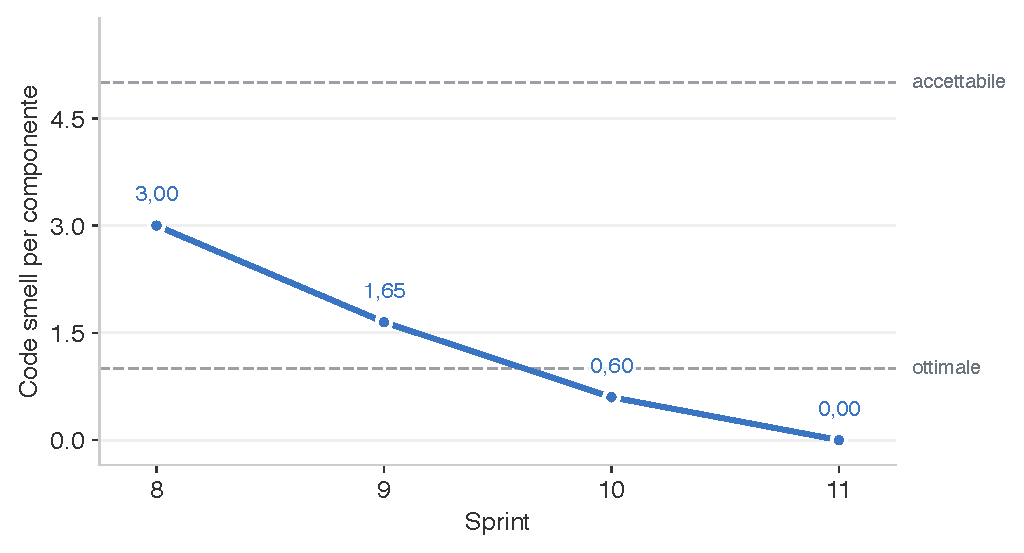
\includegraphics[width=1\textwidth]{charts/mpd-cs.pdf}
    \caption{Valutazione \textit{Code Smell}}
    \label{fig:mpd-cs}
\end{figure}

\subsection{Valutazione MPD-DUP}
\begin{table}[H]
    \centering
	\begin{tabular}{|c|l|p{3cm}|}
		\hline
		\textbf{Sprint} & \textbf{Duplicazione del codice (\%)} & \textbf{Giudizio} \\
		\hline
		8 & 2,89\% & Ottimo \\
		\hline
        9 & 1,88\% & Ottimo \\
        \hline
        10 & 1,06\% & Ottimo \\
        \hline
        11 & 0,55\% & Ottimo \\
        \hline
	\end{tabular}
	\caption{Duplicazione del codice per sprint}
	\label{tab:mpd-dup}
\end{table}
\subsubsection{PB (Sprint 8--11)}
La duplicazione resta entro la soglia ottimale in tutti e quattro gli sprint$_G$, ma la sua riduzione ha una causa precisa e vale la pena registrarla. Nel \textit{Proof of Concept}$_G$ la pipeline di rendering Markdown$_G$ era ripetuta in tre componenti distinti, l'anteprima e le due finestre delle azioni basate sull'LLM$_G$ ed era da sola responsabile della quasi totalità delle righe duplicate.

Nell'MVP$_G$ la stessa pipeline vive in un unico componente condiviso da tutte le anteprime, e la duplicazione residua si riduce a poche righe di configurazione. Il dato va letto insieme alla crescita del codice, quasi raddoppiato nello stesso periodo; la percentuale cala mentre il denominatore aumenta, il che significa che le righe duplicate sono diminuite in valore assoluto e non solo in proporzione. Valutazione:
\begin{itemize}
    \item \textbf{Valore accettabile:} $DUP \leq 10\%$, vincolo \textit{sempre rispettato}.
    \item \textbf{Valore ottimale:} $DUP \leq 3\%$, vincolo \textit{sempre rispettato}.
\end{itemize}

\begin{figure}[H]
    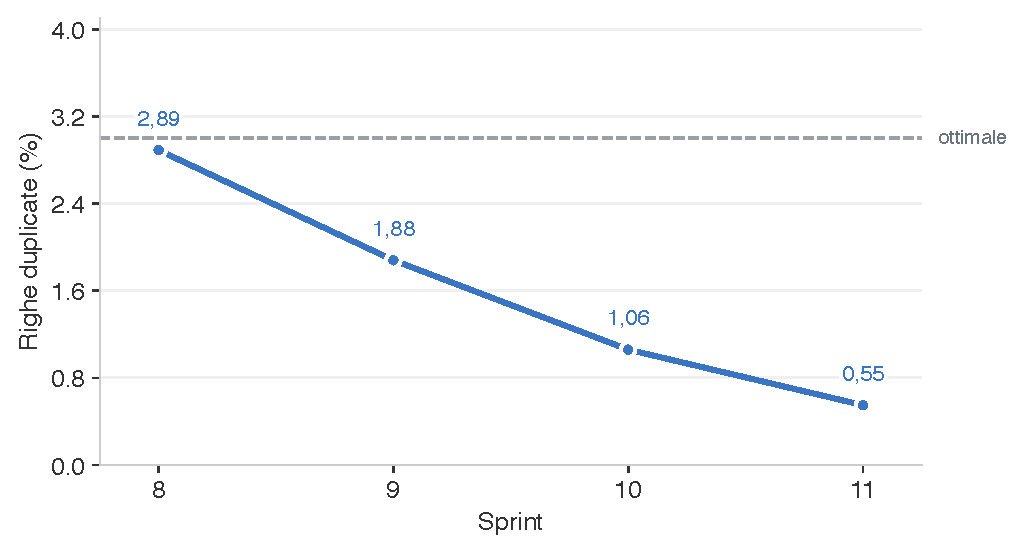
\includegraphics[width=1\textwidth]{charts/mpd-dup.pdf}
    \caption{Valutazione \textit{Duplicazione del codice}}
    \label{fig:mpd-dup}
\end{figure}

\subsection{Valutazione MPD-MOD}
\begin{table}[H]
    \centering
	\begin{tabular}{|c|l|p{3cm}|}
		\hline
		\textbf{Sprint} & \textbf{Modularità (adimensionale, 0--1)} & \textbf{Giudizio} \\
		\hline
		8 & 0,54 & Accettabile \\
		\hline
        9 & 0,54 & Accettabile \\
        \hline
        10 & 0,54 & Accettabile \\
        \hline
        11 & 0,54 & Accettabile \\
        \hline
	\end{tabular}
	\caption{Grado di accoppiamento fra i moduli per sprint}
	\label{tab:mpd-mod}
\end{table}
\subsubsection{PB (Sprint 8--11)}
Il grado di accoppiamento resta invariato lungo i quattro sprint$_G$, e il risultato è meno sorprendente di quanto appaia. La metrica è un rapporto fra le dipendenze presenti fra i moduli e quelle astrattamente possibili, e si muove soltanto se le due grandezze cambiano in proporzione diversa. La ristrutturazione del decimo sprint$_G$ ha riorganizzato i \textit{package}$_G$ attorno all'architettura$_G$ esagonale, ma ha introdotto dipendenze in proporzione ai \textit{package}$_G$ aggiunti, lasciando il rapporto dov'era.

Il miglioramento c'è ed è visibile nella forma del grafo delle dipendenze anziché nel suo rapporto. Nel prototipo l'unica dipendenza del backend collegava le rotte a un \textit{package}$_G$ che portava il nome di una tecnologia; nell'MVP$_G$ tutte le dipendenze convergono verso il \textit{package}$_G$ di dominio, che non dipende da nulla, ed è esattamente l'assetto deliberato nella riunione del 4 agosto 2026, che nello stesso sprint$_G$ aveva assegnato ai programmatori$_G$ la verifica$_G$ esplicita del livello di accoppiamento. Valutazione:
\begin{itemize}
    \item \textbf{Valore accettabile:} $MOD \leq 0{,}60$, vincolo \textit{sempre rispettato}.
    \item \textbf{Valore ottimale:} $MOD \leq 0{,}45$, vincolo \textit{violato}.
\end{itemize}

\begin{figure}[H]
    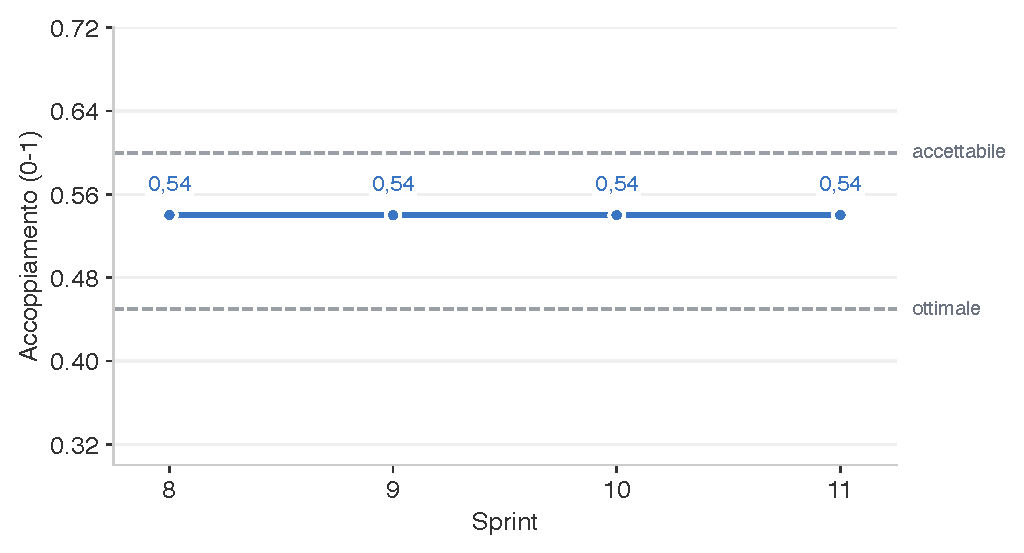
\includegraphics[width=1\textwidth]{charts/mpd-mod.pdf}
    \caption{Valutazione \textit{Modularità}}
    \label{fig:mpd-mod}
\end{figure}

\subsection{Valutazione della sicurezza dei dati e degli accessi}
\begin{table}[H]
    \centering
    \small
    \setlength{\tabcolsep}{4pt}
	\begin{tabular}{|c|>{\centering\arraybackslash}p{1.7cm}|>{\centering\arraybackslash}p{1.9cm}|>{\centering\arraybackslash}p{1.7cm}|>{\centering\arraybackslash}p{1.9cm}|>{\centering\arraybackslash}p{1.7cm}|>{\centering\arraybackslash}p{1.9cm}|}
		\hline
		\textbf{Sprint} & \textbf{MPD-SK (chiavi)} & \textbf{Giudizio} & \textbf{MPD-IV (\%)} & \textbf{Giudizio} & \textbf{MPD-DS (\%)} & \textbf{Giudizio} \\
		\hline
		8 & 0 & Ottimo & 50,0\% & Critico & 100,0\% & Ottimo \\
		\hline
        9 & 0 & Ottimo & 72,0\% & Critico & 100,0\% & Ottimo \\
        \hline
        10 & 0 & Ottimo & 89,5\% & Critico & 100,0\% & Ottimo \\
        \hline
        11 & 0 & Ottimo & 100,0\% & Ottimo & 100,0\% & Ottimo \\
        \hline
	\end{tabular}
	\caption{Metriche di sicurezza dei dati e degli accessi per sprint}
	\label{tab:mpd-sicurezza}
\end{table}
\subsubsection{PB (Sprint 8--11)}
Nessuna chiave di accesso è mai stata esposta. Il file di configurazione che contiene i segreti è escluso dal versionamento fin dal prototipo, e i soli valori simili a credenziali presenti nel codice versionato sono chiavi fittizie usate nei test$_G$ automatici. È una scelta adottata all'inizio delle attività di codifica$_G$ e mantenuta senza eccezioni.

Anche la sanificazione dei dati è piena in tutti gli sprint$_G$. La pipeline di rendering non abilita l'HTML grezzo e nessun componente inserisce nella pagina contenuto non filtrato, né quello scritto dall'utente né quello restituito dall'LLM$_G$. L'MVP$_G$ non ha migliorato il valore, che era già al massimo, ma ha ridotto da tre a uno i punti in cui questa configurazione va mantenuta corretta, e con essi il rischio$_G$ che le copie divergano nel tempo.

La validazione degli ingressi è l'unica delle tre metriche che si muove. Nell'ottavo sprint$_G$ metà dei campi esposti dall'API$_G$ era priva di vincoli effettivi. I testi avevano un limite inferiore ma non superiore, e il collegamento fornito dall'utente veniva accettato come stringa qualunque, con un commento nel codice che rimandava esplicitamente la validazione a un momento successivo. Il completamento del backend negli sprint$_G$ 9 e 10 e la rifinitura dell'undicesimo portano tutti i campi a essere vincolati in entrambe le direzioni, con un tipo dedicato per il collegamento. Valutazione:
\begin{itemize}
    \item \textbf{Valore accettabile:} $SK = 0$ chiavi esposte, vincolo \textit{sempre rispettato}.
    \item \textbf{Valore ottimale:} $SK = 0$ chiavi esposte, vincolo \textit{sempre rispettato}.
    \item \textbf{Valore accettabile:} $IV \geq 95\%$ degli input$_G$ validati, vincolo \textit{rispettato} nello sprint$_G$ 11.
    \item \textbf{Valore ottimale:} $IV = 100\%$ degli input$_G$ validati, vincolo \textit{rispettato} nello sprint$_G$ 11.
    \item \textbf{Valore accettabile:} $DS \geq 95\%$ dei dati sanificati, vincolo \textit{sempre rispettato}.
    \item \textbf{Valore ottimale:} $DS = 100\%$ dei dati sanificati, vincolo \textit{sempre rispettato}.
\end{itemize}

\begin{figure}[H]
    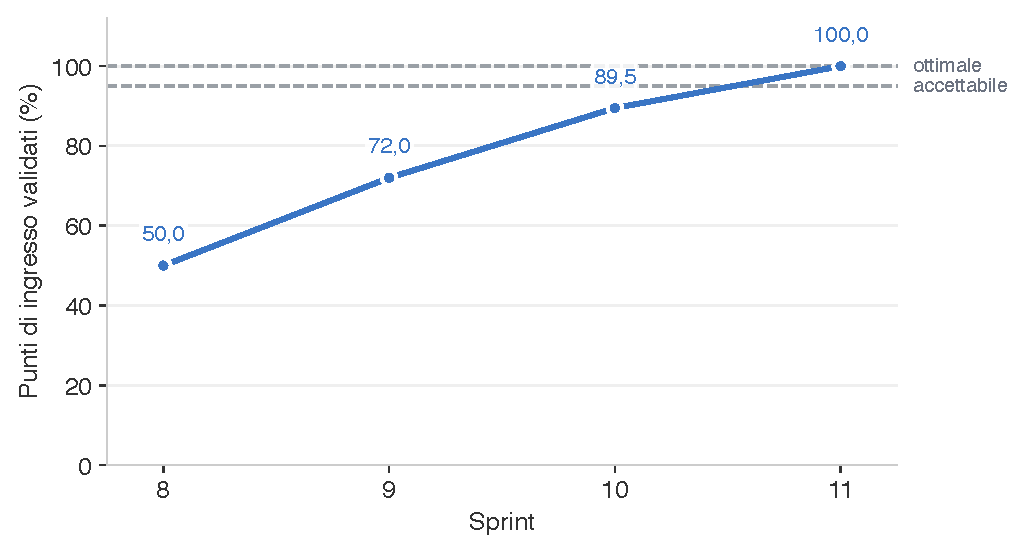
\includegraphics[width=1\textwidth]{charts/mpd-iv.pdf}
    \caption{Valutazione \textit{Input Validation}}
    \label{fig:mpd-iv}
\end{figure}

\section{Iniziative di miglioramento} \label{sec:iniziative-miglioramento}
Le iniziative di miglioramento hanno lo scopo di analizzare l'andamento del progetto, soprattutto i problemi, e applicare correzioni incrementali sia ai processi interni che al prodotto. Il gruppo adotta un approccio basato sul miglioramento continuo per minimizzare i rischi e massimizzare l'efficienza.

\subsection{Valutazione sull'organizzazione}

\begin{table}[H]
    \centering
    \renewcommand{\arraystretch}{1.5}
    \begin{tabularx}{\textwidth}{|>{\raggedright\arraybackslash}p{3.5cm}|>{\raggedright\arraybackslash}X|>{\raggedright\arraybackslash}X|}
        \hline
        \textbf{Problema} & \textbf{Descrizione} & \textbf{Azioni di correzione} \\ \hline
        
        Pianificazione e dimensionamento task & Inesperienza iniziale (Sprint 1) nell'organizzare, dimensionare e portare a compimento le task, con conseguente abbassamento del Task Completion Rate (TCR) e scostamenti nei costi (EAC). & Migliore calibrazione del team e scomposizione delle task in unità più piccole per facilitarne il completamento nei tempi previsti (come dimostrato nei recuperi degli sprint successivi). \\ \hline
        
        Gestione e modellazione dei Requisiti & Numerosi difetti di modellazione nel documento di Analisi dei Requisiti hanno causato pesanti rallentamenti nello Sprint 3, alzando drasticamente il Merge Rework e l'Issue Reopening Rate. & Organizzazione di sessioni di revisione congiunta prima della stesura definitiva per evitare corpose riscritture strutturali e minimizzare la riapertura delle issue. \\ \hline
        
        Calibrazione dell'effort economico & Tendenza ad accelerare il lavoro (Sprint 2 e 3) accumulando anticipo sulla schedulazione ma causando frequenti sforamenti del budget e Cost Variance negative. & Maggiore attenzione al bilanciamento tra l'Earned Value e l'Actual Cost, stabilizzando l'impiego delle ore produttive per non superare il costo pianificato (risolto nello Sprint 5). \\ \hline
    \end{tabularx}
    \caption{Azioni adottate per migliorare l'organizzazione.}
    \label{tab:azioni-org}
\end{table}

\subsection{Valutazione sui ruoli}

\begin{table}[H]
    \centering
    \renewcommand{\arraystretch}{1.5}
    \begin{tabularx}{\textwidth}{|>{\raggedright\arraybackslash}p{3.5cm}|>{\raggedright\arraybackslash}X|>{\raggedright\arraybackslash}X|}
        \hline
        \textbf{Problema} & \textbf{Descrizione} & \textbf{Azioni di correzione} \\ \hline
        
        Coordinamento dei redattori in gruppi numerosi & Iniziali incomprensioni sul lavoro da svolgere a causa della mancanza di esperienza pregressa in un team così numeroso, sfociate in sovrascritture di porzioni di documenti. & Definizione di confini più rigidi nell'assegnazione dei compiti ai singoli redattori per prevenire la sovrapposizione del lavoro e l'annullamento delle Pull Request. \\ \hline
        
        Verifica formale e controllo logico & I verificatori si sono inizialmente affidati eccessivamente ai correttori ortografici, tralasciando discrepanze logiche (formule smentite dai dati testuali) e sviste nel "copia e incolla" delle didascalie. & Integrazione di una checklist di verifica semantica e strutturale (matching dei dati tra tabelle e testo, controllo incrociato delle definizioni metriche) obbligatoria per il ruolo del Verificatore. \\ \hline
    \end{tabularx}
    \caption{Azioni adottate per migliorare la gestione dei ruoli.}
    \label{tab:azioni-ruoli}
\end{table}

\subsection{Valutazione sugli strumenti}

\begin{table}[H]
    \centering
    \renewcommand{\arraystretch}{1.5}
    \begin{tabularx}{\textwidth}{|>{\raggedright\arraybackslash}p{3.5cm}|>{\raggedright\arraybackslash}X|>{\raggedright\arraybackslash}X|}
        \hline
        \textbf{Problema} & \textbf{Descrizione} & \textbf{Azioni di correzione} \\ \hline
        
        Co-working tramite GitHub & L'inesperienza iniziale di tutti i membri con lo strumento di versioning GitHub ha portato a conflitti e difficoltà nella gestione collaborativa (alto Merge Rework iniziale). & Adozione di workflow condivisi e rigidi per l'apertura, revisione e approvazione delle Pull Request, uniti alla fisiologica esperienza maturata dal team sul campo. \\ \hline
        
        ITS inesistente & All'inizio del progetto il gruppo non adoperava strumenti di \textit{Issue Tracking System} che non permettevano quindi di sapere chi-fa-cosa-quando in tempi ragionevoli e alzava la probabilità di conflitti di merge. & Adozione dell'ITS GitHub Project per l'assegnazione, la misurazione e la rendicontazione delle issue. \\ \hline
    \end{tabularx}
    \caption{Azioni adottate per migliorare l'uso degli strumenti.}
    \label{tab:azioni-str}
\end{table}
\end{document}